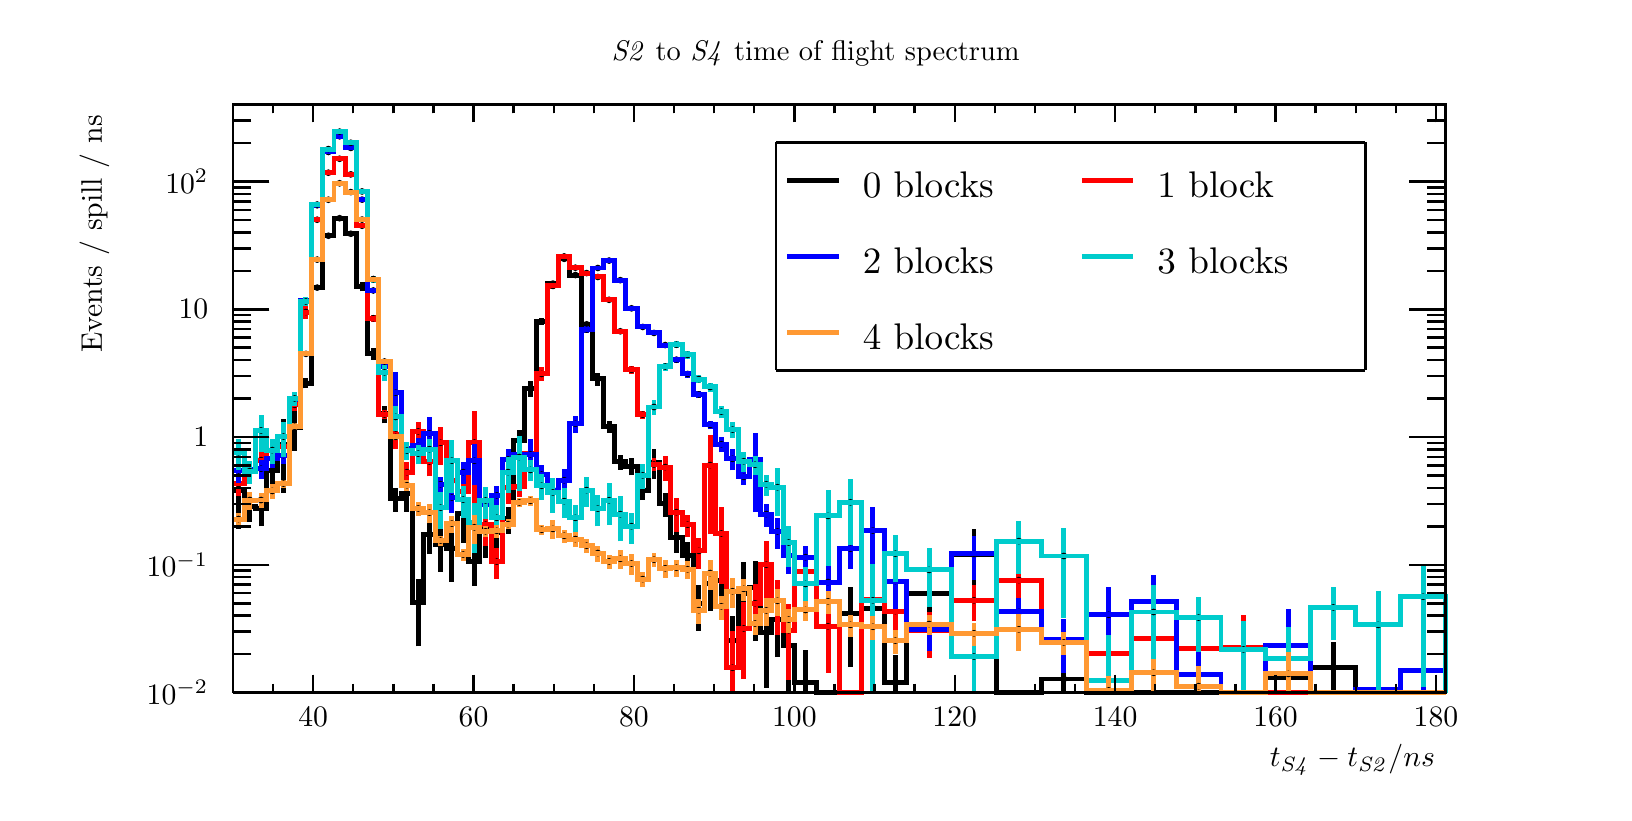
\begin{tikzpicture}
\pgfdeclareplotmark{cross} {
\pgfpathmoveto{\pgfpoint{-0.3\pgfplotmarksize}{\pgfplotmarksize}}
\pgfpathlineto{\pgfpoint{+0.3\pgfplotmarksize}{\pgfplotmarksize}}
\pgfpathlineto{\pgfpoint{+0.3\pgfplotmarksize}{0.3\pgfplotmarksize}}
\pgfpathlineto{\pgfpoint{+1\pgfplotmarksize}{0.3\pgfplotmarksize}}
\pgfpathlineto{\pgfpoint{+1\pgfplotmarksize}{-0.3\pgfplotmarksize}}
\pgfpathlineto{\pgfpoint{+0.3\pgfplotmarksize}{-0.3\pgfplotmarksize}}
\pgfpathlineto{\pgfpoint{+0.3\pgfplotmarksize}{-1.\pgfplotmarksize}}
\pgfpathlineto{\pgfpoint{-0.3\pgfplotmarksize}{-1.\pgfplotmarksize}}
\pgfpathlineto{\pgfpoint{-0.3\pgfplotmarksize}{-0.3\pgfplotmarksize}}
\pgfpathlineto{\pgfpoint{-1.\pgfplotmarksize}{-0.3\pgfplotmarksize}}
\pgfpathlineto{\pgfpoint{-1.\pgfplotmarksize}{0.3\pgfplotmarksize}}
\pgfpathlineto{\pgfpoint{-0.3\pgfplotmarksize}{0.3\pgfplotmarksize}}
\pgfpathclose
\pgfusepathqstroke
}
\pgfdeclareplotmark{cross*} {
\pgfpathmoveto{\pgfpoint{-0.3\pgfplotmarksize}{\pgfplotmarksize}}
\pgfpathlineto{\pgfpoint{+0.3\pgfplotmarksize}{\pgfplotmarksize}}
\pgfpathlineto{\pgfpoint{+0.3\pgfplotmarksize}{0.3\pgfplotmarksize}}
\pgfpathlineto{\pgfpoint{+1\pgfplotmarksize}{0.3\pgfplotmarksize}}
\pgfpathlineto{\pgfpoint{+1\pgfplotmarksize}{-0.3\pgfplotmarksize}}
\pgfpathlineto{\pgfpoint{+0.3\pgfplotmarksize}{-0.3\pgfplotmarksize}}
\pgfpathlineto{\pgfpoint{+0.3\pgfplotmarksize}{-1.\pgfplotmarksize}}
\pgfpathlineto{\pgfpoint{-0.3\pgfplotmarksize}{-1.\pgfplotmarksize}}
\pgfpathlineto{\pgfpoint{-0.3\pgfplotmarksize}{-0.3\pgfplotmarksize}}
\pgfpathlineto{\pgfpoint{-1.\pgfplotmarksize}{-0.3\pgfplotmarksize}}
\pgfpathlineto{\pgfpoint{-1.\pgfplotmarksize}{0.3\pgfplotmarksize}}
\pgfpathlineto{\pgfpoint{-0.3\pgfplotmarksize}{0.3\pgfplotmarksize}}
\pgfpathclose
\pgfusepathqfillstroke
}
\pgfdeclareplotmark{newstar} {
\pgfpathmoveto{\pgfqpoint{0pt}{\pgfplotmarksize}}
\pgfpathlineto{\pgfqpointpolar{44}{0.5\pgfplotmarksize}}
\pgfpathlineto{\pgfqpointpolar{18}{\pgfplotmarksize}}
\pgfpathlineto{\pgfqpointpolar{-20}{0.5\pgfplotmarksize}}
\pgfpathlineto{\pgfqpointpolar{-54}{\pgfplotmarksize}}
\pgfpathlineto{\pgfqpointpolar{-90}{0.5\pgfplotmarksize}}
\pgfpathlineto{\pgfqpointpolar{234}{\pgfplotmarksize}}
\pgfpathlineto{\pgfqpointpolar{198}{0.5\pgfplotmarksize}}
\pgfpathlineto{\pgfqpointpolar{162}{\pgfplotmarksize}}
\pgfpathlineto{\pgfqpointpolar{134}{0.5\pgfplotmarksize}}
\pgfpathclose
\pgfusepathqstroke
}
\pgfdeclareplotmark{newstar*} {
\pgfpathmoveto{\pgfqpoint{0pt}{\pgfplotmarksize}}
\pgfpathlineto{\pgfqpointpolar{44}{0.5\pgfplotmarksize}}
\pgfpathlineto{\pgfqpointpolar{18}{\pgfplotmarksize}}
\pgfpathlineto{\pgfqpointpolar{-20}{0.5\pgfplotmarksize}}
\pgfpathlineto{\pgfqpointpolar{-54}{\pgfplotmarksize}}
\pgfpathlineto{\pgfqpointpolar{-90}{0.5\pgfplotmarksize}}
\pgfpathlineto{\pgfqpointpolar{234}{\pgfplotmarksize}}
\pgfpathlineto{\pgfqpointpolar{198}{0.5\pgfplotmarksize}}
\pgfpathlineto{\pgfqpointpolar{162}{\pgfplotmarksize}}
\pgfpathlineto{\pgfqpointpolar{134}{0.5\pgfplotmarksize}}
\pgfpathclose
\pgfusepathqfillstroke
}
\definecolor{c}{rgb}{1,1,1};
\draw [color=c, fill=c] (0,0) rectangle (20,9.69819);
\draw [color=c, fill=c] (2.6,1.26076) rectangle (18,8.72837);
\definecolor{c}{rgb}{0,0,0};
\draw [c,line width=0.9] (2.6,1.26076) -- (2.6,8.72837) -- (18,8.72837) -- (18,1.26076) -- (2.6,1.26076);
\definecolor{c}{rgb}{1,1,1};
\draw [color=c, fill=c] (2.6,1.26076) rectangle (18,8.72837);
\definecolor{c}{rgb}{0,0,0};
\draw [c,line width=0.9] (2.6,1.26076) -- (2.6,8.72837) -- (18,8.72837) -- (18,1.26076) -- (2.6,1.26076);
\draw [c,line width=0.9] (2.6,1.26076) -- (2.74259,1.26076) -- (2.74259,1.26076) -- (2.88519,1.26076) -- (2.88519,1.26076) -- (3.02778,1.26076) -- (3.02778,1.26076) -- (3.17037,1.26076) -- (3.17037,1.26076) -- (3.31296,1.26076) -- (3.31296,1.26076)
 -- (3.45556,1.26076) -- (3.45556,1.26076) -- (3.59815,1.26076) -- (3.59815,1.26076) -- (3.74074,1.26076) -- (3.74074,1.26076) -- (3.88333,1.26076) -- (3.88333,1.26076) -- (4.02593,1.26076) -- (4.02593,1.26076) -- (4.16852,1.26076) --
 (4.16852,1.26076) -- (4.31111,1.26076) -- (4.31111,1.26076) -- (4.4537,1.26076) -- (4.4537,1.26076) -- (4.5963,1.26076) -- (4.5963,1.26076) -- (4.73889,1.26076) -- (4.73889,1.26076) -- (4.88148,1.26076) -- (4.88148,1.26076) -- (5.02407,1.26076) --
 (5.02407,1.26076) -- (5.16667,1.26076) -- (5.16667,1.26076) -- (5.30926,1.26076) -- (5.30926,1.26076) -- (5.45185,1.26076) -- (5.45185,1.26076) -- (5.59444,1.26076) -- (5.59444,1.26076) -- (5.73704,1.26076) -- (5.73704,1.26076) -- (5.87963,1.26076)
 -- (5.87963,1.26076) -- (6.02222,1.26076) -- (6.02222,1.26076) -- (6.16481,1.26076) -- (6.16481,1.26076) -- (6.30741,1.26076) -- (6.30741,1.26076) -- (6.45,1.26076) -- (6.45,1.26076) -- (6.59259,1.26076) -- (6.59259,1.26076) -- (6.73519,1.26076) --
 (6.73519,1.26076) -- (6.87778,1.26076) -- (6.87778,1.26076) -- (7.02037,1.26076) -- (7.02037,1.26076) -- (7.16296,1.26076) -- (7.16296,1.26076) -- (7.30556,1.26076) -- (7.30556,1.26076) -- (7.44815,1.26076) -- (7.44815,1.26076) -- (7.59074,1.26076)
 -- (7.59074,1.26076) -- (7.73333,1.26076) -- (7.73333,1.26076) -- (7.87593,1.26076) -- (7.87593,1.26076) -- (8.01852,1.26076) -- (8.01852,1.26076) -- (8.16111,1.26076) -- (8.16111,1.26076) -- (8.3037,1.26076) -- (8.3037,1.26076) -- (8.4463,1.26076)
 -- (8.4463,1.26076) -- (8.58889,1.26076) -- (8.58889,1.26076) -- (8.73148,1.26076) -- (8.73148,1.26076) -- (8.87407,1.26076) -- (8.87407,1.26076) -- (9.01667,1.26076) -- (9.01667,1.26076) -- (9.15926,1.26076) -- (9.15926,1.26076) --
 (9.30185,1.26076) -- (9.30185,1.26076) -- (9.44444,1.26076) -- (9.44444,1.26076) -- (9.58704,1.26076) -- (9.58704,1.26076) -- (9.72963,1.26076) -- (9.72963,1.26076) -- (10.0148,1.26076) -- (10.0148,1.26076) -- (10.3,1.26076) -- (10.3,1.26076) --
 (10.5852,1.26076) -- (10.5852,1.26076) -- (10.8704,1.26076) -- (10.8704,1.26076) -- (11.1556,1.26076) -- (11.1556,1.26076) -- (11.7259,1.26076) -- (11.7259,1.26076) -- (12.2963,1.26076) -- (12.2963,1.26076) -- (12.8667,1.26076) -- (12.8667,1.26076)
 -- (13.437,1.26076) -- (13.437,1.26076) -- (14.0074,1.26076) -- (14.0074,1.26076) -- (14.5778,1.26076) -- (14.5778,1.26076) -- (15.1481,1.26076) -- (15.1481,1.26076) -- (15.7185,1.26076) -- (15.7185,1.26076) -- (16.2889,1.26076) -- (16.2889,1.26076)
 -- (16.8593,1.26076) -- (16.8593,1.26076) -- (17.4296,1.26076) -- (17.4296,1.26076) -- (18,1.26076);
\draw [c,line width=0.9] (2.6,1.26076) -- (18,1.26076);
\draw [c,line width=0.9] (3.61852,1.48479) -- (3.61852,1.26076);
\draw [c,line width=0.9] (4.12778,1.37278) -- (4.12778,1.26076);
\draw [c,line width=0.9] (4.63704,1.37278) -- (4.63704,1.26076);
\draw [c,line width=0.9] (5.1463,1.37278) -- (5.1463,1.26076);
\draw [c,line width=0.9] (5.65556,1.48479) -- (5.65556,1.26076);
\draw [c,line width=0.9] (6.16481,1.37278) -- (6.16481,1.26076);
\draw [c,line width=0.9] (6.67407,1.37278) -- (6.67407,1.26076);
\draw [c,line width=0.9] (7.18333,1.37278) -- (7.18333,1.26076);
\draw [c,line width=0.9] (7.69259,1.48479) -- (7.69259,1.26076);
\draw [c,line width=0.9] (8.20185,1.37278) -- (8.20185,1.26076);
\draw [c,line width=0.9] (8.71111,1.37278) -- (8.71111,1.26076);
\draw [c,line width=0.9] (9.22037,1.37278) -- (9.22037,1.26076);
\draw [c,line width=0.9] (9.72963,1.48479) -- (9.72963,1.26076);
\draw [c,line width=0.9] (10.2389,1.37278) -- (10.2389,1.26076);
\draw [c,line width=0.9] (10.7481,1.37278) -- (10.7481,1.26076);
\draw [c,line width=0.9] (11.2574,1.37278) -- (11.2574,1.26076);
\draw [c,line width=0.9] (11.7667,1.48479) -- (11.7667,1.26076);
\draw [c,line width=0.9] (12.2759,1.37278) -- (12.2759,1.26076);
\draw [c,line width=0.9] (12.7852,1.37278) -- (12.7852,1.26076);
\draw [c,line width=0.9] (13.2944,1.37278) -- (13.2944,1.26076);
\draw [c,line width=0.9] (13.8037,1.48479) -- (13.8037,1.26076);
\draw [c,line width=0.9] (14.313,1.37278) -- (14.313,1.26076);
\draw [c,line width=0.9] (14.8222,1.37278) -- (14.8222,1.26076);
\draw [c,line width=0.9] (15.3315,1.37278) -- (15.3315,1.26076);
\draw [c,line width=0.9] (15.8407,1.48479) -- (15.8407,1.26076);
\draw [c,line width=0.9] (16.35,1.37278) -- (16.35,1.26076);
\draw [c,line width=0.9] (16.8593,1.37278) -- (16.8593,1.26076);
\draw [c,line width=0.9] (17.3685,1.37278) -- (17.3685,1.26076);
\draw [c,line width=0.9] (17.8778,1.48479) -- (17.8778,1.26076);
\draw [c,line width=0.9] (3.61852,1.48479) -- (3.61852,1.26076);
\draw [c,line width=0.9] (3.10926,1.37278) -- (3.10926,1.26076);
\draw [c,line width=0.9] (2.6,1.37278) -- (2.6,1.26076);
\draw [c,line width=0.9] (17.8778,1.48479) -- (17.8778,1.26076);
\draw [anchor=base] (3.61852,0.824346) node[scale=1.0725, color=c, rotate=0]{40};
\draw [anchor=base] (5.65556,0.824346) node[scale=1.0725, color=c, rotate=0]{60};
\draw [anchor=base] (7.69259,0.824346) node[scale=1.0725, color=c, rotate=0]{80};
\draw [anchor=base] (9.72963,0.824346) node[scale=1.0725, color=c, rotate=0]{100};
\draw [anchor=base] (11.7667,0.824346) node[scale=1.0725, color=c, rotate=0]{120};
\draw [anchor=base] (13.8037,0.824346) node[scale=1.0725, color=c, rotate=0]{140};
\draw [anchor=base] (15.8407,0.824346) node[scale=1.0725, color=c, rotate=0]{160};
\draw [anchor=base] (17.8778,0.824346) node[scale=1.0725, color=c, rotate=0]{180};
\draw [anchor= east] (18,0.407324) node[scale=1.0725, color=c, rotate=0]{$t_{\mathit{S4}} - t_{\mathit{S2}} / ns$};
\draw [c,line width=0.9] (2.6,8.72837) -- (18,8.72837);
\draw [c,line width=0.9] (3.61852,8.50434) -- (3.61852,8.72837);
\draw [c,line width=0.9] (4.12778,8.61636) -- (4.12778,8.72837);
\draw [c,line width=0.9] (4.63704,8.61636) -- (4.63704,8.72837);
\draw [c,line width=0.9] (5.1463,8.61636) -- (5.1463,8.72837);
\draw [c,line width=0.9] (5.65556,8.50434) -- (5.65556,8.72837);
\draw [c,line width=0.9] (6.16481,8.61636) -- (6.16481,8.72837);
\draw [c,line width=0.9] (6.67407,8.61636) -- (6.67407,8.72837);
\draw [c,line width=0.9] (7.18333,8.61636) -- (7.18333,8.72837);
\draw [c,line width=0.9] (7.69259,8.50434) -- (7.69259,8.72837);
\draw [c,line width=0.9] (8.20185,8.61636) -- (8.20185,8.72837);
\draw [c,line width=0.9] (8.71111,8.61636) -- (8.71111,8.72837);
\draw [c,line width=0.9] (9.22037,8.61636) -- (9.22037,8.72837);
\draw [c,line width=0.9] (9.72963,8.50434) -- (9.72963,8.72837);
\draw [c,line width=0.9] (10.2389,8.61636) -- (10.2389,8.72837);
\draw [c,line width=0.9] (10.7481,8.61636) -- (10.7481,8.72837);
\draw [c,line width=0.9] (11.2574,8.61636) -- (11.2574,8.72837);
\draw [c,line width=0.9] (11.7667,8.50434) -- (11.7667,8.72837);
\draw [c,line width=0.9] (12.2759,8.61636) -- (12.2759,8.72837);
\draw [c,line width=0.9] (12.7852,8.61636) -- (12.7852,8.72837);
\draw [c,line width=0.9] (13.2944,8.61636) -- (13.2944,8.72837);
\draw [c,line width=0.9] (13.8037,8.50434) -- (13.8037,8.72837);
\draw [c,line width=0.9] (14.313,8.61636) -- (14.313,8.72837);
\draw [c,line width=0.9] (14.8222,8.61636) -- (14.8222,8.72837);
\draw [c,line width=0.9] (15.3315,8.61636) -- (15.3315,8.72837);
\draw [c,line width=0.9] (15.8407,8.50434) -- (15.8407,8.72837);
\draw [c,line width=0.9] (16.35,8.61636) -- (16.35,8.72837);
\draw [c,line width=0.9] (16.8593,8.61636) -- (16.8593,8.72837);
\draw [c,line width=0.9] (17.3685,8.61636) -- (17.3685,8.72837);
\draw [c,line width=0.9] (17.8778,8.50434) -- (17.8778,8.72837);
\draw [c,line width=0.9] (3.61852,8.50434) -- (3.61852,8.72837);
\draw [c,line width=0.9] (3.10926,8.61636) -- (3.10926,8.72837);
\draw [c,line width=0.9] (2.6,8.61636) -- (2.6,8.72837);
\draw [c,line width=0.9] (17.8778,8.50434) -- (17.8778,8.72837);
\draw [c,line width=0.9] (2.6,1.26076) -- (2.6,8.72837);
\draw [c,line width=0.9] (3.062,1.26077) -- (2.6,1.26077);
\draw [anchor= east] (2.42,1.26077) node[scale=1.0725, color=c, rotate=0]{$10^{-2}$};
\draw [c,line width=0.9] (2.831,1.74924) -- (2.6,1.74924);
\draw [c,line width=0.9] (2.831,2.03497) -- (2.6,2.03497);
\draw [c,line width=0.9] (2.831,2.23771) -- (2.6,2.23771);
\draw [c,line width=0.9] (2.831,2.39496) -- (2.6,2.39496);
\draw [c,line width=0.9] (2.831,2.52345) -- (2.6,2.52345);
\draw [c,line width=0.9] (2.831,2.63208) -- (2.6,2.63208);
\draw [c,line width=0.9] (2.831,2.72618) -- (2.6,2.72618);
\draw [c,line width=0.9] (2.831,2.80918) -- (2.6,2.80918);
\draw [c,line width=0.9] (3.062,2.88343) -- (2.6,2.88343);
\draw [anchor= east] (2.42,2.88343) node[scale=1.0725, color=c, rotate=0]{$10^{-1}$};
\draw [c,line width=0.9] (2.831,3.3719) -- (2.6,3.3719);
\draw [c,line width=0.9] (2.831,3.65764) -- (2.6,3.65764);
\draw [c,line width=0.9] (2.831,3.86037) -- (2.6,3.86037);
\draw [c,line width=0.9] (2.831,4.01763) -- (2.6,4.01763);
\draw [c,line width=0.9] (2.831,4.14611) -- (2.6,4.14611);
\draw [c,line width=0.9] (2.831,4.25474) -- (2.6,4.25474);
\draw [c,line width=0.9] (2.831,4.34884) -- (2.6,4.34884);
\draw [c,line width=0.9] (2.831,4.43185) -- (2.6,4.43185);
\draw [c,line width=0.9] (3.062,4.5061) -- (2.6,4.5061);
\draw [anchor= east] (2.42,4.5061) node[scale=1.0725, color=c, rotate=0]{1};
\draw [c,line width=0.9] (2.831,4.99457) -- (2.6,4.99457);
\draw [c,line width=0.9] (2.831,5.28031) -- (2.6,5.28031);
\draw [c,line width=0.9] (2.831,5.48304) -- (2.6,5.48304);
\draw [c,line width=0.9] (2.831,5.64029) -- (2.6,5.64029);
\draw [c,line width=0.9] (2.831,5.76878) -- (2.6,5.76878);
\draw [c,line width=0.9] (2.831,5.87741) -- (2.6,5.87741);
\draw [c,line width=0.9] (2.831,5.97151) -- (2.6,5.97151);
\draw [c,line width=0.9] (2.831,6.05451) -- (2.6,6.05451);
\draw [c,line width=0.9] (3.062,6.12876) -- (2.6,6.12876);
\draw [anchor= east] (2.42,6.12876) node[scale=1.0725, color=c, rotate=0]{10};
\draw [c,line width=0.9] (2.831,6.61723) -- (2.6,6.61723);
\draw [c,line width=0.9] (2.831,6.90297) -- (2.6,6.90297);
\draw [c,line width=0.9] (2.831,7.1057) -- (2.6,7.1057);
\draw [c,line width=0.9] (2.831,7.26296) -- (2.6,7.26296);
\draw [c,line width=0.9] (2.831,7.39144) -- (2.6,7.39144);
\draw [c,line width=0.9] (2.831,7.50007) -- (2.6,7.50007);
\draw [c,line width=0.9] (2.831,7.59418) -- (2.6,7.59418);
\draw [c,line width=0.9] (2.831,7.67718) -- (2.6,7.67718);
\draw [c,line width=0.9] (3.062,7.75143) -- (2.6,7.75143);
\draw [anchor= east] (2.42,7.75143) node[scale=1.0725, color=c, rotate=0]{$10^{2}$};
\draw [c,line width=0.9] (2.831,8.2399) -- (2.6,8.2399);
\draw [c,line width=0.9] (2.831,8.52564) -- (2.6,8.52564);
\draw [c,line width=0.9] (2.831,8.72837) -- (2.6,8.72837);
\draw [anchor= east] (0.84,8.72837) node[scale=1.0725, color=c, rotate=90]{ Events / spill / ns};
\draw [c,line width=0.9] (18,1.26076) -- (18,8.72837);
\draw [c,line width=0.9] (17.538,1.26077) -- (18,1.26077);
\draw [c,line width=0.9] (17.769,1.74924) -- (18,1.74924);
\draw [c,line width=0.9] (17.769,2.03497) -- (18,2.03497);
\draw [c,line width=0.9] (17.769,2.23771) -- (18,2.23771);
\draw [c,line width=0.9] (17.769,2.39496) -- (18,2.39496);
\draw [c,line width=0.9] (17.769,2.52345) -- (18,2.52345);
\draw [c,line width=0.9] (17.769,2.63208) -- (18,2.63208);
\draw [c,line width=0.9] (17.769,2.72618) -- (18,2.72618);
\draw [c,line width=0.9] (17.769,2.80918) -- (18,2.80918);
\draw [c,line width=0.9] (17.538,2.88343) -- (18,2.88343);
\draw [c,line width=0.9] (17.769,3.3719) -- (18,3.3719);
\draw [c,line width=0.9] (17.769,3.65764) -- (18,3.65764);
\draw [c,line width=0.9] (17.769,3.86037) -- (18,3.86037);
\draw [c,line width=0.9] (17.769,4.01763) -- (18,4.01763);
\draw [c,line width=0.9] (17.769,4.14611) -- (18,4.14611);
\draw [c,line width=0.9] (17.769,4.25474) -- (18,4.25474);
\draw [c,line width=0.9] (17.769,4.34884) -- (18,4.34884);
\draw [c,line width=0.9] (17.769,4.43185) -- (18,4.43185);
\draw [c,line width=0.9] (17.538,4.5061) -- (18,4.5061);
\draw [c,line width=0.9] (17.769,4.99457) -- (18,4.99457);
\draw [c,line width=0.9] (17.769,5.28031) -- (18,5.28031);
\draw [c,line width=0.9] (17.769,5.48304) -- (18,5.48304);
\draw [c,line width=0.9] (17.769,5.64029) -- (18,5.64029);
\draw [c,line width=0.9] (17.769,5.76878) -- (18,5.76878);
\draw [c,line width=0.9] (17.769,5.87741) -- (18,5.87741);
\draw [c,line width=0.9] (17.769,5.97151) -- (18,5.97151);
\draw [c,line width=0.9] (17.769,6.05451) -- (18,6.05451);
\draw [c,line width=0.9] (17.538,6.12876) -- (18,6.12876);
\draw [c,line width=0.9] (17.769,6.61723) -- (18,6.61723);
\draw [c,line width=0.9] (17.769,6.90297) -- (18,6.90297);
\draw [c,line width=0.9] (17.769,7.1057) -- (18,7.1057);
\draw [c,line width=0.9] (17.769,7.26296) -- (18,7.26296);
\draw [c,line width=0.9] (17.769,7.39144) -- (18,7.39144);
\draw [c,line width=0.9] (17.769,7.50007) -- (18,7.50007);
\draw [c,line width=0.9] (17.769,7.59418) -- (18,7.59418);
\draw [c,line width=0.9] (17.769,7.67718) -- (18,7.67718);
\draw [c,line width=0.9] (17.538,7.75143) -- (18,7.75143);
\draw [c,line width=0.9] (17.769,8.2399) -- (18,8.2399);
\draw [c,line width=0.9] (17.769,8.52564) -- (18,8.52564);
\draw [c,line width=0.9] (17.769,8.72837) -- (18,8.72837);
\draw [c,line width=1.8] (2.6713,3.34179) -- (2.6713,3.83054);
\draw [c,line width=1.8] (2.6713,3.83054) -- (2.6713,4.11637);
\foreach \P in {(2.6713,3.83054)}{\draw[mark options={color=c,fill=c},mark size=2.402402pt,mark=*,mark size=1pt] plot coordinates {\P};}
\draw [c,line width=1.8] (2.81389,3.43043) -- (2.81389,3.6263);
\draw [c,line width=1.8] (2.81389,3.6263) -- (2.81389,3.7794);
\foreach \P in {(2.81389,3.6263)}{\draw[mark options={color=c,fill=c},mark size=2.402402pt,mark=*,mark size=1pt] plot coordinates {\P};}
\draw [c,line width=1.8] (2.95648,3.3732) -- (2.95648,3.60345);
\draw [c,line width=1.8] (2.95648,3.60345) -- (2.95648,3.77671);
\foreach \P in {(2.95648,3.60345)}{\draw[mark options={color=c,fill=c},mark size=2.402402pt,mark=*,mark size=1pt] plot coordinates {\P};}
\draw [c,line width=1.8] (3.09907,3.88568) -- (3.09907,4.07853);
\draw [c,line width=1.8] (3.09907,4.07853) -- (3.09907,4.22979);
\foreach \P in {(3.09907,4.07853)}{\draw[mark options={color=c,fill=c},mark size=2.402402pt,mark=*,mark size=1pt] plot coordinates {\P};}
\draw [c,line width=1.8] (3.24167,3.80081) -- (3.24167,4.41266);
\draw [c,line width=1.8] (3.24167,4.41266) -- (3.24167,4.73514);
\foreach \P in {(3.24167,4.41266)}{\draw[mark options={color=c,fill=c},mark size=2.402402pt,mark=*,mark size=1pt] plot coordinates {\P};}
\draw [c,line width=1.8] (3.38426,4.33038) -- (3.38426,4.62399);
\draw [c,line width=1.8] (3.38426,4.62399) -- (3.38426,4.83062);
\foreach \P in {(3.38426,4.62399)}{\draw[mark options={color=c,fill=c},mark size=2.402402pt,mark=*,mark size=1pt] plot coordinates {\P};}
\draw [c,line width=1.8] (3.52685,5.12445) -- (3.52685,5.19046);
\draw [c,line width=1.8] (3.52685,5.19046) -- (3.52685,5.25081);
\foreach \P in {(3.52685,5.19046)}{\draw[mark options={color=c,fill=c},mark size=2.402402pt,mark=*,mark size=1pt] plot coordinates {\P};}
\draw [c,line width=1.8] (3.66944,6.37303) -- (3.66944,6.4041);
\draw [c,line width=1.8] (3.66944,6.4041) -- (3.66944,6.43387);
\foreach \P in {(3.66944,6.4041)}{\draw[mark options={color=c,fill=c},mark size=2.402402pt,mark=*,mark size=1pt] plot coordinates {\P};}
\draw [c,line width=1.8] (3.81204,7.0399) -- (3.81204,7.0627);
\draw [c,line width=1.8] (3.81204,7.0627) -- (3.81204,7.08479);
\foreach \P in {(3.81204,7.0627)}{\draw[mark options={color=c,fill=c},mark size=2.402402pt,mark=*,mark size=1pt] plot coordinates {\P};}
\draw [c,line width=1.8] (3.95463,7.26198) -- (3.95463,7.28534);
\draw [c,line width=1.8] (3.95463,7.28534) -- (3.95463,7.30795);
\foreach \P in {(3.95463,7.28534)}{\draw[mark options={color=c,fill=c},mark size=2.402402pt,mark=*,mark size=1pt] plot coordinates {\P};}
\draw [c,line width=1.8] (4.09722,7.05495) -- (4.09722,7.08784);
\draw [c,line width=1.8] (4.09722,7.08784) -- (4.09722,7.11927);
\foreach \P in {(4.09722,7.08784)}{\draw[mark options={color=c,fill=c},mark size=2.402402pt,mark=*,mark size=1pt] plot coordinates {\P};}
\draw [c,line width=1.8] (4.23981,6.35673) -- (4.23981,6.42017);
\draw [c,line width=1.8] (4.23981,6.42017) -- (4.23981,6.47836);
\foreach \P in {(4.23981,6.42017)}{\draw[mark options={color=c,fill=c},mark size=2.402402pt,mark=*,mark size=1pt] plot coordinates {\P};}
\draw [c,line width=1.8] (4.38241,5.49001) -- (4.38241,5.56699);
\draw [c,line width=1.8] (4.38241,5.56699) -- (4.38241,5.63638);
\foreach \P in {(4.38241,5.56699)}{\draw[mark options={color=c,fill=c},mark size=2.402402pt,mark=*,mark size=1pt] plot coordinates {\P};}
\draw [c,line width=1.8] (4.525,4.67952) -- (4.525,4.80088);
\draw [c,line width=1.8] (4.525,4.80088) -- (4.525,4.90437);
\foreach \P in {(4.525,4.80088)}{\draw[mark options={color=c,fill=c},mark size=2.402402pt,mark=*,mark size=1pt] plot coordinates {\P};}
\draw [c,line width=1.8] (4.66759,3.56033) -- (4.66759,3.72193);
\draw [c,line width=1.8] (4.66759,3.72193) -- (4.66759,3.8533);
\foreach \P in {(4.66759,3.72193)}{\draw[mark options={color=c,fill=c},mark size=2.402402pt,mark=*,mark size=1pt] plot coordinates {\P};}
\draw [c,line width=1.8] (4.81018,3.55835) -- (4.81018,3.78894);
\draw [c,line width=1.8] (4.81018,3.78894) -- (4.81018,3.9624);
\foreach \P in {(4.81018,3.78894)}{\draw[mark options={color=c,fill=c},mark size=2.402402pt,mark=*,mark size=1pt] plot coordinates {\P};}
\draw [c,line width=1.8] (4.95278,1.84649) -- (4.95278,2.40118);
\draw [c,line width=1.8] (4.95278,2.40118) -- (4.95278,2.70768);
\foreach \P in {(4.95278,2.40118)}{\draw[mark options={color=c,fill=c},mark size=2.402402pt,mark=*,mark size=1pt] plot coordinates {\P};}
\draw [c,line width=1.8] (5.09537,3.02016) -- (5.09537,3.26557);
\draw [c,line width=1.8] (5.09537,3.26557) -- (5.09537,3.44724);
\foreach \P in {(5.09537,3.26557)}{\draw[mark options={color=c,fill=c},mark size=2.402402pt,mark=*,mark size=1pt] plot coordinates {\P};}
\draw [c,line width=1.8] (5.23796,2.79631) -- (5.23796,3.13564);
\draw [c,line width=1.8] (5.23796,3.13564) -- (5.23796,3.36371);
\foreach \P in {(5.23796,3.13564)}{\draw[mark options={color=c,fill=c},mark size=2.402402pt,mark=*,mark size=1pt] plot coordinates {\P};}
\draw [c,line width=1.8] (5.38056,2.6661) -- (5.38056,3.09661);
\draw [c,line width=1.8] (5.38056,3.09661) -- (5.38056,3.36192);
\foreach \P in {(5.38056,3.09661)}{\draw[mark options={color=c,fill=c},mark size=2.402402pt,mark=*,mark size=1pt] plot coordinates {\P};}
\draw [c,line width=1.8] (5.52315,3.16405) -- (5.52315,3.53645);
\draw [c,line width=1.8] (5.52315,3.53645) -- (5.52315,3.77882);
\foreach \P in {(5.52315,3.53645)}{\draw[mark options={color=c,fill=c},mark size=2.402402pt,mark=*,mark size=1pt] plot coordinates {\P};}
\draw [c,line width=1.8] (5.66574,2.61701) -- (5.66574,2.92489);
\draw [c,line width=1.8] (5.66574,2.92489) -- (5.66574,3.13844);
\foreach \P in {(5.66574,2.92489)}{\draw[mark options={color=c,fill=c},mark size=2.402402pt,mark=*,mark size=1pt] plot coordinates {\P};}
\draw [c,line width=1.8] (5.80833,2.97297) -- (5.80833,3.35575);
\draw [c,line width=1.8] (5.80833,3.35575) -- (5.80833,3.60242);
\foreach \P in {(5.80833,3.35575)}{\draw[mark options={color=c,fill=c},mark size=2.402402pt,mark=*,mark size=1pt] plot coordinates {\P};}
\draw [c,line width=1.8] (5.95093,3.0492) -- (5.95093,3.29771);
\draw [c,line width=1.8] (5.95093,3.29771) -- (5.95093,3.48107);
\foreach \P in {(5.95093,3.29771)}{\draw[mark options={color=c,fill=c},mark size=2.402402pt,mark=*,mark size=1pt] plot coordinates {\P};}
\draw [c,line width=1.8] (6.09352,3.27598) -- (6.09352,3.47073);
\draw [c,line width=1.8] (6.09352,3.47073) -- (6.09352,3.62314);
\foreach \P in {(6.09352,3.47073)}{\draw[mark options={color=c,fill=c},mark size=2.402402pt,mark=*,mark size=1pt] plot coordinates {\P};}
\draw [c,line width=1.8] (6.23611,4.30409) -- (6.23611,4.46566);
\draw [c,line width=1.8] (6.23611,4.46566) -- (6.23611,4.59701);
\foreach \P in {(6.23611,4.46566)}{\draw[mark options={color=c,fill=c},mark size=2.402402pt,mark=*,mark size=1pt] plot coordinates {\P};}
\draw [c,line width=1.8] (6.3787,5.01735) -- (6.3787,5.12696);
\draw [c,line width=1.8] (6.3787,5.12696) -- (6.3787,5.22179);
\foreach \P in {(6.3787,5.12696)}{\draw[mark options={color=c,fill=c},mark size=2.402402pt,mark=*,mark size=1pt] plot coordinates {\P};}
\draw [c,line width=1.8] (6.5213,5.92979) -- (6.5213,5.97491);
\draw [c,line width=1.8] (6.5213,5.97491) -- (6.5213,6.01731);
\foreach \P in {(6.5213,5.97491)}{\draw[mark options={color=c,fill=c},mark size=2.402402pt,mark=*,mark size=1pt] plot coordinates {\P};}
\draw [c,line width=1.8] (6.66389,6.4249) -- (6.66389,6.45464);
\draw [c,line width=1.8] (6.66389,6.45464) -- (6.66389,6.48316);
\foreach \P in {(6.66389,6.45464)}{\draw[mark options={color=c,fill=c},mark size=2.402402pt,mark=*,mark size=1pt] plot coordinates {\P};}
\draw [c,line width=1.8] (6.80648,6.74724) -- (6.80648,6.76923);
\draw [c,line width=1.8] (6.80648,6.76923) -- (6.80648,6.79055);
\foreach \P in {(6.80648,6.76923)}{\draw[mark options={color=c,fill=c},mark size=2.402402pt,mark=*,mark size=1pt] plot coordinates {\P};}
\draw [c,line width=1.8] (6.94907,6.54036) -- (6.94907,6.5637);
\draw [c,line width=1.8] (6.94907,6.5637) -- (6.94907,6.5863);
\foreach \P in {(6.94907,6.5637)}{\draw[mark options={color=c,fill=c},mark size=2.402402pt,mark=*,mark size=1pt] plot coordinates {\P};}
\draw [c,line width=1.8] (7.09167,5.90052) -- (7.09167,5.93777);
\draw [c,line width=1.8] (7.09167,5.93777) -- (7.09167,5.97314);
\foreach \P in {(7.09167,5.93777)}{\draw[mark options={color=c,fill=c},mark size=2.402402pt,mark=*,mark size=1pt] plot coordinates {\P};}
\draw [c,line width=1.8] (7.23426,5.15906) -- (7.23426,5.24402);
\draw [c,line width=1.8] (7.23426,5.24402) -- (7.23426,5.31982);
\foreach \P in {(7.23426,5.24402)}{\draw[mark options={color=c,fill=c},mark size=2.402402pt,mark=*,mark size=1pt] plot coordinates {\P};}
\draw [c,line width=1.8] (7.37685,4.56132) -- (7.37685,4.64007);
\draw [c,line width=1.8] (7.37685,4.64007) -- (7.37685,4.7109);
\foreach \P in {(7.37685,4.64007)}{\draw[mark options={color=c,fill=c},mark size=2.402402pt,mark=*,mark size=1pt] plot coordinates {\P};}
\draw [c,line width=1.8] (7.51944,4.08951) -- (7.51944,4.19136);
\draw [c,line width=1.8] (7.51944,4.19136) -- (7.51944,4.28034);
\foreach \P in {(7.51944,4.19136)}{\draw[mark options={color=c,fill=c},mark size=2.402402pt,mark=*,mark size=1pt] plot coordinates {\P};}
\draw [c,line width=1.8] (7.66204,4.01808) -- (7.66204,4.13535);
\draw [c,line width=1.8] (7.66204,4.13535) -- (7.66204,4.23587);
\foreach \P in {(7.66204,4.13535)}{\draw[mark options={color=c,fill=c},mark size=2.402402pt,mark=*,mark size=1pt] plot coordinates {\P};}
\draw [c,line width=1.8] (7.80463,3.70619) -- (7.80463,3.83274);
\draw [c,line width=1.8] (7.80463,3.83274) -- (7.80463,3.93999);
\foreach \P in {(7.80463,3.83274)}{\draw[mark options={color=c,fill=c},mark size=2.402402pt,mark=*,mark size=1pt] plot coordinates {\P};}
\draw [c,line width=1.8] (7.94722,3.96984) -- (7.94722,4.1877);
\draw [c,line width=1.8] (7.94722,4.1877) -- (7.94722,4.35388);
\foreach \P in {(7.94722,4.1877)}{\draw[mark options={color=c,fill=c},mark size=2.402402pt,mark=*,mark size=1pt] plot coordinates {\P};}
\draw [c,line width=1.8] (8.08982,3.4931) -- (8.08982,3.6611);
\draw [c,line width=1.8] (8.08982,3.6611) -- (8.08982,3.79665);
\foreach \P in {(8.08982,3.6611)}{\draw[mark options={color=c,fill=c},mark size=2.402402pt,mark=*,mark size=1pt] plot coordinates {\P};}
\draw [c,line width=1.8] (8.23241,3.03517) -- (8.23241,3.23305);
\draw [c,line width=1.8] (8.23241,3.23305) -- (8.23241,3.38738);
\foreach \P in {(8.23241,3.23305)}{\draw[mark options={color=c,fill=c},mark size=2.402402pt,mark=*,mark size=1pt] plot coordinates {\P};}
\draw [c,line width=1.8] (8.375,2.76911) -- (8.375,2.99671);
\draw [c,line width=1.8] (8.375,2.99671) -- (8.375,3.16847);
\foreach \P in {(8.375,2.99671)}{\draw[mark options={color=c,fill=c},mark size=2.402402pt,mark=*,mark size=1pt] plot coordinates {\P};}
\draw [c,line width=1.8] (8.51759,2.04837) -- (8.51759,2.39482);
\draw [c,line width=1.8] (8.51759,2.39482) -- (8.51759,2.62606);
\foreach \P in {(8.51759,2.39482)}{\draw[mark options={color=c,fill=c},mark size=2.402402pt,mark=*,mark size=1pt] plot coordinates {\P};}
\draw [c,line width=1.8] (8.66018,2.29061) -- (8.66018,2.64414);
\draw [c,line width=1.8] (8.66018,2.64414) -- (8.66018,2.87847);
\foreach \P in {(8.66018,2.64414)}{\draw[mark options={color=c,fill=c},mark size=2.402402pt,mark=*,mark size=1pt] plot coordinates {\P};}
\draw [c,line width=1.8] (8.80278,2.35557) -- (8.80278,2.68884);
\draw [c,line width=1.8] (8.80278,2.68884) -- (8.80278,2.9142);
\foreach \P in {(8.80278,2.68884)}{\draw[mark options={color=c,fill=c},mark size=2.402402pt,mark=*,mark size=1pt] plot coordinates {\P};}
\draw [c,line width=1.8] (8.94537,1.31953) -- (8.94537,1.91663);
\draw [c,line width=1.8] (8.94537,1.91663) -- (8.94537,2.23515);
\foreach \P in {(8.94537,1.91663)}{\draw[mark options={color=c,fill=c},mark size=2.402402pt,mark=*,mark size=1pt] plot coordinates {\P};}
\draw [c,line width=1.8] (9.08796,1.47408) -- (9.08796,2.51963);
\draw [c,line width=1.8] (9.08796,2.51963) -- (9.08796,2.92327);
\foreach \P in {(9.08796,2.51963)}{\draw[mark options={color=c,fill=c},mark size=2.402402pt,mark=*,mark size=1pt] plot coordinates {\P};}
\draw [c,line width=1.8] (9.23056,1.91466) -- (9.23056,2.59584);
\draw [c,line width=1.8] (9.23056,2.59584) -- (9.23056,2.93565);
\foreach \P in {(9.23056,2.59584)}{\draw[mark options={color=c,fill=c},mark size=2.402402pt,mark=*,mark size=1pt] plot coordinates {\P};}
\draw [c,line width=1.8] (9.37315,1.32202) -- (9.37315,2.02747);
\draw [c,line width=1.8] (9.37315,2.02747) -- (9.37315,2.37286);
\foreach \P in {(9.37315,2.02747)}{\draw[mark options={color=c,fill=c},mark size=2.402402pt,mark=*,mark size=1pt] plot coordinates {\P};}
\draw [c,line width=1.8] (9.51574,1.7105) -- (9.51574,2.19421);
\draw [c,line width=1.8] (9.51574,2.19421) -- (9.51574,2.47836);
\foreach \P in {(9.51574,2.19421)}{\draw[mark options={color=c,fill=c},mark size=2.402402pt,mark=*,mark size=1pt] plot coordinates {\P};}
\draw [c,line width=1.8] (9.65833,1.26076) -- (9.65833,1.85291);
\draw [c,line width=1.8] (9.65833,1.85291) -- (9.65833,2.1817);
\foreach \P in {(9.65833,1.85291)}{\draw[mark options={color=c,fill=c},mark size=2.402402pt,mark=*,mark size=1pt] plot coordinates {\P};}
\draw [c,line width=1.8] (9.87222,1.26076) -- (9.87222,1.38564);
\draw [c,line width=1.8] (9.87222,1.38564) -- (9.87222,1.8067);
\foreach \P in {(9.87222,1.38564)}{\draw[mark options={color=c,fill=c},mark size=2.402402pt,mark=*,mark size=1pt] plot coordinates {\P};}
\draw [c,line width=1.8] (10.4426,1.58507) -- (10.4426,2.2649);
\draw [c,line width=1.8] (10.4426,2.2649) -- (10.4426,2.6044);
\foreach \P in {(10.4426,2.2649)}{\draw[mark options={color=c,fill=c},mark size=2.402402pt,mark=*,mark size=1pt] plot coordinates {\P};}
\draw [c,line width=1.8] (10.7278,1.51653) -- (10.7278,2.33364);
\draw [c,line width=1.8] (10.7278,2.33364) -- (10.7278,2.70191);
\foreach \P in {(10.7278,2.33364)}{\draw[mark options={color=c,fill=c},mark size=2.402402pt,mark=*,mark size=1pt] plot coordinates {\P};}
\draw [c,line width=1.8] (11.013,1.26076) -- (11.013,1.38389);
\draw [c,line width=1.8] (11.013,1.38389) -- (11.013,1.73237);
\foreach \P in {(11.013,1.38389)}{\draw[mark options={color=c,fill=c},mark size=2.402402pt,mark=*,mark size=1pt] plot coordinates {\P};}
\draw [c,line width=1.8] (11.4407,1.98263) -- (11.4407,2.52053);
\draw [c,line width=1.8] (11.4407,2.52053) -- (11.4407,2.822);
\foreach \P in {(11.4407,2.52053)}{\draw[mark options={color=c,fill=c},mark size=2.402402pt,mark=*,mark size=1pt] plot coordinates {\P};}
\draw [c,line width=1.8] (12.0111,2.37678) -- (12.0111,3.0116);
\draw [c,line width=1.8] (12.0111,3.0116) -- (12.0111,3.34007);
\foreach \P in {(12.0111,3.0116)}{\draw[mark options={color=c,fill=c},mark size=2.402402pt,mark=*,mark size=1pt] plot coordinates {\P};}
\draw [c,line width=1.8] (13.1519,1.26076) -- (13.1519,1.43333);
\draw [c,line width=1.8] (13.1519,1.43333) -- (13.1519,1.71301);
\foreach \P in {(13.1519,1.43333)}{\draw[mark options={color=c,fill=c},mark size=2.402402pt,mark=*,mark size=1pt] plot coordinates {\P};}
\draw [c,line width=1.8] (16.0037,1.26076) -- (16.0037,1.44596);
\draw [c,line width=1.8] (16.0037,1.44596) -- (16.0037,1.74507);
\foreach \P in {(16.0037,1.44596)}{\draw[mark options={color=c,fill=c},mark size=2.402402pt,mark=*,mark size=1pt] plot coordinates {\P};}
\draw [c,line width=1.8] (16.5741,1.26076) -- (16.5741,1.57348);
\draw [c,line width=1.8] (16.5741,1.57348) -- (16.5741,1.9063);
\foreach \P in {(16.5741,1.57348)}{\draw[mark options={color=c,fill=c},mark size=2.402402pt,mark=*,mark size=1pt] plot coordinates {\P};}
\draw [c,line width=1.8] (2.6,3.83054) -- (2.74259,3.83054) -- (2.74259,3.6263) -- (2.88519,3.6263) -- (2.88519,3.60345) -- (3.02778,3.60345) -- (3.02778,4.07853) -- (3.17037,4.07853) -- (3.17037,4.41266) -- (3.31296,4.41266) -- (3.31296,4.62399) --
 (3.45556,4.62399) -- (3.45556,5.19046) -- (3.59815,5.19046) -- (3.59815,6.4041) -- (3.74074,6.4041) -- (3.74074,7.0627) -- (3.88333,7.0627) -- (3.88333,7.28534) -- (4.02593,7.28534) -- (4.02593,7.08784) -- (4.16852,7.08784) -- (4.16852,6.42017) --
 (4.31111,6.42017) -- (4.31111,5.56699) -- (4.4537,5.56699) -- (4.4537,4.80088) -- (4.5963,4.80088) -- (4.5963,3.72193) -- (4.73889,3.72193) -- (4.73889,3.78894) -- (4.88148,3.78894) -- (4.88148,2.40118) -- (5.02407,2.40118) -- (5.02407,3.26557) --
 (5.16667,3.26557) -- (5.16667,3.13564) -- (5.30926,3.13564) -- (5.30926,3.09661) -- (5.45185,3.09661) -- (5.45185,3.53645) -- (5.59444,3.53645) -- (5.59444,2.92489) -- (5.73704,2.92489) -- (5.73704,3.35575) -- (5.87963,3.35575) -- (5.87963,3.29771)
 -- (6.02222,3.29771) -- (6.02222,3.47073) -- (6.16481,3.47073) -- (6.16481,4.46566) -- (6.30741,4.46566) -- (6.30741,5.12696) -- (6.45,5.12696) -- (6.45,5.97491) -- (6.59259,5.97491) -- (6.59259,6.45464) -- (6.73519,6.45464) -- (6.73519,6.76923) --
 (6.87778,6.76923) -- (6.87778,6.5637) -- (7.02037,6.5637) -- (7.02037,5.93777) -- (7.16296,5.93777) -- (7.16296,5.24402) -- (7.30556,5.24402) -- (7.30556,4.64007) -- (7.44815,4.64007) -- (7.44815,4.19136) -- (7.59074,4.19136) -- (7.59074,4.13535) --
 (7.73333,4.13535) -- (7.73333,3.83274) -- (7.87593,3.83274) -- (7.87593,4.1877) -- (8.01852,4.1877) -- (8.01852,3.6611) -- (8.16111,3.6611) -- (8.16111,3.23305) -- (8.3037,3.23305) -- (8.3037,2.99671) -- (8.4463,2.99671) -- (8.4463,2.39482) --
 (8.58889,2.39482) -- (8.58889,2.64414) -- (8.73148,2.64414) -- (8.73148,2.68884) -- (8.87407,2.68884) -- (8.87407,1.91663) -- (9.01667,1.91663) -- (9.01667,2.51963) -- (9.15926,2.51963) -- (9.15926,2.59584) -- (9.30185,2.59584) -- (9.30185,2.02747)
 -- (9.44444,2.02747) -- (9.44444,2.19421) -- (9.58704,2.19421) -- (9.58704,1.85291) -- (9.72963,1.85291) -- (9.72963,1.38564) -- (10.0148,1.38564) -- (10.0148,1.26076) -- (10.3,1.26076) -- (10.3,2.2649) -- (10.5852,2.2649) -- (10.5852,2.33364) --
 (10.8704,2.33364) -- (10.8704,1.38389) -- (11.1556,1.38389) -- (11.1556,2.52053) -- (11.7259,2.52053) -- (11.7259,3.0116) -- (12.2963,3.0116) -- (12.2963,1.26076) -- (12.8667,1.26076) -- (12.8667,1.43333) -- (13.437,1.43333) -- (13.437,1.26076) --
 (14.0074,1.26076) -- (14.0074,1.26076) -- (14.5778,1.26076) -- (14.5778,1.26076) -- (15.1481,1.26076) -- (15.1481,1.26076) -- (15.7185,1.26076) -- (15.7185,1.44596) -- (16.2889,1.44596) -- (16.2889,1.57348) -- (16.8593,1.57348) -- (16.8593,1.26076)
 -- (17.4296,1.26076) -- (17.4296,1.26076) -- (18,1.26076) -- (18,1.26076) -- (18,1.26076);
\definecolor{c}{rgb}{1,0,0};
\draw [c,line width=1.8] (2.6713,3.75778) -- (2.6713,3.91054);
\draw [c,line width=1.8] (2.6713,3.91054) -- (2.6713,4.03601);
\definecolor{c}{rgb}{0,0,0};
\foreach \P in {(2.6713,3.91054)}{\draw[mark options={color=c,fill=c},mark size=2.402402pt,mark=*,mark size=1pt] plot coordinates {\P};}
\definecolor{c}{rgb}{1,0,0};
\draw [c,line width=1.8] (2.81389,3.90847) -- (2.81389,4.06525);
\draw [c,line width=1.8] (2.81389,4.06525) -- (2.81389,4.19342);
\definecolor{c}{rgb}{0,0,0};
\foreach \P in {(2.81389,4.06525)}{\draw[mark options={color=c,fill=c},mark size=2.402402pt,mark=*,mark size=1pt] plot coordinates {\P};}
\definecolor{c}{rgb}{1,0,0};
\draw [c,line width=1.8] (2.95648,4.01971) -- (2.95648,4.21342);
\draw [c,line width=1.8] (2.95648,4.21342) -- (2.95648,4.36519);
\definecolor{c}{rgb}{0,0,0};
\foreach \P in {(2.95648,4.21342)}{\draw[mark options={color=c,fill=c},mark size=2.402402pt,mark=*,mark size=1pt] plot coordinates {\P};}
\definecolor{c}{rgb}{1,0,0};
\draw [c,line width=1.8] (3.09907,4.15905) -- (3.09907,4.33264);
\draw [c,line width=1.8] (3.09907,4.33264) -- (3.09907,4.47181);
\definecolor{c}{rgb}{0,0,0};
\foreach \P in {(3.09907,4.33264)}{\draw[mark options={color=c,fill=c},mark size=2.402402pt,mark=*,mark size=1pt] plot coordinates {\P};}
\definecolor{c}{rgb}{1,0,0};
\draw [c,line width=1.8] (3.24167,4.25684) -- (3.24167,4.38508);
\draw [c,line width=1.8] (3.24167,4.38508) -- (3.24167,4.49353);
\definecolor{c}{rgb}{0,0,0};
\foreach \P in {(3.24167,4.38508)}{\draw[mark options={color=c,fill=c},mark size=2.402402pt,mark=*,mark size=1pt] plot coordinates {\P};}
\definecolor{c}{rgb}{1,0,0};
\draw [c,line width=1.8] (3.38426,4.8334) -- (3.38426,4.915);
\draw [c,line width=1.8] (3.38426,4.915) -- (3.38426,4.98812);
\definecolor{c}{rgb}{0,0,0};
\foreach \P in {(3.38426,4.915)}{\draw[mark options={color=c,fill=c},mark size=2.402402pt,mark=*,mark size=1pt] plot coordinates {\P};}
\definecolor{c}{rgb}{1,0,0};
\draw [c,line width=1.8] (3.52685,6.00605) -- (3.52685,6.09374);
\draw [c,line width=1.8] (3.52685,6.09374) -- (3.52685,6.17171);
\definecolor{c}{rgb}{0,0,0};
\foreach \P in {(3.52685,6.09374)}{\draw[mark options={color=c,fill=c},mark size=2.402402pt,mark=*,mark size=1pt] plot coordinates {\P};}
\definecolor{c}{rgb}{1,0,0};
\draw [c,line width=1.8] (3.66944,7.25072) -- (3.66944,7.26611);
\draw [c,line width=1.8] (3.66944,7.26611) -- (3.66944,7.28118);
\definecolor{c}{rgb}{0,0,0};
\foreach \P in {(3.66944,7.26611)}{\draw[mark options={color=c,fill=c},mark size=2.402402pt,mark=*,mark size=1pt] plot coordinates {\P};}
\definecolor{c}{rgb}{1,0,0};
\draw [c,line width=1.8] (3.81204,7.85285) -- (3.81204,7.8635);
\draw [c,line width=1.8] (3.81204,7.8635) -- (3.81204,7.87399);
\definecolor{c}{rgb}{0,0,0};
\foreach \P in {(3.81204,7.8635)}{\draw[mark options={color=c,fill=c},mark size=2.402402pt,mark=*,mark size=1pt] plot coordinates {\P};}
\definecolor{c}{rgb}{1,0,0};
\draw [c,line width=1.8] (3.95463,8.02988) -- (3.95463,8.04042);
\draw [c,line width=1.8] (3.95463,8.04042) -- (3.95463,8.0508);
\definecolor{c}{rgb}{0,0,0};
\foreach \P in {(3.95463,8.04042)}{\draw[mark options={color=c,fill=c},mark size=2.402402pt,mark=*,mark size=1pt] plot coordinates {\P};}
\definecolor{c}{rgb}{1,0,0};
\draw [c,line width=1.8] (4.09722,7.83017) -- (4.09722,7.84187);
\draw [c,line width=1.8] (4.09722,7.84187) -- (4.09722,7.85337);
\definecolor{c}{rgb}{0,0,0};
\foreach \P in {(4.09722,7.84187)}{\draw[mark options={color=c,fill=c},mark size=2.402402pt,mark=*,mark size=1pt] plot coordinates {\P};}
\definecolor{c}{rgb}{1,0,0};
\draw [c,line width=1.8] (4.23981,7.16803) -- (4.23981,7.1897);
\draw [c,line width=1.8] (4.23981,7.1897) -- (4.23981,7.21073);
\definecolor{c}{rgb}{0,0,0};
\foreach \P in {(4.23981,7.1897)}{\draw[mark options={color=c,fill=c},mark size=2.402402pt,mark=*,mark size=1pt] plot coordinates {\P};}
\definecolor{c}{rgb}{1,0,0};
\draw [c,line width=1.8] (4.38241,5.96972) -- (4.38241,6.01445);
\draw [c,line width=1.8] (4.38241,6.01445) -- (4.38241,6.05651);
\definecolor{c}{rgb}{0,0,0};
\foreach \P in {(4.38241,6.01445)}{\draw[mark options={color=c,fill=c},mark size=2.402402pt,mark=*,mark size=1pt] plot coordinates {\P};}
\definecolor{c}{rgb}{1,0,0};
\draw [c,line width=1.8] (4.525,4.73482) -- (4.525,4.79126);
\draw [c,line width=1.8] (4.525,4.79126) -- (4.525,4.84352);
\definecolor{c}{rgb}{0,0,0};
\foreach \P in {(4.525,4.79126)}{\draw[mark options={color=c,fill=c},mark size=2.402402pt,mark=*,mark size=1pt] plot coordinates {\P};}
\definecolor{c}{rgb}{1,0,0};
\draw [c,line width=1.8] (4.66759,4.35673) -- (4.66759,4.53829);
\draw [c,line width=1.8] (4.66759,4.53829) -- (4.66759,4.68253);
\definecolor{c}{rgb}{0,0,0};
\foreach \P in {(4.66759,4.53829)}{\draw[mark options={color=c,fill=c},mark size=2.402402pt,mark=*,mark size=1pt] plot coordinates {\P};}
\definecolor{c}{rgb}{1,0,0};
\draw [c,line width=1.8] (4.81018,3.90776) -- (4.81018,4.06028);
\draw [c,line width=1.8] (4.81018,4.06028) -- (4.81018,4.1856);
\definecolor{c}{rgb}{0,0,0};
\foreach \P in {(4.81018,4.06028)}{\draw[mark options={color=c,fill=c},mark size=2.402402pt,mark=*,mark size=1pt] plot coordinates {\P};}
\definecolor{c}{rgb}{1,0,0};
\draw [c,line width=1.8] (4.95278,4.42782) -- (4.95278,4.57817);
\draw [c,line width=1.8] (4.95278,4.57817) -- (4.95278,4.70202);
\definecolor{c}{rgb}{0,0,0};
\foreach \P in {(4.95278,4.57817)}{\draw[mark options={color=c,fill=c},mark size=2.402402pt,mark=*,mark size=1pt] plot coordinates {\P};}
\definecolor{c}{rgb}{1,0,0};
\draw [c,line width=1.8] (5.09537,4.0076) -- (5.09537,4.19468);
\draw [c,line width=1.8] (5.09537,4.19468) -- (5.09537,4.34238);
\definecolor{c}{rgb}{0,0,0};
\foreach \P in {(5.09537,4.19468)}{\draw[mark options={color=c,fill=c},mark size=2.402402pt,mark=*,mark size=1pt] plot coordinates {\P};}
\definecolor{c}{rgb}{1,0,0};
\draw [c,line width=1.8] (5.23796,4.15496) -- (5.23796,4.43353);
\draw [c,line width=1.8] (5.23796,4.43353) -- (5.23796,4.63265);
\definecolor{c}{rgb}{0,0,0};
\foreach \P in {(5.23796,4.43353)}{\draw[mark options={color=c,fill=c},mark size=2.402402pt,mark=*,mark size=1pt] plot coordinates {\P};}
\definecolor{c}{rgb}{1,0,0};
\draw [c,line width=1.8] (5.38056,3.61288) -- (5.38056,3.94978);
\draw [c,line width=1.8] (5.38056,3.94978) -- (5.38056,4.17676);
\definecolor{c}{rgb}{0,0,0};
\foreach \P in {(5.38056,3.94978)}{\draw[mark options={color=c,fill=c},mark size=2.402402pt,mark=*,mark size=1pt] plot coordinates {\P};}
\definecolor{c}{rgb}{1,0,0};
\draw [c,line width=1.8] (5.52315,3.5362) -- (5.52315,3.81762);
\draw [c,line width=1.8] (5.52315,3.81762) -- (5.52315,4.01818);
\definecolor{c}{rgb}{0,0,0};
\foreach \P in {(5.52315,3.81762)}{\draw[mark options={color=c,fill=c},mark size=2.402402pt,mark=*,mark size=1pt] plot coordinates {\P};}
\definecolor{c}{rgb}{1,0,0};
\draw [c,line width=1.8] (5.66574,3.38784) -- (5.66574,4.43663);
\draw [c,line width=1.8] (5.66574,4.43663) -- (5.66574,4.84069);
\definecolor{c}{rgb}{0,0,0};
\foreach \P in {(5.66574,4.43663)}{\draw[mark options={color=c,fill=c},mark size=2.402402pt,mark=*,mark size=1pt] plot coordinates {\P};}
\definecolor{c}{rgb}{1,0,0};
\draw [c,line width=1.8] (5.80833,3.12764) -- (5.80833,3.39435);
\draw [c,line width=1.8] (5.80833,3.39435) -- (5.80833,3.58737);
\definecolor{c}{rgb}{0,0,0};
\foreach \P in {(5.80833,3.39435)}{\draw[mark options={color=c,fill=c},mark size=2.402402pt,mark=*,mark size=1pt] plot coordinates {\P};}
\definecolor{c}{rgb}{1,0,0};
\draw [c,line width=1.8] (5.95093,2.70164) -- (5.95093,2.92458);
\draw [c,line width=1.8] (5.95093,2.92458) -- (5.95093,3.09369);
\definecolor{c}{rgb}{0,0,0};
\foreach \P in {(5.95093,2.92458)}{\draw[mark options={color=c,fill=c},mark size=2.402402pt,mark=*,mark size=1pt] plot coordinates {\P};}
\definecolor{c}{rgb}{1,0,0};
\draw [c,line width=1.8] (6.09352,3.66014) -- (6.09352,3.86117);
\draw [c,line width=1.8] (6.09352,3.86117) -- (6.09352,4.01739);
\definecolor{c}{rgb}{0,0,0};
\foreach \P in {(6.09352,3.86117)}{\draw[mark options={color=c,fill=c},mark size=2.402402pt,mark=*,mark size=1pt] plot coordinates {\P};}
\definecolor{c}{rgb}{1,0,0};
\draw [c,line width=1.8] (6.23611,3.74705) -- (6.23611,3.87735);
\draw [c,line width=1.8] (6.23611,3.87735) -- (6.23611,3.98727);
\definecolor{c}{rgb}{0,0,0};
\foreach \P in {(6.23611,3.87735)}{\draw[mark options={color=c,fill=c},mark size=2.402402pt,mark=*,mark size=1pt] plot coordinates {\P};}
\definecolor{c}{rgb}{1,0,0};
\draw [c,line width=1.8] (6.3787,4.17933) -- (6.3787,4.30083);
\draw [c,line width=1.8] (6.3787,4.30083) -- (6.3787,4.40443);
\definecolor{c}{rgb}{0,0,0};
\foreach \P in {(6.3787,4.30083)}{\draw[mark options={color=c,fill=c},mark size=2.402402pt,mark=*,mark size=1pt] plot coordinates {\P};}
\definecolor{c}{rgb}{1,0,0};
\draw [c,line width=1.8] (6.5213,5.21354) -- (6.5213,5.30758);
\draw [c,line width=1.8] (6.5213,5.30758) -- (6.5213,5.39054);
\definecolor{c}{rgb}{0,0,0};
\foreach \P in {(6.5213,5.30758)}{\draw[mark options={color=c,fill=c},mark size=2.402402pt,mark=*,mark size=1pt] plot coordinates {\P};}
\definecolor{c}{rgb}{1,0,0};
\draw [c,line width=1.8] (6.66389,6.38809) -- (6.66389,6.42545);
\draw [c,line width=1.8] (6.66389,6.42545) -- (6.66389,6.46094);
\definecolor{c}{rgb}{0,0,0};
\foreach \P in {(6.66389,6.42545)}{\draw[mark options={color=c,fill=c},mark size=2.402402pt,mark=*,mark size=1pt] plot coordinates {\P};}
\definecolor{c}{rgb}{1,0,0};
\draw [c,line width=1.8] (6.80648,6.77994) -- (6.80648,6.79986);
\draw [c,line width=1.8] (6.80648,6.79986) -- (6.80648,6.81924);
\definecolor{c}{rgb}{0,0,0};
\foreach \P in {(6.80648,6.79986)}{\draw[mark options={color=c,fill=c},mark size=2.402402pt,mark=*,mark size=1pt] plot coordinates {\P};}
\definecolor{c}{rgb}{1,0,0};
\draw [c,line width=1.8] (6.94907,6.63558) -- (6.94907,6.65688);
\draw [c,line width=1.8] (6.94907,6.65688) -- (6.94907,6.67755);
\definecolor{c}{rgb}{0,0,0};
\foreach \P in {(6.94907,6.65688)}{\draw[mark options={color=c,fill=c},mark size=2.402402pt,mark=*,mark size=1pt] plot coordinates {\P};}
\definecolor{c}{rgb}{1,0,0};
\draw [c,line width=1.8] (7.09167,6.56712) -- (7.09167,6.58857);
\draw [c,line width=1.8] (7.09167,6.58857) -- (7.09167,6.60939);
\definecolor{c}{rgb}{0,0,0};
\foreach \P in {(7.09167,6.58857)}{\draw[mark options={color=c,fill=c},mark size=2.402402pt,mark=*,mark size=1pt] plot coordinates {\P};}
\definecolor{c}{rgb}{1,0,0};
\draw [c,line width=1.8] (7.23426,6.51802) -- (7.23426,6.53889);
\draw [c,line width=1.8] (7.23426,6.53889) -- (7.23426,6.55915);
\definecolor{c}{rgb}{0,0,0};
\foreach \P in {(7.23426,6.53889)}{\draw[mark options={color=c,fill=c},mark size=2.402402pt,mark=*,mark size=1pt] plot coordinates {\P};}
\definecolor{c}{rgb}{1,0,0};
\draw [c,line width=1.8] (7.37685,6.22584) -- (7.37685,6.24901);
\draw [c,line width=1.8] (7.37685,6.24901) -- (7.37685,6.27145);
\definecolor{c}{rgb}{0,0,0};
\foreach \P in {(7.37685,6.24901)}{\draw[mark options={color=c,fill=c},mark size=2.402402pt,mark=*,mark size=1pt] plot coordinates {\P};}
\definecolor{c}{rgb}{1,0,0};
\draw [c,line width=1.8] (7.51944,5.82175) -- (7.51944,5.84933);
\draw [c,line width=1.8] (7.51944,5.84933) -- (7.51944,5.87588);
\definecolor{c}{rgb}{0,0,0};
\foreach \P in {(7.51944,5.84933)}{\draw[mark options={color=c,fill=c},mark size=2.402402pt,mark=*,mark size=1pt] plot coordinates {\P};}
\definecolor{c}{rgb}{1,0,0};
\draw [c,line width=1.8] (7.66204,5.30384) -- (7.66204,5.35933);
\draw [c,line width=1.8] (7.66204,5.35933) -- (7.66204,5.41077);
\definecolor{c}{rgb}{0,0,0};
\foreach \P in {(7.66204,5.35933)}{\draw[mark options={color=c,fill=c},mark size=2.402402pt,mark=*,mark size=1pt] plot coordinates {\P};}
\definecolor{c}{rgb}{1,0,0};
\draw [c,line width=1.8] (7.80463,4.73334) -- (7.80463,4.78987);
\draw [c,line width=1.8] (7.80463,4.78987) -- (7.80463,4.84219);
\definecolor{c}{rgb}{0,0,0};
\foreach \P in {(7.80463,4.78987)}{\draw[mark options={color=c,fill=c},mark size=2.402402pt,mark=*,mark size=1pt] plot coordinates {\P};}
\definecolor{c}{rgb}{1,0,0};
\draw [c,line width=1.8] (7.94722,4.06974) -- (7.94722,4.15677);
\draw [c,line width=1.8] (7.94722,4.15677) -- (7.94722,4.23422);
\definecolor{c}{rgb}{0,0,0};
\foreach \P in {(7.94722,4.15677)}{\draw[mark options={color=c,fill=c},mark size=2.402402pt,mark=*,mark size=1pt] plot coordinates {\P};}
\definecolor{c}{rgb}{1,0,0};
\draw [c,line width=1.8] (8.08982,3.94514) -- (8.08982,4.1244);
\draw [c,line width=1.8] (8.08982,4.1244) -- (8.08982,4.26718);
\definecolor{c}{rgb}{0,0,0};
\foreach \P in {(8.08982,4.1244)}{\draw[mark options={color=c,fill=c},mark size=2.402402pt,mark=*,mark size=1pt] plot coordinates {\P};}
\definecolor{c}{rgb}{1,0,0};
\draw [c,line width=1.8] (8.23241,3.30293) -- (8.23241,3.55163);
\draw [c,line width=1.8] (8.23241,3.55163) -- (8.23241,3.73509);
\definecolor{c}{rgb}{0,0,0};
\foreach \P in {(8.23241,3.55163)}{\draw[mark options={color=c,fill=c},mark size=2.402402pt,mark=*,mark size=1pt] plot coordinates {\P};}
\definecolor{c}{rgb}{1,0,0};
\draw [c,line width=1.8] (8.375,3.23433) -- (8.375,3.39297);
\draw [c,line width=1.8] (8.375,3.39297) -- (8.375,3.52238);
\definecolor{c}{rgb}{0,0,0};
\foreach \P in {(8.375,3.39297)}{\draw[mark options={color=c,fill=c},mark size=2.402402pt,mark=*,mark size=1pt] plot coordinates {\P};}
\definecolor{c}{rgb}{1,0,0};
\draw [c,line width=1.8] (8.51759,2.83532) -- (8.51759,3.06012);
\draw [c,line width=1.8] (8.51759,3.06012) -- (8.51759,3.23028);
\definecolor{c}{rgb}{0,0,0};
\foreach \P in {(8.51759,3.06012)}{\draw[mark options={color=c,fill=c},mark size=2.402402pt,mark=*,mark size=1pt] plot coordinates {\P};}
\definecolor{c}{rgb}{1,0,0};
\draw [c,line width=1.8] (8.66018,3.27112) -- (8.66018,4.14982);
\draw [c,line width=1.8] (8.66018,4.14982) -- (8.66018,4.52896);
\definecolor{c}{rgb}{0,0,0};
\foreach \P in {(8.66018,4.14982)}{\draw[mark options={color=c,fill=c},mark size=2.402402pt,mark=*,mark size=1pt] plot coordinates {\P};}
\definecolor{c}{rgb}{1,0,0};
\draw [c,line width=1.8] (8.80278,2.63593) -- (8.80278,3.28177);
\draw [c,line width=1.8] (8.80278,3.28177) -- (8.80278,3.61302);
\definecolor{c}{rgb}{0,0,0};
\foreach \P in {(8.80278,3.28177)}{\draw[mark options={color=c,fill=c},mark size=2.402402pt,mark=*,mark size=1pt] plot coordinates {\P};}
\definecolor{c}{rgb}{1,0,0};
\draw [c,line width=1.8] (8.94537,1.26076) -- (8.94537,1.57616);
\draw [c,line width=1.8] (8.94537,1.57616) -- (8.94537,2.04338);
\definecolor{c}{rgb}{0,0,0};
\foreach \P in {(8.94537,1.57616)}{\draw[mark options={color=c,fill=c},mark size=2.402402pt,mark=*,mark size=1pt] plot coordinates {\P};}
\definecolor{c}{rgb}{1,0,0};
\draw [c,line width=1.8] (9.08796,1.43076) -- (9.08796,2.07543);
\draw [c,line width=1.8] (9.08796,2.07543) -- (9.08796,2.40638);
\definecolor{c}{rgb}{0,0,0};
\foreach \P in {(9.08796,2.07543)}{\draw[mark options={color=c,fill=c},mark size=2.402402pt,mark=*,mark size=1pt] plot coordinates {\P};}
\definecolor{c}{rgb}{1,0,0};
\draw [c,line width=1.8] (9.23056,2.01216) -- (9.23056,2.39605);
\draw [c,line width=1.8] (9.23056,2.39605) -- (9.23056,2.64317);
\definecolor{c}{rgb}{0,0,0};
\foreach \P in {(9.23056,2.39605)}{\draw[mark options={color=c,fill=c},mark size=2.402402pt,mark=*,mark size=1pt] plot coordinates {\P};}
\definecolor{c}{rgb}{1,0,0};
\draw [c,line width=1.8] (9.37315,2.36013) -- (9.37315,2.885);
\draw [c,line width=1.8] (9.37315,2.885) -- (9.37315,3.18247);
\definecolor{c}{rgb}{0,0,0};
\foreach \P in {(9.37315,2.885)}{\draw[mark options={color=c,fill=c},mark size=2.402402pt,mark=*,mark size=1pt] plot coordinates {\P};}
\definecolor{c}{rgb}{1,0,0};
\draw [c,line width=1.8] (9.51574,1.98957) -- (9.51574,2.42753);
\draw [c,line width=1.8] (9.51574,2.42753) -- (9.51574,2.69559);
\definecolor{c}{rgb}{0,0,0};
\foreach \P in {(9.51574,2.42753)}{\draw[mark options={color=c,fill=c},mark size=2.402402pt,mark=*,mark size=1pt] plot coordinates {\P};}
\definecolor{c}{rgb}{1,0,0};
\draw [c,line width=1.8] (9.65833,1.42221) -- (9.65833,2.05242);
\draw [c,line width=1.8] (9.65833,2.05242) -- (9.65833,2.37971);
\definecolor{c}{rgb}{0,0,0};
\foreach \P in {(9.65833,2.05242)}{\draw[mark options={color=c,fill=c},mark size=2.402402pt,mark=*,mark size=1pt] plot coordinates {\P};}
\definecolor{c}{rgb}{1,0,0};
\draw [c,line width=1.8] (9.87222,2.42208) -- (9.87222,2.79383);
\draw [c,line width=1.8] (9.87222,2.79383) -- (9.87222,3.03593);
\definecolor{c}{rgb}{0,0,0};
\foreach \P in {(9.87222,2.79383)}{\draw[mark options={color=c,fill=c},mark size=2.402402pt,mark=*,mark size=1pt] plot coordinates {\P};}
\definecolor{c}{rgb}{1,0,0};
\draw [c,line width=1.8] (10.1574,1.51505) -- (10.1574,2.10232);
\draw [c,line width=1.8] (10.1574,2.10232) -- (10.1574,2.41813);
\definecolor{c}{rgb}{0,0,0};
\foreach \P in {(10.1574,2.10232)}{\draw[mark options={color=c,fill=c},mark size=2.402402pt,mark=*,mark size=1pt] plot coordinates {\P};}
\definecolor{c}{rgb}{1,0,0};
\draw [c,line width=1.8] (10.7278,1.87641) -- (10.7278,2.4411);
\draw [c,line width=1.8] (10.7278,2.4411) -- (10.7278,2.75052);
\definecolor{c}{rgb}{0,0,0};
\foreach \P in {(10.7278,2.4411)}{\draw[mark options={color=c,fill=c},mark size=2.402402pt,mark=*,mark size=1pt] plot coordinates {\P};}
\definecolor{c}{rgb}{1,0,0};
\draw [c,line width=1.8] (11.013,1.85333) -- (11.013,2.29565);
\draw [c,line width=1.8] (11.013,2.29565) -- (11.013,2.5653);
\definecolor{c}{rgb}{0,0,0};
\foreach \P in {(11.013,2.29565)}{\draw[mark options={color=c,fill=c},mark size=2.402402pt,mark=*,mark size=1pt] plot coordinates {\P};}
\definecolor{c}{rgb}{1,0,0};
\draw [c,line width=1.8] (11.4407,1.70498) -- (11.4407,2.05507);
\draw [c,line width=1.8] (11.4407,2.05507) -- (11.4407,2.2879);
\definecolor{c}{rgb}{0,0,0};
\foreach \P in {(11.4407,2.05507)}{\draw[mark options={color=c,fill=c},mark size=2.402402pt,mark=*,mark size=1pt] plot coordinates {\P};}
\definecolor{c}{rgb}{1,0,0};
\draw [c,line width=1.8] (12.0111,2.165) -- (12.0111,2.43239);
\draw [c,line width=1.8] (12.0111,2.43239) -- (12.0111,2.62577);
\definecolor{c}{rgb}{0,0,0};
\foreach \P in {(12.0111,2.43239)}{\draw[mark options={color=c,fill=c},mark size=2.402402pt,mark=*,mark size=1pt] plot coordinates {\P};}
\definecolor{c}{rgb}{1,0,0};
\draw [c,line width=1.8] (12.5815,1.98147) -- (12.5815,2.68957);
\draw [c,line width=1.8] (12.5815,2.68957) -- (12.5815,3.03556);
\definecolor{c}{rgb}{0,0,0};
\foreach \P in {(12.5815,2.68957)}{\draw[mark options={color=c,fill=c},mark size=2.402402pt,mark=*,mark size=1pt] plot coordinates {\P};}
\definecolor{c}{rgb}{1,0,0};
\draw [c,line width=1.8] (13.1519,1.58692) -- (13.1519,1.91903);
\draw [c,line width=1.8] (13.1519,1.91903) -- (13.1519,2.14386);
\definecolor{c}{rgb}{0,0,0};
\foreach \P in {(13.1519,1.91903)}{\draw[mark options={color=c,fill=c},mark size=2.402402pt,mark=*,mark size=1pt] plot coordinates {\P};}
\definecolor{c}{rgb}{1,0,0};
\draw [c,line width=1.8] (13.7222,1.26076) -- (13.7222,1.76178);
\draw [c,line width=1.8] (13.7222,1.76178) -- (13.7222,2.07744);
\definecolor{c}{rgb}{0,0,0};
\foreach \P in {(13.7222,1.76178)}{\draw[mark options={color=c,fill=c},mark size=2.402402pt,mark=*,mark size=1pt] plot coordinates {\P};}
\definecolor{c}{rgb}{1,0,0};
\draw [c,line width=1.8] (14.2926,1.4971) -- (14.2926,1.94641);
\draw [c,line width=1.8] (14.2926,1.94641) -- (14.2926,2.21859);
\definecolor{c}{rgb}{0,0,0};
\foreach \P in {(14.2926,1.94641)}{\draw[mark options={color=c,fill=c},mark size=2.402402pt,mark=*,mark size=1pt] plot coordinates {\P};}
\definecolor{c}{rgb}{1,0,0};
\draw [c,line width=1.8] (14.863,1.26076) -- (14.863,1.82243);
\draw [c,line width=1.8] (14.863,1.82243) -- (14.863,2.1483);
\definecolor{c}{rgb}{0,0,0};
\foreach \P in {(14.863,1.82243)}{\draw[mark options={color=c,fill=c},mark size=2.402402pt,mark=*,mark size=1pt] plot coordinates {\P};}
\definecolor{c}{rgb}{1,0,0};
\draw [c,line width=1.8] (15.4333,1.26076) -- (15.4333,1.82881);
\draw [c,line width=1.8] (15.4333,1.82881) -- (15.4333,2.24721);
\definecolor{c}{rgb}{0,0,0};
\foreach \P in {(15.4333,1.82881)}{\draw[mark options={color=c,fill=c},mark size=2.402402pt,mark=*,mark size=1pt] plot coordinates {\P};}
\definecolor{c}{rgb}{1,0,0};
\draw [c,line width=1.8] (2.6,3.91054) -- (2.74259,3.91054) -- (2.74259,4.06525) -- (2.88519,4.06525) -- (2.88519,4.21342) -- (3.02778,4.21342) -- (3.02778,4.33264) -- (3.17037,4.33264) -- (3.17037,4.38508) -- (3.31296,4.38508) -- (3.31296,4.915) --
 (3.45556,4.915) -- (3.45556,6.09374) -- (3.59815,6.09374) -- (3.59815,7.26611) -- (3.74074,7.26611) -- (3.74074,7.8635) -- (3.88333,7.8635) -- (3.88333,8.04042) -- (4.02593,8.04042) -- (4.02593,7.84187) -- (4.16852,7.84187) -- (4.16852,7.1897) --
 (4.31111,7.1897) -- (4.31111,6.01445) -- (4.4537,6.01445) -- (4.4537,4.79126) -- (4.5963,4.79126) -- (4.5963,4.53829) -- (4.73889,4.53829) -- (4.73889,4.06028) -- (4.88148,4.06028) -- (4.88148,4.57817) -- (5.02407,4.57817) -- (5.02407,4.19468) --
 (5.16667,4.19468) -- (5.16667,4.43353) -- (5.30926,4.43353) -- (5.30926,3.94978) -- (5.45185,3.94978) -- (5.45185,3.81762) -- (5.59444,3.81762) -- (5.59444,4.43663) -- (5.73704,4.43663) -- (5.73704,3.39435) -- (5.87963,3.39435) -- (5.87963,2.92458)
 -- (6.02222,2.92458) -- (6.02222,3.86117) -- (6.16481,3.86117) -- (6.16481,3.87735) -- (6.30741,3.87735) -- (6.30741,4.30083) -- (6.45,4.30083) -- (6.45,5.30758) -- (6.59259,5.30758) -- (6.59259,6.42545) -- (6.73519,6.42545) -- (6.73519,6.79986) --
 (6.87778,6.79986) -- (6.87778,6.65688) -- (7.02037,6.65688) -- (7.02037,6.58857) -- (7.16296,6.58857) -- (7.16296,6.53889) -- (7.30556,6.53889) -- (7.30556,6.24901) -- (7.44815,6.24901) -- (7.44815,5.84933) -- (7.59074,5.84933) -- (7.59074,5.35933)
 -- (7.73333,5.35933) -- (7.73333,4.78987) -- (7.87593,4.78987) -- (7.87593,4.15677) -- (8.01852,4.15677) -- (8.01852,4.1244) -- (8.16111,4.1244) -- (8.16111,3.55163) -- (8.3037,3.55163) -- (8.3037,3.39297) -- (8.4463,3.39297) -- (8.4463,3.06012) --
 (8.58889,3.06012) -- (8.58889,4.14982) -- (8.73148,4.14982) -- (8.73148,3.28177) -- (8.87407,3.28177) -- (8.87407,1.57616) -- (9.01667,1.57616) -- (9.01667,2.07543) -- (9.15926,2.07543) -- (9.15926,2.39605) -- (9.30185,2.39605) -- (9.30185,2.885) --
 (9.44444,2.885) -- (9.44444,2.42753) -- (9.58704,2.42753) -- (9.58704,2.05242) -- (9.72963,2.05242) -- (9.72963,2.79383) -- (10.0148,2.79383) -- (10.0148,2.10232) -- (10.3,2.10232) -- (10.3,1.26076) -- (10.5852,1.26076) -- (10.5852,2.4411) --
 (10.8704,2.4411) -- (10.8704,2.29565) -- (11.1556,2.29565) -- (11.1556,2.05507) -- (11.7259,2.05507) -- (11.7259,2.43239) -- (12.2963,2.43239) -- (12.2963,2.68957) -- (12.8667,2.68957) -- (12.8667,1.91903) -- (13.437,1.91903) -- (13.437,1.76178) --
 (14.0074,1.76178) -- (14.0074,1.94641) -- (14.5778,1.94641) -- (14.5778,1.82243) -- (15.1481,1.82243) -- (15.1481,1.82881) -- (15.7185,1.82881) -- (15.7185,1.26076) -- (16.2889,1.26076) -- (16.2889,1.26076) -- (16.8593,1.26076) -- (16.8593,1.26076)
 -- (17.4296,1.26076) -- (17.4296,1.26076) -- (18,1.26076) -- (18,1.26076) -- (18,1.26076);
\definecolor{c}{rgb}{0,0,1};
\draw [c,line width=1.8] (2.6713,3.9221) -- (2.6713,4.082);
\draw [c,line width=1.8] (2.6713,4.082) -- (2.6713,4.21224);
\definecolor{c}{rgb}{0,0,0};
\foreach \P in {(2.6713,4.082)}{\draw[mark options={color=c,fill=c},mark size=2.402402pt,mark=*,mark size=1pt] plot coordinates {\P};}
\definecolor{c}{rgb}{0,0,1};
\draw [c,line width=1.8] (2.81389,3.9862) -- (2.81389,4.09374);
\draw [c,line width=1.8] (2.81389,4.09374) -- (2.81389,4.18702);
\definecolor{c}{rgb}{0,0,0};
\foreach \P in {(2.81389,4.09374)}{\draw[mark options={color=c,fill=c},mark size=2.402402pt,mark=*,mark size=1pt] plot coordinates {\P};}
\definecolor{c}{rgb}{0,0,1};
\draw [c,line width=1.8] (2.95648,3.97244) -- (2.95648,4.10356);
\draw [c,line width=1.8] (2.95648,4.10356) -- (2.95648,4.21407);
\definecolor{c}{rgb}{0,0,0};
\foreach \P in {(2.95648,4.10356)}{\draw[mark options={color=c,fill=c},mark size=2.402402pt,mark=*,mark size=1pt] plot coordinates {\P};}
\definecolor{c}{rgb}{0,0,1};
\draw [c,line width=1.8] (3.09907,4.11365) -- (3.09907,4.23191);
\draw [c,line width=1.8] (3.09907,4.23191) -- (3.09907,4.33315);
\definecolor{c}{rgb}{0,0,0};
\foreach \P in {(3.09907,4.23191)}{\draw[mark options={color=c,fill=c},mark size=2.402402pt,mark=*,mark size=1pt] plot coordinates {\P};}
\definecolor{c}{rgb}{0,0,1};
\draw [c,line width=1.8] (3.24167,4.1647) -- (3.24167,4.27621);
\draw [c,line width=1.8] (3.24167,4.27621) -- (3.24167,4.37247);
\definecolor{c}{rgb}{0,0,0};
\foreach \P in {(3.24167,4.27621)}{\draw[mark options={color=c,fill=c},mark size=2.402402pt,mark=*,mark size=1pt] plot coordinates {\P};}
\definecolor{c}{rgb}{0,0,1};
\draw [c,line width=1.8] (3.38426,4.90669) -- (3.38426,4.98047);
\draw [c,line width=1.8] (3.38426,4.98047) -- (3.38426,5.04725);
\definecolor{c}{rgb}{0,0,0};
\foreach \P in {(3.38426,4.98047)}{\draw[mark options={color=c,fill=c},mark size=2.402402pt,mark=*,mark size=1pt] plot coordinates {\P};}
\definecolor{c}{rgb}{0,0,1};
\draw [c,line width=1.8] (3.52685,6.20728) -- (3.52685,6.23941);
\draw [c,line width=1.8] (3.52685,6.23941) -- (3.52685,6.27014);
\definecolor{c}{rgb}{0,0,0};
\foreach \P in {(3.52685,6.23941)}{\draw[mark options={color=c,fill=c},mark size=2.402402pt,mark=*,mark size=1pt] plot coordinates {\P};}
\definecolor{c}{rgb}{0,0,1};
\draw [c,line width=1.8] (3.66944,7.43636) -- (3.66944,7.44952);
\draw [c,line width=1.8] (3.66944,7.44952) -- (3.66944,7.46244);
\definecolor{c}{rgb}{0,0,0};
\foreach \P in {(3.66944,7.44952)}{\draw[mark options={color=c,fill=c},mark size=2.402402pt,mark=*,mark size=1pt] plot coordinates {\P};}
\definecolor{c}{rgb}{0,0,1};
\draw [c,line width=1.8] (3.81204,8.11853) -- (3.81204,8.12662);
\draw [c,line width=1.8] (3.81204,8.12662) -- (3.81204,8.13462);
\definecolor{c}{rgb}{0,0,0};
\foreach \P in {(3.81204,8.12662)}{\draw[mark options={color=c,fill=c},mark size=2.402402pt,mark=*,mark size=1pt] plot coordinates {\P};}
\definecolor{c}{rgb}{0,0,1};
\draw [c,line width=1.8] (3.95463,8.3178) -- (3.95463,8.32564);
\draw [c,line width=1.8] (3.95463,8.32564) -- (3.95463,8.3334);
\definecolor{c}{rgb}{0,0,0};
\foreach \P in {(3.95463,8.32564)}{\draw[mark options={color=c,fill=c},mark size=2.402402pt,mark=*,mark size=1pt] plot coordinates {\P};}
\definecolor{c}{rgb}{0,0,1};
\draw [c,line width=1.8] (4.09722,8.16953) -- (4.09722,8.17795);
\draw [c,line width=1.8] (4.09722,8.17795) -- (4.09722,8.18628);
\definecolor{c}{rgb}{0,0,0};
\foreach \P in {(4.09722,8.17795)}{\draw[mark options={color=c,fill=c},mark size=2.402402pt,mark=*,mark size=1pt] plot coordinates {\P};}
\definecolor{c}{rgb}{0,0,1};
\draw [c,line width=1.8] (4.23981,7.50618) -- (4.23981,7.52139);
\draw [c,line width=1.8] (4.23981,7.52139) -- (4.23981,7.53628);
\definecolor{c}{rgb}{0,0,0};
\foreach \P in {(4.23981,7.52139)}{\draw[mark options={color=c,fill=c},mark size=2.402402pt,mark=*,mark size=1pt] plot coordinates {\P};}
\definecolor{c}{rgb}{0,0,1};
\draw [c,line width=1.8] (4.38241,6.33278) -- (4.38241,6.36752);
\draw [c,line width=1.8] (4.38241,6.36752) -- (4.38241,6.40063);
\definecolor{c}{rgb}{0,0,0};
\foreach \P in {(4.38241,6.36752)}{\draw[mark options={color=c,fill=c},mark size=2.402402pt,mark=*,mark size=1pt] plot coordinates {\P};}
\definecolor{c}{rgb}{0,0,1};
\draw [c,line width=1.8] (4.525,5.29313) -- (4.525,5.39632);
\draw [c,line width=1.8] (4.525,5.39632) -- (4.525,5.48631);
\definecolor{c}{rgb}{0,0,0};
\foreach \P in {(4.525,5.39632)}{\draw[mark options={color=c,fill=c},mark size=2.402402pt,mark=*,mark size=1pt] plot coordinates {\P};}
\definecolor{c}{rgb}{0,0,1};
\draw [c,line width=1.8] (4.66759,4.65369) -- (4.66759,5.06961);
\draw [c,line width=1.8] (4.66759,5.06961) -- (4.66759,5.3294);
\definecolor{c}{rgb}{0,0,0};
\foreach \P in {(4.66759,5.06961)}{\draw[mark options={color=c,fill=c},mark size=2.402402pt,mark=*,mark size=1pt] plot coordinates {\P};}
\definecolor{c}{rgb}{0,0,1};
\draw [c,line width=1.8] (4.81018,4.2553) -- (4.81018,4.35905);
\draw [c,line width=1.8] (4.81018,4.35905) -- (4.81018,4.44946);
\definecolor{c}{rgb}{0,0,0};
\foreach \P in {(4.81018,4.35905)}{\draw[mark options={color=c,fill=c},mark size=2.402402pt,mark=*,mark size=1pt] plot coordinates {\P};}
\definecolor{c}{rgb}{0,0,1};
\draw [c,line width=1.8] (4.95278,4.27793) -- (4.95278,4.39355);
\draw [c,line width=1.8] (4.95278,4.39355) -- (4.95278,4.49286);
\definecolor{c}{rgb}{0,0,0};
\foreach \P in {(4.95278,4.39355)}{\draw[mark options={color=c,fill=c},mark size=2.402402pt,mark=*,mark size=1pt] plot coordinates {\P};}
\definecolor{c}{rgb}{0,0,1};
\draw [c,line width=1.8] (5.09537,4.26626) -- (5.09537,4.55426);
\draw [c,line width=1.8] (5.09537,4.55426) -- (5.09537,4.75813);
\definecolor{c}{rgb}{0,0,0};
\foreach \P in {(5.09537,4.55426)}{\draw[mark options={color=c,fill=c},mark size=2.402402pt,mark=*,mark size=1pt] plot coordinates {\P};}
\definecolor{c}{rgb}{0,0,1};
\draw [c,line width=1.8] (5.23796,3.79388) -- (5.23796,3.90695);
\draw [c,line width=1.8] (5.23796,3.90695) -- (5.23796,4.00436);
\definecolor{c}{rgb}{0,0,0};
\foreach \P in {(5.23796,3.90695)}{\draw[mark options={color=c,fill=c},mark size=2.402402pt,mark=*,mark size=1pt] plot coordinates {\P};}
\definecolor{c}{rgb}{0,0,1};
\draw [c,line width=1.8] (5.38056,3.54754) -- (5.38056,3.73779);
\draw [c,line width=1.8] (5.38056,3.73779) -- (5.38056,3.88744);
\definecolor{c}{rgb}{0,0,0};
\foreach \P in {(5.38056,3.73779)}{\draw[mark options={color=c,fill=c},mark size=2.402402pt,mark=*,mark size=1pt] plot coordinates {\P};}
\definecolor{c}{rgb}{0,0,1};
\draw [c,line width=1.8] (5.52315,3.90496) -- (5.52315,4.06106);
\draw [c,line width=1.8] (5.52315,4.06106) -- (5.52315,4.18878);
\definecolor{c}{rgb}{0,0,0};
\foreach \P in {(5.52315,4.06106)}{\draw[mark options={color=c,fill=c},mark size=2.402402pt,mark=*,mark size=1pt] plot coordinates {\P};}
\definecolor{c}{rgb}{0,0,1};
\draw [c,line width=1.8] (5.66574,3.89485) -- (5.66574,4.20519);
\draw [c,line width=1.8] (5.66574,4.20519) -- (5.66574,4.41992);
\definecolor{c}{rgb}{0,0,0};
\foreach \P in {(5.66574,4.20519)}{\draw[mark options={color=c,fill=c},mark size=2.402402pt,mark=*,mark size=1pt] plot coordinates {\P};}
\definecolor{c}{rgb}{0,0,1};
\draw [c,line width=1.8] (5.80833,3.5243) -- (5.80833,3.65351);
\draw [c,line width=1.8] (5.80833,3.65351) -- (5.80833,3.76266);
\definecolor{c}{rgb}{0,0,0};
\foreach \P in {(5.80833,3.65351)}{\draw[mark options={color=c,fill=c},mark size=2.402402pt,mark=*,mark size=1pt] plot coordinates {\P};}
\definecolor{c}{rgb}{0,0,1};
\draw [c,line width=1.8] (5.95093,3.61612) -- (5.95093,3.76523);
\draw [c,line width=1.8] (5.95093,3.76523) -- (5.95093,3.88823);
\definecolor{c}{rgb}{0,0,0};
\foreach \P in {(5.95093,3.76523)}{\draw[mark options={color=c,fill=c},mark size=2.402402pt,mark=*,mark size=1pt] plot coordinates {\P};}
\definecolor{c}{rgb}{0,0,1};
\draw [c,line width=1.8] (6.09352,4.06044) -- (6.09352,4.22196);
\draw [c,line width=1.8] (6.09352,4.22196) -- (6.09352,4.35328);
\definecolor{c}{rgb}{0,0,0};
\foreach \P in {(6.09352,4.22196)}{\draw[mark options={color=c,fill=c},mark size=2.402402pt,mark=*,mark size=1pt] plot coordinates {\P};}
\definecolor{c}{rgb}{0,0,1};
\draw [c,line width=1.8] (6.23611,4.18444) -- (6.23611,4.28592);
\draw [c,line width=1.8] (6.23611,4.28592) -- (6.23611,4.37461);
\definecolor{c}{rgb}{0,0,0};
\foreach \P in {(6.23611,4.28592)}{\draw[mark options={color=c,fill=c},mark size=2.402402pt,mark=*,mark size=1pt] plot coordinates {\P};}
\definecolor{c}{rgb}{0,0,1};
\draw [c,line width=1.8] (6.3787,4.01896) -- (6.3787,4.28648);
\draw [c,line width=1.8] (6.3787,4.28648) -- (6.3787,4.47993);
\definecolor{c}{rgb}{0,0,0};
\foreach \P in {(6.3787,4.28648)}{\draw[mark options={color=c,fill=c},mark size=2.402402pt,mark=*,mark size=1pt] plot coordinates {\P};}
\definecolor{c}{rgb}{0,0,1};
\draw [c,line width=1.8] (6.5213,3.87442) -- (6.5213,4.0297);
\draw [c,line width=1.8] (6.5213,4.0297) -- (6.5213,4.15686);
\definecolor{c}{rgb}{0,0,0};
\foreach \P in {(6.5213,4.0297)}{\draw[mark options={color=c,fill=c},mark size=2.402402pt,mark=*,mark size=1pt] plot coordinates {\P};}
\definecolor{c}{rgb}{0,0,1};
\draw [c,line width=1.8] (6.66389,3.69117) -- (6.66389,3.83302);
\draw [c,line width=1.8] (6.66389,3.83302) -- (6.66389,3.95105);
\definecolor{c}{rgb}{0,0,0};
\foreach \P in {(6.66389,3.83302)}{\draw[mark options={color=c,fill=c},mark size=2.402402pt,mark=*,mark size=1pt] plot coordinates {\P};}
\definecolor{c}{rgb}{0,0,1};
\draw [c,line width=1.8] (6.80648,3.78352) -- (6.80648,3.95799);
\draw [c,line width=1.8] (6.80648,3.95799) -- (6.80648,4.09772);
\definecolor{c}{rgb}{0,0,0};
\foreach \P in {(6.80648,3.95799)}{\draw[mark options={color=c,fill=c},mark size=2.402402pt,mark=*,mark size=1pt] plot coordinates {\P};}
\definecolor{c}{rgb}{0,0,1};
\draw [c,line width=1.8] (6.94907,4.55635) -- (6.94907,4.67502);
\draw [c,line width=1.8] (6.94907,4.67502) -- (6.94907,4.77656);
\definecolor{c}{rgb}{0,0,0};
\foreach \P in {(6.94907,4.67502)}{\draw[mark options={color=c,fill=c},mark size=2.402402pt,mark=*,mark size=1pt] plot coordinates {\P};}
\definecolor{c}{rgb}{0,0,1};
\draw [c,line width=1.8] (7.09167,5.82849) -- (7.09167,5.87054);
\draw [c,line width=1.8] (7.09167,5.87054) -- (7.09167,5.91022);
\definecolor{c}{rgb}{0,0,0};
\foreach \P in {(7.09167,5.87054)}{\draw[mark options={color=c,fill=c},mark size=2.402402pt,mark=*,mark size=1pt] plot coordinates {\P};}
\definecolor{c}{rgb}{0,0,1};
\draw [c,line width=1.8] (7.23426,6.63413) -- (7.23426,6.65298);
\draw [c,line width=1.8] (7.23426,6.65298) -- (7.23426,6.67133);
\definecolor{c}{rgb}{0,0,0};
\foreach \P in {(7.23426,6.65298)}{\draw[mark options={color=c,fill=c},mark size=2.402402pt,mark=*,mark size=1pt] plot coordinates {\P};}
\definecolor{c}{rgb}{0,0,1};
\draw [c,line width=1.8] (7.37685,6.73091) -- (7.37685,6.74726);
\draw [c,line width=1.8] (7.37685,6.74726) -- (7.37685,6.76324);
\definecolor{c}{rgb}{0,0,0};
\foreach \P in {(7.37685,6.74726)}{\draw[mark options={color=c,fill=c},mark size=2.402402pt,mark=*,mark size=1pt] plot coordinates {\P};}
\definecolor{c}{rgb}{0,0,1};
\draw [c,line width=1.8] (7.51944,6.48031) -- (7.51944,6.49865);
\draw [c,line width=1.8] (7.51944,6.49865) -- (7.51944,6.51652);
\definecolor{c}{rgb}{0,0,0};
\foreach \P in {(7.51944,6.49865)}{\draw[mark options={color=c,fill=c},mark size=2.402402pt,mark=*,mark size=1pt] plot coordinates {\P};}
\definecolor{c}{rgb}{0,0,1};
\draw [c,line width=1.8] (7.66204,6.11737) -- (7.66204,6.14084);
\draw [c,line width=1.8] (7.66204,6.14084) -- (7.66204,6.16355);
\definecolor{c}{rgb}{0,0,0};
\foreach \P in {(7.66204,6.14084)}{\draw[mark options={color=c,fill=c},mark size=2.402402pt,mark=*,mark size=1pt] plot coordinates {\P};}
\definecolor{c}{rgb}{0,0,1};
\draw [c,line width=1.8] (7.80463,5.87988) -- (7.80463,5.90441);
\draw [c,line width=1.8] (7.80463,5.90441) -- (7.80463,5.92813);
\definecolor{c}{rgb}{0,0,0};
\foreach \P in {(7.80463,5.90441)}{\draw[mark options={color=c,fill=c},mark size=2.402402pt,mark=*,mark size=1pt] plot coordinates {\P};}
\definecolor{c}{rgb}{0,0,1};
\draw [c,line width=1.8] (7.94722,5.80132) -- (7.94722,5.82836);
\draw [c,line width=1.8] (7.94722,5.82836) -- (7.94722,5.85441);
\definecolor{c}{rgb}{0,0,0};
\foreach \P in {(7.94722,5.82836)}{\draw[mark options={color=c,fill=c},mark size=2.402402pt,mark=*,mark size=1pt] plot coordinates {\P};}
\definecolor{c}{rgb}{0,0,1};
\draw [c,line width=1.8] (8.08982,5.64662) -- (8.08982,5.67445);
\draw [c,line width=1.8] (8.08982,5.67445) -- (8.08982,5.70122);
\definecolor{c}{rgb}{0,0,0};
\foreach \P in {(8.08982,5.67445)}{\draw[mark options={color=c,fill=c},mark size=2.402402pt,mark=*,mark size=1pt] plot coordinates {\P};}
\definecolor{c}{rgb}{0,0,1};
\draw [c,line width=1.8] (8.23241,5.45091) -- (8.23241,5.48881);
\draw [c,line width=1.8] (8.23241,5.48881) -- (8.23241,5.52478);
\definecolor{c}{rgb}{0,0,0};
\foreach \P in {(8.23241,5.48881)}{\draw[mark options={color=c,fill=c},mark size=2.402402pt,mark=*,mark size=1pt] plot coordinates {\P};}
\definecolor{c}{rgb}{0,0,1};
\draw [c,line width=1.8] (8.375,5.26081) -- (8.375,5.30711);
\draw [c,line width=1.8] (8.375,5.30711) -- (8.375,5.35055);
\definecolor{c}{rgb}{0,0,0};
\foreach \P in {(8.375,5.30711)}{\draw[mark options={color=c,fill=c},mark size=2.402402pt,mark=*,mark size=1pt] plot coordinates {\P};}
\definecolor{c}{rgb}{0,0,1};
\draw [c,line width=1.8] (8.51759,4.99926) -- (8.51759,5.04649);
\draw [c,line width=1.8] (8.51759,5.04649) -- (8.51759,5.09076);
\definecolor{c}{rgb}{0,0,0};
\foreach \P in {(8.51759,5.04649)}{\draw[mark options={color=c,fill=c},mark size=2.402402pt,mark=*,mark size=1pt] plot coordinates {\P};}
\definecolor{c}{rgb}{0,0,1};
\draw [c,line width=1.8] (8.66018,4.60298) -- (8.66018,4.66044);
\draw [c,line width=1.8] (8.66018,4.66044) -- (8.66018,4.71357);
\definecolor{c}{rgb}{0,0,0};
\foreach \P in {(8.66018,4.66044)}{\draw[mark options={color=c,fill=c},mark size=2.402402pt,mark=*,mark size=1pt] plot coordinates {\P};}
\definecolor{c}{rgb}{0,0,1};
\draw [c,line width=1.8] (8.80278,4.31101) -- (8.80278,4.41448);
\draw [c,line width=1.8] (8.80278,4.41448) -- (8.80278,4.50469);
\definecolor{c}{rgb}{0,0,0};
\foreach \P in {(8.80278,4.41448)}{\draw[mark options={color=c,fill=c},mark size=2.402402pt,mark=*,mark size=1pt] plot coordinates {\P};}
\definecolor{c}{rgb}{0,0,1};
\draw [c,line width=1.8] (8.94537,4.08182) -- (8.94537,4.22915);
\draw [c,line width=1.8] (8.94537,4.22915) -- (8.94537,4.35093);
\definecolor{c}{rgb}{0,0,0};
\foreach \P in {(8.94537,4.22915)}{\draw[mark options={color=c,fill=c},mark size=2.402402pt,mark=*,mark size=1pt] plot coordinates {\P};}
\definecolor{c}{rgb}{0,0,1};
\draw [c,line width=1.8] (9.08796,3.90308) -- (9.08796,4.00034);
\draw [c,line width=1.8] (9.08796,4.00034) -- (9.08796,4.0858);
\definecolor{c}{rgb}{0,0,0};
\foreach \P in {(9.08796,4.00034)}{\draw[mark options={color=c,fill=c},mark size=2.402402pt,mark=*,mark size=1pt] plot coordinates {\P};}
\definecolor{c}{rgb}{0,0,1};
\draw [c,line width=1.8] (9.23056,3.55328) -- (9.23056,4.22499);
\draw [c,line width=1.8] (9.23056,4.22499) -- (9.23056,4.56256);
\definecolor{c}{rgb}{0,0,0};
\foreach \P in {(9.23056,4.22499)}{\draw[mark options={color=c,fill=c},mark size=2.402402pt,mark=*,mark size=1pt] plot coordinates {\P};}
\definecolor{c}{rgb}{0,0,1};
\draw [c,line width=1.8] (9.37315,3.36667) -- (9.37315,3.52804);
\draw [c,line width=1.8] (9.37315,3.52804) -- (9.37315,3.65925);
\definecolor{c}{rgb}{0,0,0};
\foreach \P in {(9.37315,3.52804)}{\draw[mark options={color=c,fill=c},mark size=2.402402pt,mark=*,mark size=1pt] plot coordinates {\P};}
\definecolor{c}{rgb}{0,0,1};
\draw [c,line width=1.8] (9.51574,3.08959) -- (9.51574,3.30747);
\draw [c,line width=1.8] (9.51574,3.30747) -- (9.51574,3.47365);
\definecolor{c}{rgb}{0,0,0};
\foreach \P in {(9.51574,3.30747)}{\draw[mark options={color=c,fill=c},mark size=2.402402pt,mark=*,mark size=1pt] plot coordinates {\P};}
\definecolor{c}{rgb}{0,0,1};
\draw [c,line width=1.8] (9.65833,2.77005) -- (9.65833,2.99748);
\draw [c,line width=1.8] (9.65833,2.99748) -- (9.65833,3.16915);
\definecolor{c}{rgb}{0,0,0};
\foreach \P in {(9.65833,2.99748)}{\draw[mark options={color=c,fill=c},mark size=2.402402pt,mark=*,mark size=1pt] plot coordinates {\P};}
\definecolor{c}{rgb}{0,0,1};
\draw [c,line width=1.8] (9.87222,2.7951) -- (9.87222,2.97995);
\draw [c,line width=1.8] (9.87222,2.97995) -- (9.87222,3.12626);
\definecolor{c}{rgb}{0,0,0};
\foreach \P in {(9.87222,2.97995)}{\draw[mark options={color=c,fill=c},mark size=2.402402pt,mark=*,mark size=1pt] plot coordinates {\P};}
\definecolor{c}{rgb}{0,0,1};
\draw [c,line width=1.8] (10.1574,2.38214) -- (10.1574,2.66484);
\draw [c,line width=1.8] (10.1574,2.66484) -- (10.1574,2.86605);
\definecolor{c}{rgb}{0,0,0};
\foreach \P in {(10.1574,2.66484)}{\draw[mark options={color=c,fill=c},mark size=2.402402pt,mark=*,mark size=1pt] plot coordinates {\P};}
\definecolor{c}{rgb}{0,0,1};
\draw [c,line width=1.8] (10.4426,2.83398) -- (10.4426,3.08792);
\draw [c,line width=1.8] (10.4426,3.08792) -- (10.4426,3.27419);
\definecolor{c}{rgb}{0,0,0};
\foreach \P in {(10.4426,3.08792)}{\draw[mark options={color=c,fill=c},mark size=2.402402pt,mark=*,mark size=1pt] plot coordinates {\P};}
\definecolor{c}{rgb}{0,0,1};
\draw [c,line width=1.8] (10.7278,2.78216) -- (10.7278,3.31778);
\draw [c,line width=1.8] (10.7278,3.31778) -- (10.7278,3.61856);
\definecolor{c}{rgb}{0,0,0};
\foreach \P in {(10.7278,3.31778)}{\draw[mark options={color=c,fill=c},mark size=2.402402pt,mark=*,mark size=1pt] plot coordinates {\P};}
\definecolor{c}{rgb}{0,0,1};
\draw [c,line width=1.8] (11.013,2.31901) -- (11.013,2.67722);
\draw [c,line width=1.8] (11.013,2.67722) -- (11.013,2.91358);
\definecolor{c}{rgb}{0,0,0};
\foreach \P in {(11.013,2.67722)}{\draw[mark options={color=c,fill=c},mark size=2.402402pt,mark=*,mark size=1pt] plot coordinates {\P};}
\definecolor{c}{rgb}{0,0,1};
\draw [c,line width=1.8] (11.4407,1.79216) -- (11.4407,2.05642);
\draw [c,line width=1.8] (11.4407,2.05642) -- (11.4407,2.24816);
\definecolor{c}{rgb}{0,0,0};
\foreach \P in {(11.4407,2.05642)}{\draw[mark options={color=c,fill=c},mark size=2.402402pt,mark=*,mark size=1pt] plot coordinates {\P};}
\definecolor{c}{rgb}{0,0,1};
\draw [c,line width=1.8] (12.0111,2.6894) -- (12.0111,3.02121);
\draw [c,line width=1.8] (12.0111,3.02121) -- (12.0111,3.2459);
\definecolor{c}{rgb}{0,0,0};
\foreach \P in {(12.0111,3.02121)}{\draw[mark options={color=c,fill=c},mark size=2.402402pt,mark=*,mark size=1pt] plot coordinates {\P};}
\definecolor{c}{rgb}{0,0,1};
\draw [c,line width=1.8] (12.5815,2.03597) -- (12.5815,2.28457);
\draw [c,line width=1.8] (12.5815,2.28457) -- (12.5815,2.46797);
\definecolor{c}{rgb}{0,0,0};
\foreach \P in {(12.5815,2.28457)}{\draw[mark options={color=c,fill=c},mark size=2.402402pt,mark=*,mark size=1pt] plot coordinates {\P};}
\definecolor{c}{rgb}{0,0,1};
\draw [c,line width=1.8] (13.1519,1.51181) -- (13.1519,1.93233);
\draw [c,line width=1.8] (13.1519,1.93233) -- (13.1519,2.19388);
\definecolor{c}{rgb}{0,0,0};
\foreach \P in {(13.1519,1.93233)}{\draw[mark options={color=c,fill=c},mark size=2.402402pt,mark=*,mark size=1pt] plot coordinates {\P};}
\definecolor{c}{rgb}{0,0,1};
\draw [c,line width=1.8] (13.7222,1.48718) -- (13.7222,2.24866);
\draw [c,line width=1.8] (13.7222,2.24866) -- (13.7222,2.60607);
\definecolor{c}{rgb}{0,0,0};
\foreach \P in {(13.7222,2.24866)}{\draw[mark options={color=c,fill=c},mark size=2.402402pt,mark=*,mark size=1pt] plot coordinates {\P};}
\definecolor{c}{rgb}{0,0,1};
\draw [c,line width=1.8] (14.2926,1.76975) -- (14.2926,2.41731);
\draw [c,line width=1.8] (14.2926,2.41731) -- (14.2926,2.74898);
\definecolor{c}{rgb}{0,0,0};
\foreach \P in {(14.2926,2.41731)}{\draw[mark options={color=c,fill=c},mark size=2.402402pt,mark=*,mark size=1pt] plot coordinates {\P};}
\definecolor{c}{rgb}{0,0,1};
\draw [c,line width=1.8] (14.863,1.26076) -- (14.863,1.48727);
\draw [c,line width=1.8] (14.863,1.48727) -- (14.863,1.96949);
\definecolor{c}{rgb}{0,0,0};
\foreach \P in {(14.863,1.48727)}{\draw[mark options={color=c,fill=c},mark size=2.402402pt,mark=*,mark size=1pt] plot coordinates {\P};}
\definecolor{c}{rgb}{0,0,1};
\draw [c,line width=1.8] (16.0037,1.26076) -- (16.0037,1.86243);
\draw [c,line width=1.8] (16.0037,1.86243) -- (16.0037,2.32263);
\definecolor{c}{rgb}{0,0,0};
\foreach \P in {(16.0037,1.86243)}{\draw[mark options={color=c,fill=c},mark size=2.402402pt,mark=*,mark size=1pt] plot coordinates {\P};}
\definecolor{c}{rgb}{0,0,1};
\draw [c,line width=1.8] (17.1444,1.26076) -- (17.1444,1.29964);
\draw [c,line width=1.8] (17.1444,1.29964) -- (17.1444,1.71895);
\definecolor{c}{rgb}{0,0,0};
\foreach \P in {(17.1444,1.29964)}{\draw[mark options={color=c,fill=c},mark size=2.402402pt,mark=*,mark size=1pt] plot coordinates {\P};}
\definecolor{c}{rgb}{0,0,1};
\draw [c,line width=1.8] (17.7148,1.26076) -- (17.7148,1.54093);
\draw [c,line width=1.8] (17.7148,1.54093) -- (17.7148,2.15638);
\definecolor{c}{rgb}{0,0,0};
\foreach \P in {(17.7148,1.54093)}{\draw[mark options={color=c,fill=c},mark size=2.402402pt,mark=*,mark size=1pt] plot coordinates {\P};}
\definecolor{c}{rgb}{0,0,1};
\draw [c,line width=1.8] (2.6,4.082) -- (2.74259,4.082) -- (2.74259,4.09374) -- (2.88519,4.09374) -- (2.88519,4.10356) -- (3.02778,4.10356) -- (3.02778,4.23191) -- (3.17037,4.23191) -- (3.17037,4.27621) -- (3.31296,4.27621) -- (3.31296,4.98047) --
 (3.45556,4.98047) -- (3.45556,6.23941) -- (3.59815,6.23941) -- (3.59815,7.44952) -- (3.74074,7.44952) -- (3.74074,8.12662) -- (3.88333,8.12662) -- (3.88333,8.32564) -- (4.02593,8.32564) -- (4.02593,8.17795) -- (4.16852,8.17795) -- (4.16852,7.52139)
 -- (4.31111,7.52139) -- (4.31111,6.36752) -- (4.4537,6.36752) -- (4.4537,5.39632) -- (4.5963,5.39632) -- (4.5963,5.06961) -- (4.73889,5.06961) -- (4.73889,4.35905) -- (4.88148,4.35905) -- (4.88148,4.39355) -- (5.02407,4.39355) -- (5.02407,4.55426)
 -- (5.16667,4.55426) -- (5.16667,3.90695) -- (5.30926,3.90695) -- (5.30926,3.73779) -- (5.45185,3.73779) -- (5.45185,4.06106) -- (5.59444,4.06106) -- (5.59444,4.20519) -- (5.73704,4.20519) -- (5.73704,3.65351) -- (5.87963,3.65351) --
 (5.87963,3.76523) -- (6.02222,3.76523) -- (6.02222,4.22196) -- (6.16481,4.22196) -- (6.16481,4.28592) -- (6.30741,4.28592) -- (6.30741,4.28648) -- (6.45,4.28648) -- (6.45,4.0297) -- (6.59259,4.0297) -- (6.59259,3.83302) -- (6.73519,3.83302) --
 (6.73519,3.95799) -- (6.87778,3.95799) -- (6.87778,4.67502) -- (7.02037,4.67502) -- (7.02037,5.87054) -- (7.16296,5.87054) -- (7.16296,6.65298) -- (7.30556,6.65298) -- (7.30556,6.74726) -- (7.44815,6.74726) -- (7.44815,6.49865) -- (7.59074,6.49865)
 -- (7.59074,6.14084) -- (7.73333,6.14084) -- (7.73333,5.90441) -- (7.87593,5.90441) -- (7.87593,5.82836) -- (8.01852,5.82836) -- (8.01852,5.67445) -- (8.16111,5.67445) -- (8.16111,5.48881) -- (8.3037,5.48881) -- (8.3037,5.30711) -- (8.4463,5.30711)
 -- (8.4463,5.04649) -- (8.58889,5.04649) -- (8.58889,4.66044) -- (8.73148,4.66044) -- (8.73148,4.41448) -- (8.87407,4.41448) -- (8.87407,4.22915) -- (9.01667,4.22915) -- (9.01667,4.00034) -- (9.15926,4.00034) -- (9.15926,4.22499) --
 (9.30185,4.22499) -- (9.30185,3.52804) -- (9.44444,3.52804) -- (9.44444,3.30747) -- (9.58704,3.30747) -- (9.58704,2.99748) -- (9.72963,2.99748) -- (9.72963,2.97995) -- (10.0148,2.97995) -- (10.0148,2.66484) -- (10.3,2.66484) -- (10.3,3.08792) --
 (10.5852,3.08792) -- (10.5852,3.31778) -- (10.8704,3.31778) -- (10.8704,2.67722) -- (11.1556,2.67722) -- (11.1556,2.05642) -- (11.7259,2.05642) -- (11.7259,3.02121) -- (12.2963,3.02121) -- (12.2963,2.28457) -- (12.8667,2.28457) -- (12.8667,1.93233)
 -- (13.437,1.93233) -- (13.437,2.24866) -- (14.0074,2.24866) -- (14.0074,2.41731) -- (14.5778,2.41731) -- (14.5778,1.48727) -- (15.1481,1.48727) -- (15.1481,1.26076) -- (15.7185,1.26076) -- (15.7185,1.86243) -- (16.2889,1.86243) -- (16.2889,1.26076)
 -- (16.8593,1.26076) -- (16.8593,1.29964) -- (17.4296,1.29964) -- (17.4296,1.54093) -- (18,1.54093) -- (18,1.26076) -- (18,1.26076);
\definecolor{c}{rgb}{0,0.8,0.8};
\draw [c,line width=1.8] (2.6713,4.08569) -- (2.6713,4.31339);
\draw [c,line width=1.8] (2.6713,4.31339) -- (2.6713,4.48521);
\definecolor{c}{rgb}{0,0,0};
\foreach \P in {(2.6713,4.31339)}{\draw[mark options={color=c,fill=c},mark size=2.402402pt,mark=*,mark size=1pt] plot coordinates {\P};}
\definecolor{c}{rgb}{0,0.8,0.8};
\draw [c,line width=1.8] (2.81389,3.91176) -- (2.81389,4.07369);
\draw [c,line width=1.8] (2.81389,4.07369) -- (2.81389,4.20528);
\definecolor{c}{rgb}{0,0,0};
\foreach \P in {(2.81389,4.07369)}{\draw[mark options={color=c,fill=c},mark size=2.402402pt,mark=*,mark size=1pt] plot coordinates {\P};}
\definecolor{c}{rgb}{0,0.8,0.8};
\draw [c,line width=1.8] (2.95648,4.31935) -- (2.95648,4.58999);
\draw [c,line width=1.8] (2.95648,4.58999) -- (2.95648,4.78505);
\definecolor{c}{rgb}{0,0,0};
\foreach \P in {(2.95648,4.58999)}{\draw[mark options={color=c,fill=c},mark size=2.402402pt,mark=*,mark size=1pt] plot coordinates {\P};}
\definecolor{c}{rgb}{0,0.8,0.8};
\draw [c,line width=1.8] (3.09907,4.16678) -- (3.09907,4.34036);
\draw [c,line width=1.8] (3.09907,4.34036) -- (3.09907,4.47953);
\definecolor{c}{rgb}{0,0,0};
\foreach \P in {(3.09907,4.34036)}{\draw[mark options={color=c,fill=c},mark size=2.402402pt,mark=*,mark size=1pt] plot coordinates {\P};}
\definecolor{c}{rgb}{0,0.8,0.8};
\draw [c,line width=1.8] (3.24167,4.25902) -- (3.24167,4.51222);
\draw [c,line width=1.8] (3.24167,4.51222) -- (3.24167,4.6981);
\definecolor{c}{rgb}{0,0,0};
\foreach \P in {(3.24167,4.51222)}{\draw[mark options={color=c,fill=c},mark size=2.402402pt,mark=*,mark size=1pt] plot coordinates {\P};}
\definecolor{c}{rgb}{0,0.8,0.8};
\draw [c,line width=1.8] (3.38426,4.89965) -- (3.38426,4.99629);
\draw [c,line width=1.8] (3.38426,4.99629) -- (3.38426,5.08126);
\definecolor{c}{rgb}{0,0,0};
\foreach \P in {(3.38426,4.99629)}{\draw[mark options={color=c,fill=c},mark size=2.402402pt,mark=*,mark size=1pt] plot coordinates {\P};}
\definecolor{c}{rgb}{0,0.8,0.8};
\draw [c,line width=1.8] (3.52685,6.16825) -- (3.52685,6.22793);
\draw [c,line width=1.8] (3.52685,6.22793) -- (3.52685,6.28295);
\definecolor{c}{rgb}{0,0,0};
\foreach \P in {(3.52685,6.22793)}{\draw[mark options={color=c,fill=c},mark size=2.402402pt,mark=*,mark size=1pt] plot coordinates {\P};}
\definecolor{c}{rgb}{0,0.8,0.8};
\draw [c,line width=1.8] (3.66944,7.43877) -- (3.66944,7.45897);
\draw [c,line width=1.8] (3.66944,7.45897) -- (3.66944,7.47862);
\definecolor{c}{rgb}{0,0,0};
\foreach \P in {(3.66944,7.45897)}{\draw[mark options={color=c,fill=c},mark size=2.402402pt,mark=*,mark size=1pt] plot coordinates {\P};}
\definecolor{c}{rgb}{0,0.8,0.8};
\draw [c,line width=1.8] (3.81204,8.15146) -- (3.81204,8.16334);
\draw [c,line width=1.8] (3.81204,8.16334) -- (3.81204,8.17503);
\definecolor{c}{rgb}{0,0,0};
\foreach \P in {(3.81204,8.16334)}{\draw[mark options={color=c,fill=c},mark size=2.402402pt,mark=*,mark size=1pt] plot coordinates {\P};}
\definecolor{c}{rgb}{0,0.8,0.8};
\draw [c,line width=1.8] (3.95463,8.37445) -- (3.95463,8.38509);
\draw [c,line width=1.8] (3.95463,8.38509) -- (3.95463,8.39558);
\definecolor{c}{rgb}{0,0,0};
\foreach \P in {(3.95463,8.38509)}{\draw[mark options={color=c,fill=c},mark size=2.402402pt,mark=*,mark size=1pt] plot coordinates {\P};}
\definecolor{c}{rgb}{0,0.8,0.8};
\draw [c,line width=1.8] (4.09722,8.23194) -- (4.09722,8.24352);
\draw [c,line width=1.8] (4.09722,8.24352) -- (4.09722,8.25491);
\definecolor{c}{rgb}{0,0,0};
\foreach \P in {(4.09722,8.24352)}{\draw[mark options={color=c,fill=c},mark size=2.402402pt,mark=*,mark size=1pt] plot coordinates {\P};}
\definecolor{c}{rgb}{0,0.8,0.8};
\draw [c,line width=1.8] (4.23981,7.60576) -- (4.23981,7.62509);
\draw [c,line width=1.8] (4.23981,7.62509) -- (4.23981,7.64391);
\definecolor{c}{rgb}{0,0,0};
\foreach \P in {(4.23981,7.62509)}{\draw[mark options={color=c,fill=c},mark size=2.402402pt,mark=*,mark size=1pt] plot coordinates {\P};}
\definecolor{c}{rgb}{0,0.8,0.8};
\draw [c,line width=1.8] (4.38241,6.46372) -- (4.38241,6.50975);
\draw [c,line width=1.8] (4.38241,6.50975) -- (4.38241,6.55296);
\definecolor{c}{rgb}{0,0,0};
\foreach \P in {(4.38241,6.50975)}{\draw[mark options={color=c,fill=c},mark size=2.402402pt,mark=*,mark size=1pt] plot coordinates {\P};}
\definecolor{c}{rgb}{0,0.8,0.8};
\draw [c,line width=1.8] (4.525,5.21265) -- (4.525,5.32792);
\draw [c,line width=1.8] (4.525,5.32792) -- (4.525,5.42697);
\definecolor{c}{rgb}{0,0,0};
\foreach \P in {(4.525,5.32792)}{\draw[mark options={color=c,fill=c},mark size=2.402402pt,mark=*,mark size=1pt] plot coordinates {\P};}
\definecolor{c}{rgb}{0,0.8,0.8};
\draw [c,line width=1.8] (4.66759,4.58916) -- (4.66759,4.76191);
\draw [c,line width=1.8] (4.66759,4.76191) -- (4.66759,4.90055);
\definecolor{c}{rgb}{0,0,0};
\foreach \P in {(4.66759,4.76191)}{\draw[mark options={color=c,fill=c},mark size=2.402402pt,mark=*,mark size=1pt] plot coordinates {\P};}
\definecolor{c}{rgb}{0,0.8,0.8};
\draw [c,line width=1.8] (4.81018,4.20975) -- (4.81018,4.33483);
\draw [c,line width=1.8] (4.81018,4.33483) -- (4.81018,4.44102);
\definecolor{c}{rgb}{0,0,0};
\foreach \P in {(4.81018,4.33483)}{\draw[mark options={color=c,fill=c},mark size=2.402402pt,mark=*,mark size=1pt] plot coordinates {\P};}
\definecolor{c}{rgb}{0,0.8,0.8};
\draw [c,line width=1.8] (4.95278,4.16019) -- (4.95278,4.29549);
\draw [c,line width=1.8] (4.95278,4.29549) -- (4.95278,4.40894);
\definecolor{c}{rgb}{0,0,0};
\foreach \P in {(4.95278,4.29549)}{\draw[mark options={color=c,fill=c},mark size=2.402402pt,mark=*,mark size=1pt] plot coordinates {\P};}
\definecolor{c}{rgb}{0,0.8,0.8};
\draw [c,line width=1.8] (5.09537,4.1946) -- (5.09537,4.35252);
\draw [c,line width=1.8] (5.09537,4.35252) -- (5.09537,4.48146);
\definecolor{c}{rgb}{0,0,0};
\foreach \P in {(5.09537,4.35252)}{\draw[mark options={color=c,fill=c},mark size=2.402402pt,mark=*,mark size=1pt] plot coordinates {\P};}
\definecolor{c}{rgb}{0,0.8,0.8};
\draw [c,line width=1.8] (5.23796,3.33443) -- (5.23796,3.60921);
\draw [c,line width=1.8] (5.23796,3.60921) -- (5.23796,3.80641);
\definecolor{c}{rgb}{0,0,0};
\foreach \P in {(5.23796,3.60921)}{\draw[mark options={color=c,fill=c},mark size=2.402402pt,mark=*,mark size=1pt] plot coordinates {\P};}
\definecolor{c}{rgb}{0,0.8,0.8};
\draw [c,line width=1.8] (5.38056,3.79805) -- (5.38056,4.20642);
\draw [c,line width=1.8] (5.38056,4.20642) -- (5.38056,4.4633);
\definecolor{c}{rgb}{0,0,0};
\foreach \P in {(5.38056,4.20642)}{\draw[mark options={color=c,fill=c},mark size=2.402402pt,mark=*,mark size=1pt] plot coordinates {\P};}
\definecolor{c}{rgb}{0,0.8,0.8};
\draw [c,line width=1.8] (5.52315,3.47861) -- (5.52315,3.71207);
\draw [c,line width=1.8] (5.52315,3.71207) -- (5.52315,3.88714);
\definecolor{c}{rgb}{0,0,0};
\foreach \P in {(5.52315,3.71207)}{\draw[mark options={color=c,fill=c},mark size=2.402402pt,mark=*,mark size=1pt] plot coordinates {\P};}
\definecolor{c}{rgb}{0,0.8,0.8};
\draw [c,line width=1.8] (5.66574,3.03781) -- (5.66574,3.42057);
\draw [c,line width=1.8] (5.66574,3.42057) -- (5.66574,3.66722);
\definecolor{c}{rgb}{0,0,0};
\foreach \P in {(5.66574,3.42057)}{\draw[mark options={color=c,fill=c},mark size=2.402402pt,mark=*,mark size=1pt] plot coordinates {\P};}
\definecolor{c}{rgb}{0,0.8,0.8};
\draw [c,line width=1.8] (5.80833,3.46696) -- (5.80833,3.70096);
\draw [c,line width=1.8] (5.80833,3.70096) -- (5.80833,3.87633);
\definecolor{c}{rgb}{0,0,0};
\foreach \P in {(5.80833,3.70096)}{\draw[mark options={color=c,fill=c},mark size=2.402402pt,mark=*,mark size=1pt] plot coordinates {\P};}
\definecolor{c}{rgb}{0,0.8,0.8};
\draw [c,line width=1.8] (5.95093,3.2729) -- (5.95093,3.48025);
\draw [c,line width=1.8] (5.95093,3.48025) -- (5.95093,3.64026);
\definecolor{c}{rgb}{0,0,0};
\foreach \P in {(5.95093,3.48025)}{\draw[mark options={color=c,fill=c},mark size=2.402402pt,mark=*,mark size=1pt] plot coordinates {\P};}
\definecolor{c}{rgb}{0,0.8,0.8};
\draw [c,line width=1.8] (6.09352,3.79731) -- (6.09352,4.0611);
\draw [c,line width=1.8] (6.09352,4.0611) -- (6.09352,4.2526);
\definecolor{c}{rgb}{0,0,0};
\foreach \P in {(6.09352,4.0611)}{\draw[mark options={color=c,fill=c},mark size=2.402402pt,mark=*,mark size=1pt] plot coordinates {\P};}
\definecolor{c}{rgb}{0,0.8,0.8};
\draw [c,line width=1.8] (6.23611,3.82133) -- (6.23611,4.25248);
\draw [c,line width=1.8] (6.23611,4.25248) -- (6.23611,4.51802);
\definecolor{c}{rgb}{0,0,0};
\foreach \P in {(6.23611,4.25248)}{\draw[mark options={color=c,fill=c},mark size=2.402402pt,mark=*,mark size=1pt] plot coordinates {\P};}
\definecolor{c}{rgb}{0,0.8,0.8};
\draw [c,line width=1.8] (6.3787,3.94428) -- (6.3787,4.0887);
\draw [c,line width=1.8] (6.3787,4.0887) -- (6.3787,4.2085);
\definecolor{c}{rgb}{0,0,0};
\foreach \P in {(6.3787,4.0887)}{\draw[mark options={color=c,fill=c},mark size=2.402402pt,mark=*,mark size=1pt] plot coordinates {\P};}
\definecolor{c}{rgb}{0,0.8,0.8};
\draw [c,line width=1.8] (6.5213,3.70653) -- (6.5213,3.88765);
\draw [c,line width=1.8] (6.5213,3.88765) -- (6.5213,4.03161);
\definecolor{c}{rgb}{0,0,0};
\foreach \P in {(6.5213,3.88765)}{\draw[mark options={color=c,fill=c},mark size=2.402402pt,mark=*,mark size=1pt] plot coordinates {\P};}
\definecolor{c}{rgb}{0,0.8,0.8};
\draw [c,line width=1.8] (6.66389,3.54502) -- (6.66389,3.80291);
\draw [c,line width=1.8] (6.66389,3.80291) -- (6.66389,3.99129);
\definecolor{c}{rgb}{0,0,0};
\foreach \P in {(6.66389,3.80291)}{\draw[mark options={color=c,fill=c},mark size=2.402402pt,mark=*,mark size=1pt] plot coordinates {\P};}
\definecolor{c}{rgb}{0,0.8,0.8};
\draw [c,line width=1.8] (6.80648,3.47793) -- (6.80648,3.69228);
\draw [c,line width=1.8] (6.80648,3.69228) -- (6.80648,3.85642);
\definecolor{c}{rgb}{0,0,0};
\foreach \P in {(6.80648,3.69228)}{\draw[mark options={color=c,fill=c},mark size=2.402402pt,mark=*,mark size=1pt] plot coordinates {\P};}
\definecolor{c}{rgb}{0,0.8,0.8};
\draw [c,line width=1.8] (6.94907,3.27044) -- (6.94907,3.47957);
\draw [c,line width=1.8] (6.94907,3.47957) -- (6.94907,3.64064);
\definecolor{c}{rgb}{0,0,0};
\foreach \P in {(6.94907,3.47957)}{\draw[mark options={color=c,fill=c},mark size=2.402402pt,mark=*,mark size=1pt] plot coordinates {\P};}
\definecolor{c}{rgb}{0,0.8,0.8};
\draw [c,line width=1.8] (7.09167,3.62397) -- (7.09167,3.83223);
\draw [c,line width=1.8] (7.09167,3.83223) -- (7.09167,3.99278);
\definecolor{c}{rgb}{0,0,0};
\foreach \P in {(7.09167,3.83223)}{\draw[mark options={color=c,fill=c},mark size=2.402402pt,mark=*,mark size=1pt] plot coordinates {\P};}
\definecolor{c}{rgb}{0,0.8,0.8};
\draw [c,line width=1.8] (7.23426,3.37083) -- (7.23426,3.59714);
\draw [c,line width=1.8] (7.23426,3.59714) -- (7.23426,3.76817);
\definecolor{c}{rgb}{0,0,0};
\foreach \P in {(7.23426,3.59714)}{\draw[mark options={color=c,fill=c},mark size=2.402402pt,mark=*,mark size=1pt] plot coordinates {\P};}
\definecolor{c}{rgb}{0,0.8,0.8};
\draw [c,line width=1.8] (7.37685,3.38744) -- (7.37685,3.70334);
\draw [c,line width=1.8] (7.37685,3.70334) -- (7.37685,3.92068);
\definecolor{c}{rgb}{0,0,0};
\foreach \P in {(7.37685,3.70334)}{\draw[mark options={color=c,fill=c},mark size=2.402402pt,mark=*,mark size=1pt] plot coordinates {\P};}
\definecolor{c}{rgb}{0,0.8,0.8};
\draw [c,line width=1.8] (7.51944,3.18055) -- (7.51944,3.52656);
\draw [c,line width=1.8] (7.51944,3.52656) -- (7.51944,3.75761);
\definecolor{c}{rgb}{0,0,0};
\foreach \P in {(7.51944,3.52656)}{\draw[mark options={color=c,fill=c},mark size=2.402402pt,mark=*,mark size=1pt] plot coordinates {\P};}
\definecolor{c}{rgb}{0,0.8,0.8};
\draw [c,line width=1.8] (7.66204,3.15156) -- (7.66204,3.37365);
\draw [c,line width=1.8] (7.66204,3.37365) -- (7.66204,3.54226);
\definecolor{c}{rgb}{0,0,0};
\foreach \P in {(7.66204,3.37365)}{\draw[mark options={color=c,fill=c},mark size=2.402402pt,mark=*,mark size=1pt] plot coordinates {\P};}
\definecolor{c}{rgb}{0,0.8,0.8};
\draw [c,line width=1.8] (7.80463,3.84288) -- (7.80463,4.01958);
\draw [c,line width=1.8] (7.80463,4.01958) -- (7.80463,4.16073);
\definecolor{c}{rgb}{0,0,0};
\foreach \P in {(7.80463,4.01958)}{\draw[mark options={color=c,fill=c},mark size=2.402402pt,mark=*,mark size=1pt] plot coordinates {\P};}
\definecolor{c}{rgb}{0,0.8,0.8};
\draw [c,line width=1.8] (7.94722,4.79107) -- (7.94722,4.88779);
\draw [c,line width=1.8] (7.94722,4.88779) -- (7.94722,4.97283);
\definecolor{c}{rgb}{0,0,0};
\foreach \P in {(7.94722,4.88779)}{\draw[mark options={color=c,fill=c},mark size=2.402402pt,mark=*,mark size=1pt] plot coordinates {\P};}
\definecolor{c}{rgb}{0,0.8,0.8};
\draw [c,line width=1.8] (8.08982,5.34889) -- (8.08982,5.40188);
\draw [c,line width=1.8] (8.08982,5.40188) -- (8.08982,5.45116);
\definecolor{c}{rgb}{0,0,0};
\foreach \P in {(8.08982,5.40188)}{\draw[mark options={color=c,fill=c},mark size=2.402402pt,mark=*,mark size=1pt] plot coordinates {\P};}
\definecolor{c}{rgb}{0,0.8,0.8};
\draw [c,line width=1.8] (8.23241,5.63435) -- (8.23241,5.67867);
\draw [c,line width=1.8] (8.23241,5.67867) -- (8.23241,5.72036);
\definecolor{c}{rgb}{0,0,0};
\foreach \P in {(8.23241,5.67867)}{\draw[mark options={color=c,fill=c},mark size=2.402402pt,mark=*,mark size=1pt] plot coordinates {\P};}
\definecolor{c}{rgb}{0,0.8,0.8};
\draw [c,line width=1.8] (8.375,5.50202) -- (8.375,5.54876);
\draw [c,line width=1.8] (8.375,5.54876) -- (8.375,5.59258);
\definecolor{c}{rgb}{0,0,0};
\foreach \P in {(8.375,5.54876)}{\draw[mark options={color=c,fill=c},mark size=2.402402pt,mark=*,mark size=1pt] plot coordinates {\P};}
\definecolor{c}{rgb}{0,0.8,0.8};
\draw [c,line width=1.8] (8.51759,5.18951) -- (8.51759,5.24248);
\draw [c,line width=1.8] (8.51759,5.24248) -- (8.51759,5.29174);
\definecolor{c}{rgb}{0,0,0};
\foreach \P in {(8.51759,5.24248)}{\draw[mark options={color=c,fill=c},mark size=2.402402pt,mark=*,mark size=1pt] plot coordinates {\P};}
\definecolor{c}{rgb}{0,0.8,0.8};
\draw [c,line width=1.8] (8.66018,5.08015) -- (8.66018,5.14195);
\draw [c,line width=1.8] (8.66018,5.14195) -- (8.66018,5.19876);
\definecolor{c}{rgb}{0,0,0};
\foreach \P in {(8.66018,5.14195)}{\draw[mark options={color=c,fill=c},mark size=2.402402pt,mark=*,mark size=1pt] plot coordinates {\P};}
\definecolor{c}{rgb}{0,0.8,0.8};
\draw [c,line width=1.8] (8.80278,4.74358) -- (8.80278,4.82895);
\draw [c,line width=1.8] (8.80278,4.82895) -- (8.80278,4.90508);
\definecolor{c}{rgb}{0,0,0};
\foreach \P in {(8.80278,4.82895)}{\draw[mark options={color=c,fill=c},mark size=2.402402pt,mark=*,mark size=1pt] plot coordinates {\P};}
\definecolor{c}{rgb}{0,0.8,0.8};
\draw [c,line width=1.8] (8.94537,4.49419) -- (8.94537,4.60044);
\draw [c,line width=1.8] (8.94537,4.60044) -- (8.94537,4.69275);
\definecolor{c}{rgb}{0,0,0};
\foreach \P in {(8.94537,4.60044)}{\draw[mark options={color=c,fill=c},mark size=2.402402pt,mark=*,mark size=1pt] plot coordinates {\P};}
\definecolor{c}{rgb}{0,0.8,0.8};
\draw [c,line width=1.8] (9.08796,4.05638) -- (9.08796,4.19887);
\draw [c,line width=1.8] (9.08796,4.19887) -- (9.08796,4.31734);
\definecolor{c}{rgb}{0,0,0};
\foreach \P in {(9.08796,4.19887)}{\draw[mark options={color=c,fill=c},mark size=2.402402pt,mark=*,mark size=1pt] plot coordinates {\P};}
\definecolor{c}{rgb}{0,0.8,0.8};
\draw [c,line width=1.8] (9.23056,4.02862) -- (9.23056,4.15451);
\draw [c,line width=1.8] (9.23056,4.15451) -- (9.23056,4.26128);
\definecolor{c}{rgb}{0,0,0};
\foreach \P in {(9.23056,4.15451)}{\draw[mark options={color=c,fill=c},mark size=2.402402pt,mark=*,mark size=1pt] plot coordinates {\P};}
\definecolor{c}{rgb}{0,0.8,0.8};
\draw [c,line width=1.8] (9.37315,3.75518) -- (9.37315,3.90585);
\draw [c,line width=1.8] (9.37315,3.90585) -- (9.37315,4.02992);
\definecolor{c}{rgb}{0,0,0};
\foreach \P in {(9.37315,3.90585)}{\draw[mark options={color=c,fill=c},mark size=2.402402pt,mark=*,mark size=1pt] plot coordinates {\P};}
\definecolor{c}{rgb}{0,0.8,0.8};
\draw [c,line width=1.8] (9.51574,3.50113) -- (9.51574,3.86872);
\draw [c,line width=1.8] (9.51574,3.86872) -- (9.51574,4.10908);
\definecolor{c}{rgb}{0,0,0};
\foreach \P in {(9.51574,3.86872)}{\draw[mark options={color=c,fill=c},mark size=2.402402pt,mark=*,mark size=1pt] plot coordinates {\P};}
\definecolor{c}{rgb}{0,0.8,0.8};
\draw [c,line width=1.8] (9.65833,2.85997) -- (9.65833,3.16634);
\draw [c,line width=1.8] (9.65833,3.16634) -- (9.65833,3.37916);
\definecolor{c}{rgb}{0,0,0};
\foreach \P in {(9.65833,3.16634)}{\draw[mark options={color=c,fill=c},mark size=2.402402pt,mark=*,mark size=1pt] plot coordinates {\P};}
\definecolor{c}{rgb}{0,0.8,0.8};
\draw [c,line width=1.8] (9.87222,2.3274) -- (9.87222,2.64049);
\draw [c,line width=1.8] (9.87222,2.64049) -- (9.87222,2.85651);
\definecolor{c}{rgb}{0,0,0};
\foreach \P in {(9.87222,2.64049)}{\draw[mark options={color=c,fill=c},mark size=2.402402pt,mark=*,mark size=1pt] plot coordinates {\P};}
\definecolor{c}{rgb}{0,0.8,0.8};
\draw [c,line width=1.8] (10.1574,2.87018) -- (10.1574,3.50431);
\draw [c,line width=1.8] (10.1574,3.50431) -- (10.1574,3.8326);
\definecolor{c}{rgb}{0,0,0};
\foreach \P in {(10.1574,3.50431)}{\draw[mark options={color=c,fill=c},mark size=2.402402pt,mark=*,mark size=1pt] plot coordinates {\P};}
\definecolor{c}{rgb}{0,0.8,0.8};
\draw [c,line width=1.8] (10.4426,3.13724) -- (10.4426,3.67719);
\draw [c,line width=1.8] (10.4426,3.67719) -- (10.4426,3.97929);
\definecolor{c}{rgb}{0,0,0};
\foreach \P in {(10.4426,3.67719)}{\draw[mark options={color=c,fill=c},mark size=2.402402pt,mark=*,mark size=1pt] plot coordinates {\P};}
\definecolor{c}{rgb}{0,0.8,0.8};
\draw [c,line width=1.8] (10.7278,1.26076) -- (10.7278,2.43263);
\draw [c,line width=1.8] (10.7278,2.43263) -- (10.7278,2.8972);
\definecolor{c}{rgb}{0,0,0};
\foreach \P in {(10.7278,2.43263)}{\draw[mark options={color=c,fill=c},mark size=2.402402pt,mark=*,mark size=1pt] plot coordinates {\P};}
\definecolor{c}{rgb}{0,0.8,0.8};
\draw [c,line width=1.8] (11.013,2.66724) -- (11.013,3.02477);
\draw [c,line width=1.8] (11.013,3.02477) -- (11.013,3.26083);
\definecolor{c}{rgb}{0,0,0};
\foreach \P in {(11.013,3.02477)}{\draw[mark options={color=c,fill=c},mark size=2.402402pt,mark=*,mark size=1pt] plot coordinates {\P};}
\definecolor{c}{rgb}{0,0.8,0.8};
\draw [c,line width=1.8] (11.4407,2.3431) -- (11.4407,2.81875);
\draw [c,line width=1.8] (11.4407,2.81875) -- (11.4407,3.10016);
\definecolor{c}{rgb}{0,0,0};
\foreach \P in {(11.4407,2.81875)}{\draw[mark options={color=c,fill=c},mark size=2.402402pt,mark=*,mark size=1pt] plot coordinates {\P};}
\definecolor{c}{rgb}{0,0.8,0.8};
\draw [c,line width=1.8] (12.0111,1.26076) -- (12.0111,1.71837);
\draw [c,line width=1.8] (12.0111,1.71837) -- (12.0111,2.05059);
\definecolor{c}{rgb}{0,0,0};
\foreach \P in {(12.0111,1.71837)}{\draw[mark options={color=c,fill=c},mark size=2.402402pt,mark=*,mark size=1pt] plot coordinates {\P};}
\definecolor{c}{rgb}{0,0.8,0.8};
\draw [c,line width=1.8] (12.5815,2.77164) -- (12.5815,3.18447);
\draw [c,line width=1.8] (12.5815,3.18447) -- (12.5815,3.44307);
\definecolor{c}{rgb}{0,0,0};
\foreach \P in {(12.5815,3.18447)}{\draw[mark options={color=c,fill=c},mark size=2.402402pt,mark=*,mark size=1pt] plot coordinates {\P};}
\definecolor{c}{rgb}{0,0.8,0.8};
\draw [c,line width=1.8] (13.1519,2.21149) -- (13.1519,2.99537);
\draw [c,line width=1.8] (13.1519,2.99537) -- (13.1519,3.35727);
\definecolor{c}{rgb}{0,0,0};
\foreach \P in {(13.1519,2.99537)}{\draw[mark options={color=c,fill=c},mark size=2.402402pt,mark=*,mark size=1pt] plot coordinates {\P};}
\definecolor{c}{rgb}{0,0.8,0.8};
\draw [c,line width=1.8] (13.7222,1.26076) -- (13.7222,1.41544);
\draw [c,line width=1.8] (13.7222,1.41544) -- (13.7222,1.99045);
\definecolor{c}{rgb}{0,0,0};
\foreach \P in {(13.7222,1.41544)}{\draw[mark options={color=c,fill=c},mark size=2.402402pt,mark=*,mark size=1pt] plot coordinates {\P};}
\definecolor{c}{rgb}{0,0.8,0.8};
\draw [c,line width=1.8] (14.2926,1.59664) -- (14.2926,2.28434);
\draw [c,line width=1.8] (14.2926,2.28434) -- (14.2926,2.62567);
\definecolor{c}{rgb}{0,0,0};
\foreach \P in {(14.2926,2.28434)}{\draw[mark options={color=c,fill=c},mark size=2.402402pt,mark=*,mark size=1pt] plot coordinates {\P};}
\definecolor{c}{rgb}{0,0.8,0.8};
\draw [c,line width=1.8] (14.863,1.78222) -- (14.863,2.2132);
\draw [c,line width=1.8] (14.863,2.2132) -- (14.863,2.47869);
\definecolor{c}{rgb}{0,0,0};
\foreach \P in {(14.863,2.2132)}{\draw[mark options={color=c,fill=c},mark size=2.402402pt,mark=*,mark size=1pt] plot coordinates {\P};}
\definecolor{c}{rgb}{0,0.8,0.8};
\draw [c,line width=1.8] (15.4333,1.26076) -- (15.4333,1.80935);
\draw [c,line width=1.8] (15.4333,1.80935) -- (15.4333,2.17585);
\definecolor{c}{rgb}{0,0,0};
\foreach \P in {(15.4333,1.80935)}{\draw[mark options={color=c,fill=c},mark size=2.402402pt,mark=*,mark size=1pt] plot coordinates {\P};}
\definecolor{c}{rgb}{0,0.8,0.8};
\draw [c,line width=1.8] (16.0037,1.26076) -- (16.0037,1.69517);
\draw [c,line width=1.8] (16.0037,1.69517) -- (16.0037,2.0915);
\definecolor{c}{rgb}{0,0,0};
\foreach \P in {(16.0037,1.69517)}{\draw[mark options={color=c,fill=c},mark size=2.402402pt,mark=*,mark size=1pt] plot coordinates {\P};}
\definecolor{c}{rgb}{0,0.8,0.8};
\draw [c,line width=1.8] (16.5741,1.92783) -- (16.5741,2.34249);
\draw [c,line width=1.8] (16.5741,2.34249) -- (16.5741,2.6018);
\definecolor{c}{rgb}{0,0,0};
\foreach \P in {(16.5741,2.34249)}{\draw[mark options={color=c,fill=c},mark size=2.402402pt,mark=*,mark size=1pt] plot coordinates {\P};}
\definecolor{c}{rgb}{0,0.8,0.8};
\draw [c,line width=1.8] (17.1444,1.26076) -- (17.1444,2.12037);
\draw [c,line width=1.8] (17.1444,2.12037) -- (17.1444,2.54976);
\definecolor{c}{rgb}{0,0,0};
\foreach \P in {(17.1444,2.12037)}{\draw[mark options={color=c,fill=c},mark size=2.402402pt,mark=*,mark size=1pt] plot coordinates {\P};}
\definecolor{c}{rgb}{0,0.8,0.8};
\draw [c,line width=1.8] (17.7148,1.32985) -- (17.7148,2.47823);
\draw [c,line width=1.8] (17.7148,2.47823) -- (17.7148,2.89401);
\definecolor{c}{rgb}{0,0,0};
\foreach \P in {(17.7148,2.47823)}{\draw[mark options={color=c,fill=c},mark size=2.402402pt,mark=*,mark size=1pt] plot coordinates {\P};}
\definecolor{c}{rgb}{0,0.8,0.8};
\draw [c,line width=1.8] (2.6,4.31339) -- (2.74259,4.31339) -- (2.74259,4.07369) -- (2.88519,4.07369) -- (2.88519,4.58999) -- (3.02778,4.58999) -- (3.02778,4.34036) -- (3.17037,4.34036) -- (3.17037,4.51222) -- (3.31296,4.51222) -- (3.31296,4.99629)
 -- (3.45556,4.99629) -- (3.45556,6.22793) -- (3.59815,6.22793) -- (3.59815,7.45897) -- (3.74074,7.45897) -- (3.74074,8.16334) -- (3.88333,8.16334) -- (3.88333,8.38509) -- (4.02593,8.38509) -- (4.02593,8.24352) -- (4.16852,8.24352) --
 (4.16852,7.62509) -- (4.31111,7.62509) -- (4.31111,6.50975) -- (4.4537,6.50975) -- (4.4537,5.32792) -- (4.5963,5.32792) -- (4.5963,4.76191) -- (4.73889,4.76191) -- (4.73889,4.33483) -- (4.88148,4.33483) -- (4.88148,4.29549) -- (5.02407,4.29549) --
 (5.02407,4.35252) -- (5.16667,4.35252) -- (5.16667,3.60921) -- (5.30926,3.60921) -- (5.30926,4.20642) -- (5.45185,4.20642) -- (5.45185,3.71207) -- (5.59444,3.71207) -- (5.59444,3.42057) -- (5.73704,3.42057) -- (5.73704,3.70096) -- (5.87963,3.70096)
 -- (5.87963,3.48025) -- (6.02222,3.48025) -- (6.02222,4.0611) -- (6.16481,4.0611) -- (6.16481,4.25248) -- (6.30741,4.25248) -- (6.30741,4.0887) -- (6.45,4.0887) -- (6.45,3.88765) -- (6.59259,3.88765) -- (6.59259,3.80291) -- (6.73519,3.80291) --
 (6.73519,3.69228) -- (6.87778,3.69228) -- (6.87778,3.47957) -- (7.02037,3.47957) -- (7.02037,3.83223) -- (7.16296,3.83223) -- (7.16296,3.59714) -- (7.30556,3.59714) -- (7.30556,3.70334) -- (7.44815,3.70334) -- (7.44815,3.52656) -- (7.59074,3.52656)
 -- (7.59074,3.37365) -- (7.73333,3.37365) -- (7.73333,4.01958) -- (7.87593,4.01958) -- (7.87593,4.88779) -- (8.01852,4.88779) -- (8.01852,5.40188) -- (8.16111,5.40188) -- (8.16111,5.67867) -- (8.3037,5.67867) -- (8.3037,5.54876) -- (8.4463,5.54876)
 -- (8.4463,5.24248) -- (8.58889,5.24248) -- (8.58889,5.14195) -- (8.73148,5.14195) -- (8.73148,4.82895) -- (8.87407,4.82895) -- (8.87407,4.60044) -- (9.01667,4.60044) -- (9.01667,4.19887) -- (9.15926,4.19887) -- (9.15926,4.15451) --
 (9.30185,4.15451) -- (9.30185,3.90585) -- (9.44444,3.90585) -- (9.44444,3.86872) -- (9.58704,3.86872) -- (9.58704,3.16634) -- (9.72963,3.16634) -- (9.72963,2.64049) -- (10.0148,2.64049) -- (10.0148,3.50431) -- (10.3,3.50431) -- (10.3,3.67719) --
 (10.5852,3.67719) -- (10.5852,2.43263) -- (10.8704,2.43263) -- (10.8704,3.02477) -- (11.1556,3.02477) -- (11.1556,2.81875) -- (11.7259,2.81875) -- (11.7259,1.71837) -- (12.2963,1.71837) -- (12.2963,3.18447) -- (12.8667,3.18447) -- (12.8667,2.99537)
 -- (13.437,2.99537) -- (13.437,1.41544) -- (14.0074,1.41544) -- (14.0074,2.28434) -- (14.5778,2.28434) -- (14.5778,2.2132) -- (15.1481,2.2132) -- (15.1481,1.80935) -- (15.7185,1.80935) -- (15.7185,1.69517) -- (16.2889,1.69517) -- (16.2889,2.34249)
 -- (16.8593,2.34249) -- (16.8593,2.12037) -- (17.4296,2.12037) -- (17.4296,2.47823) -- (18,2.47823) -- (18,1.26076) -- (18,1.26076);
\definecolor{c}{rgb}{1,0.6,0.2};
\draw [c,line width=1.8] (2.6713,3.37785) -- (2.6713,3.46495);
\draw [c,line width=1.8] (2.6713,3.46495) -- (2.6713,3.54246);
\definecolor{c}{rgb}{0,0,0};
\foreach \P in {(2.6713,3.46495)}{\draw[mark options={color=c,fill=c},mark size=2.402402pt,mark=*,mark size=1pt] plot coordinates {\P};}
\definecolor{c}{rgb}{1,0.6,0.2};
\draw [c,line width=1.8] (2.81389,3.58567) -- (2.81389,3.7065);
\draw [c,line width=1.8] (2.81389,3.7065) -- (2.81389,3.80962);
\definecolor{c}{rgb}{0,0,0};
\foreach \P in {(2.81389,3.7065)}{\draw[mark options={color=c,fill=c},mark size=2.402402pt,mark=*,mark size=1pt] plot coordinates {\P};}
\definecolor{c}{rgb}{1,0.6,0.2};
\draw [c,line width=1.8] (2.95648,3.60874) -- (2.95648,3.70654);
\draw [c,line width=1.8] (2.95648,3.70654) -- (2.95648,3.79242);
\definecolor{c}{rgb}{0,0,0};
\foreach \P in {(2.95648,3.70654)}{\draw[mark options={color=c,fill=c},mark size=2.402402pt,mark=*,mark size=1pt] plot coordinates {\P};}
\definecolor{c}{rgb}{1,0.6,0.2};
\draw [c,line width=1.8] (3.09907,3.71764) -- (3.09907,3.82178);
\draw [c,line width=1.8] (3.09907,3.82178) -- (3.09907,3.9125);
\definecolor{c}{rgb}{0,0,0};
\foreach \P in {(3.09907,3.82178)}{\draw[mark options={color=c,fill=c},mark size=2.402402pt,mark=*,mark size=1pt] plot coordinates {\P};}
\definecolor{c}{rgb}{1,0.6,0.2};
\draw [c,line width=1.8] (3.24167,3.86018) -- (3.24167,3.91504);
\draw [c,line width=1.8] (3.24167,3.91504) -- (3.24167,3.96594);
\definecolor{c}{rgb}{0,0,0};
\foreach \P in {(3.24167,3.91504)}{\draw[mark options={color=c,fill=c},mark size=2.402402pt,mark=*,mark size=1pt] plot coordinates {\P};}
\definecolor{c}{rgb}{1,0.6,0.2};
\draw [c,line width=1.8] (3.38426,4.59004) -- (3.38426,4.63615);
\draw [c,line width=1.8] (3.38426,4.63615) -- (3.38426,4.67942);
\definecolor{c}{rgb}{0,0,0};
\foreach \P in {(3.38426,4.63615)}{\draw[mark options={color=c,fill=c},mark size=2.402402pt,mark=*,mark size=1pt] plot coordinates {\P};}
\definecolor{c}{rgb}{1,0.6,0.2};
\draw [c,line width=1.8] (3.52685,5.54694) -- (3.52685,5.56248);
\draw [c,line width=1.8] (3.52685,5.56248) -- (3.52685,5.57768);
\definecolor{c}{rgb}{0,0,0};
\foreach \P in {(3.52685,5.56248)}{\draw[mark options={color=c,fill=c},mark size=2.402402pt,mark=*,mark size=1pt] plot coordinates {\P};}
\definecolor{c}{rgb}{1,0.6,0.2};
\draw [c,line width=1.8] (3.66944,6.7537) -- (3.66944,6.75967);
\draw [c,line width=1.8] (3.66944,6.75967) -- (3.66944,6.76559);
\definecolor{c}{rgb}{0,0,0};
\foreach \P in {(3.66944,6.75967)}{\draw[mark options={color=c,fill=c},mark size=2.402402pt,mark=*,mark size=1pt] plot coordinates {\P};}
\definecolor{c}{rgb}{1,0.6,0.2};
\draw [c,line width=1.8] (3.81204,7.51617) -- (3.81204,7.52014);
\draw [c,line width=1.8] (3.81204,7.52014) -- (3.81204,7.52409);
\definecolor{c}{rgb}{0,0,0};
\foreach \P in {(3.81204,7.52014)}{\draw[mark options={color=c,fill=c},mark size=2.402402pt,mark=*,mark size=1pt] plot coordinates {\P};}
\definecolor{c}{rgb}{1,0.6,0.2};
\draw [c,line width=1.8] (3.95463,7.72498) -- (3.95463,7.72874);
\draw [c,line width=1.8] (3.95463,7.72874) -- (3.95463,7.73248);
\definecolor{c}{rgb}{0,0,0};
\foreach \P in {(3.95463,7.72874)}{\draw[mark options={color=c,fill=c},mark size=2.402402pt,mark=*,mark size=1pt] plot coordinates {\P};}
\definecolor{c}{rgb}{1,0.6,0.2};
\draw [c,line width=1.8] (4.09722,7.6126) -- (4.09722,7.61675);
\draw [c,line width=1.8] (4.09722,7.61675) -- (4.09722,7.62087);
\definecolor{c}{rgb}{0,0,0};
\foreach \P in {(4.09722,7.61675)}{\draw[mark options={color=c,fill=c},mark size=2.402402pt,mark=*,mark size=1pt] plot coordinates {\P};}
\definecolor{c}{rgb}{1,0.6,0.2};
\draw [c,line width=1.8] (4.23981,7.26234) -- (4.23981,7.26758);
\draw [c,line width=1.8] (4.23981,7.26758) -- (4.23981,7.27279);
\definecolor{c}{rgb}{0,0,0};
\foreach \P in {(4.23981,7.26758)}{\draw[mark options={color=c,fill=c},mark size=2.402402pt,mark=*,mark size=1pt] plot coordinates {\P};}
\definecolor{c}{rgb}{1,0.6,0.2};
\draw [c,line width=1.8] (4.38241,6.50412) -- (4.38241,6.51253);
\draw [c,line width=1.8] (4.38241,6.51253) -- (4.38241,6.52084);
\definecolor{c}{rgb}{0,0,0};
\foreach \P in {(4.38241,6.51253)}{\draw[mark options={color=c,fill=c},mark size=2.402402pt,mark=*,mark size=1pt] plot coordinates {\P};}
\definecolor{c}{rgb}{1,0.6,0.2};
\draw [c,line width=1.8] (4.525,5.44535) -- (4.525,5.46536);
\draw [c,line width=1.8] (4.525,5.46536) -- (4.525,5.48481);
\definecolor{c}{rgb}{0,0,0};
\foreach \P in {(4.525,5.46536)}{\draw[mark options={color=c,fill=c},mark size=2.402402pt,mark=*,mark size=1pt] plot coordinates {\P};}
\definecolor{c}{rgb}{1,0.6,0.2};
\draw [c,line width=1.8] (4.66759,4.46876) -- (4.66759,4.50871);
\draw [c,line width=1.8] (4.66759,4.50871) -- (4.66759,4.54653);
\definecolor{c}{rgb}{0,0,0};
\foreach \P in {(4.66759,4.50871)}{\draw[mark options={color=c,fill=c},mark size=2.402402pt,mark=*,mark size=1pt] plot coordinates {\P};}
\definecolor{c}{rgb}{1,0.6,0.2};
\draw [c,line width=1.8] (4.81018,3.82574) -- (4.81018,3.89453);
\draw [c,line width=1.8] (4.81018,3.89453) -- (4.81018,3.9572);
\definecolor{c}{rgb}{0,0,0};
\foreach \P in {(4.81018,3.89453)}{\draw[mark options={color=c,fill=c},mark size=2.402402pt,mark=*,mark size=1pt] plot coordinates {\P};}
\definecolor{c}{rgb}{1,0.6,0.2};
\draw [c,line width=1.8] (4.95278,3.50436) -- (4.95278,3.59916);
\draw [c,line width=1.8] (4.95278,3.59916) -- (4.95278,3.6827);
\definecolor{c}{rgb}{0,0,0};
\foreach \P in {(4.95278,3.59916)}{\draw[mark options={color=c,fill=c},mark size=2.402402pt,mark=*,mark size=1pt] plot coordinates {\P};}
\definecolor{c}{rgb}{1,0.6,0.2};
\draw [c,line width=1.8] (5.09537,3.40955) -- (5.09537,3.54623);
\draw [c,line width=1.8] (5.09537,3.54623) -- (5.09537,3.66066);
\definecolor{c}{rgb}{0,0,0};
\foreach \P in {(5.09537,3.54623)}{\draw[mark options={color=c,fill=c},mark size=2.402402pt,mark=*,mark size=1pt] plot coordinates {\P};}
\definecolor{c}{rgb}{1,0.6,0.2};
\draw [c,line width=1.8] (5.23796,3.12744) -- (5.23796,3.19186);
\draw [c,line width=1.8] (5.23796,3.19186) -- (5.23796,3.25088);
\definecolor{c}{rgb}{0,0,0};
\foreach \P in {(5.23796,3.19186)}{\draw[mark options={color=c,fill=c},mark size=2.402402pt,mark=*,mark size=1pt] plot coordinates {\P};}
\definecolor{c}{rgb}{1,0.6,0.2};
\draw [c,line width=1.8] (5.38056,3.29301) -- (5.38056,3.40686);
\draw [c,line width=1.8] (5.38056,3.40686) -- (5.38056,3.50485);
\definecolor{c}{rgb}{0,0,0};
\foreach \P in {(5.38056,3.40686)}{\draw[mark options={color=c,fill=c},mark size=2.402402pt,mark=*,mark size=1pt] plot coordinates {\P};}
\definecolor{c}{rgb}{1,0.6,0.2};
\draw [c,line width=1.8] (5.52315,2.93324) -- (5.52315,3.01404);
\draw [c,line width=1.8] (5.52315,3.01404) -- (5.52315,3.08651);
\definecolor{c}{rgb}{0,0,0};
\foreach \P in {(5.52315,3.01404)}{\draw[mark options={color=c,fill=c},mark size=2.402402pt,mark=*,mark size=1pt] plot coordinates {\P};}
\definecolor{c}{rgb}{1,0.6,0.2};
\draw [c,line width=1.8] (5.66574,3.14963) -- (5.66574,3.35989);
\draw [c,line width=1.8] (5.66574,3.35989) -- (5.66574,3.52161);
\definecolor{c}{rgb}{0,0,0};
\foreach \P in {(5.66574,3.35989)}{\draw[mark options={color=c,fill=c},mark size=2.402402pt,mark=*,mark size=1pt] plot coordinates {\P};}
\definecolor{c}{rgb}{1,0.6,0.2};
\draw [c,line width=1.8] (5.80833,3.23179) -- (5.80833,3.30908);
\draw [c,line width=1.8] (5.80833,3.30908) -- (5.80833,3.37872);
\definecolor{c}{rgb}{0,0,0};
\foreach \P in {(5.80833,3.30908)}{\draw[mark options={color=c,fill=c},mark size=2.402402pt,mark=*,mark size=1pt] plot coordinates {\P};}
\definecolor{c}{rgb}{1,0.6,0.2};
\draw [c,line width=1.8] (5.95093,3.22752) -- (5.95093,3.31536);
\draw [c,line width=1.8] (5.95093,3.31536) -- (5.95093,3.39345);
\definecolor{c}{rgb}{0,0,0};
\foreach \P in {(5.95093,3.31536)}{\draw[mark options={color=c,fill=c},mark size=2.402402pt,mark=*,mark size=1pt] plot coordinates {\P};}
\definecolor{c}{rgb}{1,0.6,0.2};
\draw [c,line width=1.8] (6.09352,3.33405) -- (6.09352,3.39967);
\draw [c,line width=1.8] (6.09352,3.39967) -- (6.09352,3.4597);
\definecolor{c}{rgb}{0,0,0};
\foreach \P in {(6.09352,3.39967)}{\draw[mark options={color=c,fill=c},mark size=2.402402pt,mark=*,mark size=1pt] plot coordinates {\P};}
\definecolor{c}{rgb}{1,0.6,0.2};
\draw [c,line width=1.8] (6.23611,3.61528) -- (6.23611,3.67523);
\draw [c,line width=1.8] (6.23611,3.67523) -- (6.23611,3.73047);
\definecolor{c}{rgb}{0,0,0};
\foreach \P in {(6.23611,3.67523)}{\draw[mark options={color=c,fill=c},mark size=2.402402pt,mark=*,mark size=1pt] plot coordinates {\P};}
\definecolor{c}{rgb}{1,0.6,0.2};
\draw [c,line width=1.8] (6.3787,3.62865) -- (6.3787,3.69694);
\draw [c,line width=1.8] (6.3787,3.69694) -- (6.3787,3.75919);
\definecolor{c}{rgb}{0,0,0};
\foreach \P in {(6.3787,3.69694)}{\draw[mark options={color=c,fill=c},mark size=2.402402pt,mark=*,mark size=1pt] plot coordinates {\P};}
\definecolor{c}{rgb}{1,0.6,0.2};
\draw [c,line width=1.8] (6.5213,3.26808) -- (6.5213,3.32894);
\draw [c,line width=1.8] (6.5213,3.32894) -- (6.5213,3.38495);
\definecolor{c}{rgb}{0,0,0};
\foreach \P in {(6.5213,3.32894)}{\draw[mark options={color=c,fill=c},mark size=2.402402pt,mark=*,mark size=1pt] plot coordinates {\P};}
\definecolor{c}{rgb}{1,0.6,0.2};
\draw [c,line width=1.8] (6.66389,3.21256) -- (6.66389,3.33952);
\draw [c,line width=1.8] (6.66389,3.33952) -- (6.66389,3.44707);
\definecolor{c}{rgb}{0,0,0};
\foreach \P in {(6.66389,3.33952)}{\draw[mark options={color=c,fill=c},mark size=2.402402pt,mark=*,mark size=1pt] plot coordinates {\P};}
\definecolor{c}{rgb}{1,0.6,0.2};
\draw [c,line width=1.8] (6.80648,3.16323) -- (6.80648,3.25249);
\draw [c,line width=1.8] (6.80648,3.25249) -- (6.80648,3.3317);
\definecolor{c}{rgb}{0,0,0};
\foreach \P in {(6.80648,3.25249)}{\draw[mark options={color=c,fill=c},mark size=2.402402pt,mark=*,mark size=1pt] plot coordinates {\P};}
\definecolor{c}{rgb}{1,0.6,0.2};
\draw [c,line width=1.8] (6.94907,3.11485) -- (6.94907,3.21062);
\draw [c,line width=1.8] (6.94907,3.21062) -- (6.94907,3.29492);
\definecolor{c}{rgb}{0,0,0};
\foreach \P in {(6.94907,3.21062)}{\draw[mark options={color=c,fill=c},mark size=2.402402pt,mark=*,mark size=1pt] plot coordinates {\P};}
\definecolor{c}{rgb}{1,0.6,0.2};
\draw [c,line width=1.8] (7.09167,3.03541) -- (7.09167,3.12645);
\draw [c,line width=1.8] (7.09167,3.12645) -- (7.09167,3.20706);
\definecolor{c}{rgb}{0,0,0};
\foreach \P in {(7.09167,3.12645)}{\draw[mark options={color=c,fill=c},mark size=2.402402pt,mark=*,mark size=1pt] plot coordinates {\P};}
\definecolor{c}{rgb}{1,0.6,0.2};
\draw [c,line width=1.8] (7.23426,2.92405) -- (7.23426,3.03282);
\draw [c,line width=1.8] (7.23426,3.03282) -- (7.23426,3.12702);
\definecolor{c}{rgb}{0,0,0};
\foreach \P in {(7.23426,3.03282)}{\draw[mark options={color=c,fill=c},mark size=2.402402pt,mark=*,mark size=1pt] plot coordinates {\P};}
\definecolor{c}{rgb}{1,0.6,0.2};
\draw [c,line width=1.8] (7.37685,2.83475) -- (7.37685,2.92673);
\draw [c,line width=1.8] (7.37685,2.92673) -- (7.37685,3.00808);
\definecolor{c}{rgb}{0,0,0};
\foreach \P in {(7.37685,2.92673)}{\draw[mark options={color=c,fill=c},mark size=2.402402pt,mark=*,mark size=1pt] plot coordinates {\P};}
\definecolor{c}{rgb}{1,0.6,0.2};
\draw [c,line width=1.8] (7.51944,2.82829) -- (7.51944,2.96008);
\draw [c,line width=1.8] (7.51944,2.96008) -- (7.51944,3.07107);
\definecolor{c}{rgb}{0,0,0};
\foreach \P in {(7.51944,2.96008)}{\draw[mark options={color=c,fill=c},mark size=2.402402pt,mark=*,mark size=1pt] plot coordinates {\P};}
\definecolor{c}{rgb}{1,0.6,0.2};
\draw [c,line width=1.8] (7.66204,2.75839) -- (7.66204,2.89994);
\draw [c,line width=1.8] (7.66204,2.89994) -- (7.66204,3.01777);
\definecolor{c}{rgb}{0,0,0};
\foreach \P in {(7.66204,2.89994)}{\draw[mark options={color=c,fill=c},mark size=2.402402pt,mark=*,mark size=1pt] plot coordinates {\P};}
\definecolor{c}{rgb}{1,0.6,0.2};
\draw [c,line width=1.8] (7.80463,2.59796) -- (7.80463,2.70166);
\draw [c,line width=1.8] (7.80463,2.70166) -- (7.80463,2.79204);
\definecolor{c}{rgb}{0,0,0};
\foreach \P in {(7.80463,2.70166)}{\draw[mark options={color=c,fill=c},mark size=2.402402pt,mark=*,mark size=1pt] plot coordinates {\P};}
\definecolor{c}{rgb}{1,0.6,0.2};
\draw [c,line width=1.8] (7.94722,2.85379) -- (7.94722,2.94881);
\draw [c,line width=1.8] (7.94722,2.94881) -- (7.94722,3.03253);
\definecolor{c}{rgb}{0,0,0};
\foreach \P in {(7.94722,2.94881)}{\draw[mark options={color=c,fill=c},mark size=2.402402pt,mark=*,mark size=1pt] plot coordinates {\P};}
\definecolor{c}{rgb}{1,0.6,0.2};
\draw [c,line width=1.8] (8.08982,2.71367) -- (8.08982,2.83941);
\draw [c,line width=1.8] (8.08982,2.83941) -- (8.08982,2.94608);
\definecolor{c}{rgb}{0,0,0};
\foreach \P in {(8.08982,2.83941)}{\draw[mark options={color=c,fill=c},mark size=2.402402pt,mark=*,mark size=1pt] plot coordinates {\P};}
\definecolor{c}{rgb}{1,0.6,0.2};
\draw [c,line width=1.8] (8.23241,2.72952) -- (8.23241,2.84694);
\draw [c,line width=1.8] (8.23241,2.84694) -- (8.23241,2.94756);
\definecolor{c}{rgb}{0,0,0};
\foreach \P in {(8.23241,2.84694)}{\draw[mark options={color=c,fill=c},mark size=2.402402pt,mark=*,mark size=1pt] plot coordinates {\P};}
\definecolor{c}{rgb}{1,0.6,0.2};
\draw [c,line width=1.8] (8.375,2.70068) -- (8.375,2.82675);
\draw [c,line width=1.8] (8.375,2.82675) -- (8.375,2.93366);
\definecolor{c}{rgb}{0,0,0};
\foreach \P in {(8.375,2.82675)}{\draw[mark options={color=c,fill=c},mark size=2.402402pt,mark=*,mark size=1pt] plot coordinates {\P};}
\definecolor{c}{rgb}{1,0.6,0.2};
\draw [c,line width=1.8] (8.51759,2.13079) -- (8.51759,2.30793);
\draw [c,line width=1.8] (8.51759,2.30793) -- (8.51759,2.44937);
\definecolor{c}{rgb}{0,0,0};
\foreach \P in {(8.51759,2.30793)}{\draw[mark options={color=c,fill=c},mark size=2.402402pt,mark=*,mark size=1pt] plot coordinates {\P};}
\definecolor{c}{rgb}{1,0.6,0.2};
\draw [c,line width=1.8] (8.66018,2.56386) -- (8.66018,2.77874);
\draw [c,line width=1.8] (8.66018,2.77874) -- (8.66018,2.94319);
\definecolor{c}{rgb}{0,0,0};
\foreach \P in {(8.66018,2.77874)}{\draw[mark options={color=c,fill=c},mark size=2.402402pt,mark=*,mark size=1pt] plot coordinates {\P};}
\definecolor{c}{rgb}{1,0.6,0.2};
\draw [c,line width=1.8] (8.80278,2.18872) -- (8.80278,2.35642);
\draw [c,line width=1.8] (8.80278,2.35642) -- (8.80278,2.49178);
\definecolor{c}{rgb}{0,0,0};
\foreach \P in {(8.80278,2.35642)}{\draw[mark options={color=c,fill=c},mark size=2.402402pt,mark=*,mark size=1pt] plot coordinates {\P};}
\definecolor{c}{rgb}{1,0.6,0.2};
\draw [c,line width=1.8] (8.94537,2.33619) -- (8.94537,2.54798);
\draw [c,line width=1.8] (8.94537,2.54798) -- (8.94537,2.71061);
\definecolor{c}{rgb}{0,0,0};
\foreach \P in {(8.94537,2.54798)}{\draw[mark options={color=c,fill=c},mark size=2.402402pt,mark=*,mark size=1pt] plot coordinates {\P};}
\definecolor{c}{rgb}{1,0.6,0.2};
\draw [c,line width=1.8] (9.08796,2.42011) -- (9.08796,2.5782);
\draw [c,line width=1.8] (9.08796,2.5782) -- (9.08796,2.70724);
\definecolor{c}{rgb}{0,0,0};
\foreach \P in {(9.08796,2.5782)}{\draw[mark options={color=c,fill=c},mark size=2.402402pt,mark=*,mark size=1pt] plot coordinates {\P};}
\definecolor{c}{rgb}{1,0.6,0.2};
\draw [c,line width=1.8] (9.23056,1.99464) -- (9.23056,2.13796);
\draw [c,line width=1.8] (9.23056,2.13796) -- (9.23056,2.257);
\definecolor{c}{rgb}{0,0,0};
\foreach \P in {(9.23056,2.13796)}{\draw[mark options={color=c,fill=c},mark size=2.402402pt,mark=*,mark size=1pt] plot coordinates {\P};}
\definecolor{c}{rgb}{1,0.6,0.2};
\draw [c,line width=1.8] (9.37315,2.10969) -- (9.37315,2.30416);
\draw [c,line width=1.8] (9.37315,2.30416) -- (9.37315,2.45641);
\definecolor{c}{rgb}{0,0,0};
\foreach \P in {(9.37315,2.30416)}{\draw[mark options={color=c,fill=c},mark size=2.402402pt,mark=*,mark size=1pt] plot coordinates {\P};}
\definecolor{c}{rgb}{1,0.6,0.2};
\draw [c,line width=1.8] (9.51574,2.22887) -- (9.51574,2.42681);
\draw [c,line width=1.8] (9.51574,2.42681) -- (9.51574,2.58117);
\definecolor{c}{rgb}{0,0,0};
\foreach \P in {(9.51574,2.42681)}{\draw[mark options={color=c,fill=c},mark size=2.402402pt,mark=*,mark size=1pt] plot coordinates {\P};}
\definecolor{c}{rgb}{1,0.6,0.2};
\draw [c,line width=1.8] (9.65833,2.022) -- (9.65833,2.18754);
\draw [c,line width=1.8] (9.65833,2.18754) -- (9.65833,2.3215);
\definecolor{c}{rgb}{0,0,0};
\foreach \P in {(9.65833,2.18754)}{\draw[mark options={color=c,fill=c},mark size=2.402402pt,mark=*,mark size=1pt] plot coordinates {\P};}
\definecolor{c}{rgb}{1,0.6,0.2};
\draw [c,line width=1.8] (9.87222,2.17545) -- (9.87222,2.30988);
\draw [c,line width=1.8] (9.87222,2.30988) -- (9.87222,2.42273);
\definecolor{c}{rgb}{0,0,0};
\foreach \P in {(9.87222,2.30988)}{\draw[mark options={color=c,fill=c},mark size=2.402402pt,mark=*,mark size=1pt] plot coordinates {\P};}
\definecolor{c}{rgb}{1,0.6,0.2};
\draw [c,line width=1.8] (10.1574,2.25544) -- (10.1574,2.42004);
\draw [c,line width=1.8] (10.1574,2.42004) -- (10.1574,2.55339);
\definecolor{c}{rgb}{0,0,0};
\foreach \P in {(10.1574,2.42004)}{\draw[mark options={color=c,fill=c},mark size=2.402402pt,mark=*,mark size=1pt] plot coordinates {\P};}
\definecolor{c}{rgb}{1,0.6,0.2};
\draw [c,line width=1.8] (10.4426,1.97136) -- (10.4426,2.12092);
\draw [c,line width=1.8] (10.4426,2.12092) -- (10.4426,2.24422);
\definecolor{c}{rgb}{0,0,0};
\foreach \P in {(10.4426,2.12092)}{\draw[mark options={color=c,fill=c},mark size=2.402402pt,mark=*,mark size=1pt] plot coordinates {\P};}
\definecolor{c}{rgb}{1,0.6,0.2};
\draw [c,line width=1.8] (10.7278,1.92661) -- (10.7278,2.09614);
\draw [c,line width=1.8] (10.7278,2.09614) -- (10.7278,2.23268);
\definecolor{c}{rgb}{0,0,0};
\foreach \P in {(10.7278,2.09614)}{\draw[mark options={color=c,fill=c},mark size=2.402402pt,mark=*,mark size=1pt] plot coordinates {\P};}
\definecolor{c}{rgb}{1,0.6,0.2};
\draw [c,line width=1.8] (11.013,1.7491) -- (11.013,1.92066);
\draw [c,line width=1.8] (11.013,1.92066) -- (11.013,2.05852);
\definecolor{c}{rgb}{0,0,0};
\foreach \P in {(11.013,1.92066)}{\draw[mark options={color=c,fill=c},mark size=2.402402pt,mark=*,mark size=1pt] plot coordinates {\P};}
\definecolor{c}{rgb}{1,0.6,0.2};
\draw [c,line width=1.8] (11.4407,1.98947) -- (11.4407,2.13108);
\draw [c,line width=1.8] (11.4407,2.13108) -- (11.4407,2.24894);
\definecolor{c}{rgb}{0,0,0};
\foreach \P in {(11.4407,2.13108)}{\draw[mark options={color=c,fill=c},mark size=2.402402pt,mark=*,mark size=1pt] plot coordinates {\P};}
\definecolor{c}{rgb}{1,0.6,0.2};
\draw [c,line width=1.8] (12.0111,1.84656) -- (12.0111,2.01398);
\draw [c,line width=1.8] (12.0111,2.01398) -- (12.0111,2.14916);
\definecolor{c}{rgb}{0,0,0};
\foreach \P in {(12.0111,2.01398)}{\draw[mark options={color=c,fill=c},mark size=2.402402pt,mark=*,mark size=1pt] plot coordinates {\P};}
\definecolor{c}{rgb}{1,0.6,0.2};
\draw [c,line width=1.8] (12.5815,1.78889) -- (12.5815,2.06387);
\draw [c,line width=1.8] (12.5815,2.06387) -- (12.5815,2.26117);
\definecolor{c}{rgb}{0,0,0};
\foreach \P in {(12.5815,2.06387)}{\draw[mark options={color=c,fill=c},mark size=2.402402pt,mark=*,mark size=1pt] plot coordinates {\P};}
\definecolor{c}{rgb}{1,0.6,0.2};
\draw [c,line width=1.8] (13.1519,1.73787) -- (13.1519,1.89837);
\draw [c,line width=1.8] (13.1519,1.89837) -- (13.1519,2.02901);
\definecolor{c}{rgb}{0,0,0};
\foreach \P in {(13.1519,1.89837)}{\draw[mark options={color=c,fill=c},mark size=2.402402pt,mark=*,mark size=1pt] plot coordinates {\P};}
\definecolor{c}{rgb}{1,0.6,0.2};
\draw [c,line width=1.8] (13.7222,1.26076) -- (13.7222,1.28876);
\draw [c,line width=1.8] (13.7222,1.28876) -- (13.7222,1.4729);
\definecolor{c}{rgb}{0,0,0};
\foreach \P in {(13.7222,1.28876)}{\draw[mark options={color=c,fill=c},mark size=2.402402pt,mark=*,mark size=1pt] plot coordinates {\P};}
\definecolor{c}{rgb}{1,0.6,0.2};
\draw [c,line width=1.8] (14.2926,1.27711) -- (14.2926,1.51279);
\draw [c,line width=1.8] (14.2926,1.51279) -- (14.2926,1.6891);
\definecolor{c}{rgb}{0,0,0};
\foreach \P in {(14.2926,1.51279)}{\draw[mark options={color=c,fill=c},mark size=2.402402pt,mark=*,mark size=1pt] plot coordinates {\P};}
\definecolor{c}{rgb}{1,0.6,0.2};
\draw [c,line width=1.8] (14.863,1.26076) -- (14.863,1.34192);
\draw [c,line width=1.8] (14.863,1.34192) -- (14.863,1.59911);
\definecolor{c}{rgb}{0,0,0};
\foreach \P in {(14.863,1.34192)}{\draw[mark options={color=c,fill=c},mark size=2.402402pt,mark=*,mark size=1pt] plot coordinates {\P};}
\definecolor{c}{rgb}{1,0.6,0.2};
\draw [c,line width=1.8] (16.0037,1.26076) -- (16.0037,1.49798);
\draw [c,line width=1.8] (16.0037,1.49798) -- (16.0037,1.77554);
\definecolor{c}{rgb}{0,0,0};
\foreach \P in {(16.0037,1.49798)}{\draw[mark options={color=c,fill=c},mark size=2.402402pt,mark=*,mark size=1pt] plot coordinates {\P};}
\definecolor{c}{rgb}{1,0.6,0.2};
\draw [c,line width=1.8] (2.6,3.46495) -- (2.74259,3.46495) -- (2.74259,3.7065) -- (2.88519,3.7065) -- (2.88519,3.70654) -- (3.02778,3.70654) -- (3.02778,3.82178) -- (3.17037,3.82178) -- (3.17037,3.91504) -- (3.31296,3.91504) -- (3.31296,4.63615) --
 (3.45556,4.63615) -- (3.45556,5.56248) -- (3.59815,5.56248) -- (3.59815,6.75967) -- (3.74074,6.75967) -- (3.74074,7.52014) -- (3.88333,7.52014) -- (3.88333,7.72874) -- (4.02593,7.72874) -- (4.02593,7.61675) -- (4.16852,7.61675) -- (4.16852,7.26758)
 -- (4.31111,7.26758) -- (4.31111,6.51253) -- (4.4537,6.51253) -- (4.4537,5.46536) -- (4.5963,5.46536) -- (4.5963,4.50871) -- (4.73889,4.50871) -- (4.73889,3.89453) -- (4.88148,3.89453) -- (4.88148,3.59916) -- (5.02407,3.59916) -- (5.02407,3.54623)
 -- (5.16667,3.54623) -- (5.16667,3.19186) -- (5.30926,3.19186) -- (5.30926,3.40686) -- (5.45185,3.40686) -- (5.45185,3.01404) -- (5.59444,3.01404) -- (5.59444,3.35989) -- (5.73704,3.35989) -- (5.73704,3.30908) -- (5.87963,3.30908) --
 (5.87963,3.31536) -- (6.02222,3.31536) -- (6.02222,3.39967) -- (6.16481,3.39967) -- (6.16481,3.67523) -- (6.30741,3.67523) -- (6.30741,3.69694) -- (6.45,3.69694) -- (6.45,3.32894) -- (6.59259,3.32894) -- (6.59259,3.33952) -- (6.73519,3.33952) --
 (6.73519,3.25249) -- (6.87778,3.25249) -- (6.87778,3.21062) -- (7.02037,3.21062) -- (7.02037,3.12645) -- (7.16296,3.12645) -- (7.16296,3.03282) -- (7.30556,3.03282) -- (7.30556,2.92673) -- (7.44815,2.92673) -- (7.44815,2.96008) -- (7.59074,2.96008)
 -- (7.59074,2.89994) -- (7.73333,2.89994) -- (7.73333,2.70166) -- (7.87593,2.70166) -- (7.87593,2.94881) -- (8.01852,2.94881) -- (8.01852,2.83941) -- (8.16111,2.83941) -- (8.16111,2.84694) -- (8.3037,2.84694) -- (8.3037,2.82675) -- (8.4463,2.82675)
 -- (8.4463,2.30793) -- (8.58889,2.30793) -- (8.58889,2.77874) -- (8.73148,2.77874) -- (8.73148,2.35642) -- (8.87407,2.35642) -- (8.87407,2.54798) -- (9.01667,2.54798) -- (9.01667,2.5782) -- (9.15926,2.5782) -- (9.15926,2.13796) -- (9.30185,2.13796)
 -- (9.30185,2.30416) -- (9.44444,2.30416) -- (9.44444,2.42681) -- (9.58704,2.42681) -- (9.58704,2.18754) -- (9.72963,2.18754) -- (9.72963,2.30988) -- (10.0148,2.30988) -- (10.0148,2.42004) -- (10.3,2.42004) -- (10.3,2.12092) -- (10.5852,2.12092) --
 (10.5852,2.09614) -- (10.8704,2.09614) -- (10.8704,1.92066) -- (11.1556,1.92066) -- (11.1556,2.13108) -- (11.7259,2.13108) -- (11.7259,2.01398) -- (12.2963,2.01398) -- (12.2963,2.06387) -- (12.8667,2.06387) -- (12.8667,1.89837) -- (13.437,1.89837)
 -- (13.437,1.28876) -- (14.0074,1.28876) -- (14.0074,1.51279) -- (14.5778,1.51279) -- (14.5778,1.34192) -- (15.1481,1.34192) -- (15.1481,1.26076) -- (15.7185,1.26076) -- (15.7185,1.49798) -- (16.2889,1.49798) -- (16.2889,1.26076) --
 (16.8593,1.26076) -- (16.8593,1.26076) -- (17.4296,1.26076) -- (17.4296,1.26076) -- (18,1.26076) -- (18,1.26076) -- (18,1.26076);
\definecolor{c}{rgb}{0,0,0};
\draw [c,line width=0.9] (2.6,1.26076) -- (18,1.26076);
\draw [c,line width=0.9] (3.61852,1.48479) -- (3.61852,1.26076);
\draw [c,line width=0.9] (4.12778,1.37278) -- (4.12778,1.26076);
\draw [c,line width=0.9] (4.63704,1.37278) -- (4.63704,1.26076);
\draw [c,line width=0.9] (5.1463,1.37278) -- (5.1463,1.26076);
\draw [c,line width=0.9] (5.65556,1.48479) -- (5.65556,1.26076);
\draw [c,line width=0.9] (6.16481,1.37278) -- (6.16481,1.26076);
\draw [c,line width=0.9] (6.67407,1.37278) -- (6.67407,1.26076);
\draw [c,line width=0.9] (7.18333,1.37278) -- (7.18333,1.26076);
\draw [c,line width=0.9] (7.69259,1.48479) -- (7.69259,1.26076);
\draw [c,line width=0.9] (8.20185,1.37278) -- (8.20185,1.26076);
\draw [c,line width=0.9] (8.71111,1.37278) -- (8.71111,1.26076);
\draw [c,line width=0.9] (9.22037,1.37278) -- (9.22037,1.26076);
\draw [c,line width=0.9] (9.72963,1.48479) -- (9.72963,1.26076);
\draw [c,line width=0.9] (10.2389,1.37278) -- (10.2389,1.26076);
\draw [c,line width=0.9] (10.7481,1.37278) -- (10.7481,1.26076);
\draw [c,line width=0.9] (11.2574,1.37278) -- (11.2574,1.26076);
\draw [c,line width=0.9] (11.7667,1.48479) -- (11.7667,1.26076);
\draw [c,line width=0.9] (12.2759,1.37278) -- (12.2759,1.26076);
\draw [c,line width=0.9] (12.7852,1.37278) -- (12.7852,1.26076);
\draw [c,line width=0.9] (13.2944,1.37278) -- (13.2944,1.26076);
\draw [c,line width=0.9] (13.8037,1.48479) -- (13.8037,1.26076);
\draw [c,line width=0.9] (14.313,1.37278) -- (14.313,1.26076);
\draw [c,line width=0.9] (14.8222,1.37278) -- (14.8222,1.26076);
\draw [c,line width=0.9] (15.3315,1.37278) -- (15.3315,1.26076);
\draw [c,line width=0.9] (15.8407,1.48479) -- (15.8407,1.26076);
\draw [c,line width=0.9] (16.35,1.37278) -- (16.35,1.26076);
\draw [c,line width=0.9] (16.8593,1.37278) -- (16.8593,1.26076);
\draw [c,line width=0.9] (17.3685,1.37278) -- (17.3685,1.26076);
\draw [c,line width=0.9] (17.8778,1.48479) -- (17.8778,1.26076);
\draw [c,line width=0.9] (3.61852,1.48479) -- (3.61852,1.26076);
\draw [c,line width=0.9] (3.10926,1.37278) -- (3.10926,1.26076);
\draw [c,line width=0.9] (2.6,1.37278) -- (2.6,1.26076);
\draw [c,line width=0.9] (17.8778,1.48479) -- (17.8778,1.26076);
\draw [c,line width=0.9] (2.6,8.72837) -- (18,8.72837);
\draw [c,line width=0.9] (3.61852,8.50434) -- (3.61852,8.72837);
\draw [c,line width=0.9] (4.12778,8.61636) -- (4.12778,8.72837);
\draw [c,line width=0.9] (4.63704,8.61636) -- (4.63704,8.72837);
\draw [c,line width=0.9] (5.1463,8.61636) -- (5.1463,8.72837);
\draw [c,line width=0.9] (5.65556,8.50434) -- (5.65556,8.72837);
\draw [c,line width=0.9] (6.16481,8.61636) -- (6.16481,8.72837);
\draw [c,line width=0.9] (6.67407,8.61636) -- (6.67407,8.72837);
\draw [c,line width=0.9] (7.18333,8.61636) -- (7.18333,8.72837);
\draw [c,line width=0.9] (7.69259,8.50434) -- (7.69259,8.72837);
\draw [c,line width=0.9] (8.20185,8.61636) -- (8.20185,8.72837);
\draw [c,line width=0.9] (8.71111,8.61636) -- (8.71111,8.72837);
\draw [c,line width=0.9] (9.22037,8.61636) -- (9.22037,8.72837);
\draw [c,line width=0.9] (9.72963,8.50434) -- (9.72963,8.72837);
\draw [c,line width=0.9] (10.2389,8.61636) -- (10.2389,8.72837);
\draw [c,line width=0.9] (10.7481,8.61636) -- (10.7481,8.72837);
\draw [c,line width=0.9] (11.2574,8.61636) -- (11.2574,8.72837);
\draw [c,line width=0.9] (11.7667,8.50434) -- (11.7667,8.72837);
\draw [c,line width=0.9] (12.2759,8.61636) -- (12.2759,8.72837);
\draw [c,line width=0.9] (12.7852,8.61636) -- (12.7852,8.72837);
\draw [c,line width=0.9] (13.2944,8.61636) -- (13.2944,8.72837);
\draw [c,line width=0.9] (13.8037,8.50434) -- (13.8037,8.72837);
\draw [c,line width=0.9] (14.313,8.61636) -- (14.313,8.72837);
\draw [c,line width=0.9] (14.8222,8.61636) -- (14.8222,8.72837);
\draw [c,line width=0.9] (15.3315,8.61636) -- (15.3315,8.72837);
\draw [c,line width=0.9] (15.8407,8.50434) -- (15.8407,8.72837);
\draw [c,line width=0.9] (16.35,8.61636) -- (16.35,8.72837);
\draw [c,line width=0.9] (16.8593,8.61636) -- (16.8593,8.72837);
\draw [c,line width=0.9] (17.3685,8.61636) -- (17.3685,8.72837);
\draw [c,line width=0.9] (17.8778,8.50434) -- (17.8778,8.72837);
\draw [c,line width=0.9] (3.61852,8.50434) -- (3.61852,8.72837);
\draw [c,line width=0.9] (3.10926,8.61636) -- (3.10926,8.72837);
\draw [c,line width=0.9] (2.6,8.61636) -- (2.6,8.72837);
\draw [c,line width=0.9] (17.8778,8.50434) -- (17.8778,8.72837);
\draw [c,line width=0.9] (2.6,1.26076) -- (2.6,8.72837);
\draw [c,line width=0.9] (3.062,1.26077) -- (2.6,1.26077);
\draw [c,line width=0.9] (2.831,1.74924) -- (2.6,1.74924);
\draw [c,line width=0.9] (2.831,2.03497) -- (2.6,2.03497);
\draw [c,line width=0.9] (2.831,2.23771) -- (2.6,2.23771);
\draw [c,line width=0.9] (2.831,2.39496) -- (2.6,2.39496);
\draw [c,line width=0.9] (2.831,2.52345) -- (2.6,2.52345);
\draw [c,line width=0.9] (2.831,2.63208) -- (2.6,2.63208);
\draw [c,line width=0.9] (2.831,2.72618) -- (2.6,2.72618);
\draw [c,line width=0.9] (2.831,2.80918) -- (2.6,2.80918);
\draw [c,line width=0.9] (3.062,2.88343) -- (2.6,2.88343);
\draw [c,line width=0.9] (2.831,3.3719) -- (2.6,3.3719);
\draw [c,line width=0.9] (2.831,3.65764) -- (2.6,3.65764);
\draw [c,line width=0.9] (2.831,3.86037) -- (2.6,3.86037);
\draw [c,line width=0.9] (2.831,4.01763) -- (2.6,4.01763);
\draw [c,line width=0.9] (2.831,4.14611) -- (2.6,4.14611);
\draw [c,line width=0.9] (2.831,4.25474) -- (2.6,4.25474);
\draw [c,line width=0.9] (2.831,4.34884) -- (2.6,4.34884);
\draw [c,line width=0.9] (2.831,4.43185) -- (2.6,4.43185);
\draw [c,line width=0.9] (3.062,4.5061) -- (2.6,4.5061);
\draw [c,line width=0.9] (2.831,4.99457) -- (2.6,4.99457);
\draw [c,line width=0.9] (2.831,5.28031) -- (2.6,5.28031);
\draw [c,line width=0.9] (2.831,5.48304) -- (2.6,5.48304);
\draw [c,line width=0.9] (2.831,5.64029) -- (2.6,5.64029);
\draw [c,line width=0.9] (2.831,5.76878) -- (2.6,5.76878);
\draw [c,line width=0.9] (2.831,5.87741) -- (2.6,5.87741);
\draw [c,line width=0.9] (2.831,5.97151) -- (2.6,5.97151);
\draw [c,line width=0.9] (2.831,6.05451) -- (2.6,6.05451);
\draw [c,line width=0.9] (3.062,6.12876) -- (2.6,6.12876);
\draw [c,line width=0.9] (2.831,6.61723) -- (2.6,6.61723);
\draw [c,line width=0.9] (2.831,6.90297) -- (2.6,6.90297);
\draw [c,line width=0.9] (2.831,7.1057) -- (2.6,7.1057);
\draw [c,line width=0.9] (2.831,7.26296) -- (2.6,7.26296);
\draw [c,line width=0.9] (2.831,7.39144) -- (2.6,7.39144);
\draw [c,line width=0.9] (2.831,7.50007) -- (2.6,7.50007);
\draw [c,line width=0.9] (2.831,7.59418) -- (2.6,7.59418);
\draw [c,line width=0.9] (2.831,7.67718) -- (2.6,7.67718);
\draw [c,line width=0.9] (3.062,7.75143) -- (2.6,7.75143);
\draw [c,line width=0.9] (2.831,8.2399) -- (2.6,8.2399);
\draw [c,line width=0.9] (2.831,8.52564) -- (2.6,8.52564);
\draw [c,line width=0.9] (2.831,8.72837) -- (2.6,8.72837);
\draw [c,line width=0.9] (18,1.26076) -- (18,8.72837);
\draw [c,line width=0.9] (17.538,1.26077) -- (18,1.26077);
\draw [c,line width=0.9] (17.769,1.74924) -- (18,1.74924);
\draw [c,line width=0.9] (17.769,2.03497) -- (18,2.03497);
\draw [c,line width=0.9] (17.769,2.23771) -- (18,2.23771);
\draw [c,line width=0.9] (17.769,2.39496) -- (18,2.39496);
\draw [c,line width=0.9] (17.769,2.52345) -- (18,2.52345);
\draw [c,line width=0.9] (17.769,2.63208) -- (18,2.63208);
\draw [c,line width=0.9] (17.769,2.72618) -- (18,2.72618);
\draw [c,line width=0.9] (17.769,2.80918) -- (18,2.80918);
\draw [c,line width=0.9] (17.538,2.88343) -- (18,2.88343);
\draw [c,line width=0.9] (17.769,3.3719) -- (18,3.3719);
\draw [c,line width=0.9] (17.769,3.65764) -- (18,3.65764);
\draw [c,line width=0.9] (17.769,3.86037) -- (18,3.86037);
\draw [c,line width=0.9] (17.769,4.01763) -- (18,4.01763);
\draw [c,line width=0.9] (17.769,4.14611) -- (18,4.14611);
\draw [c,line width=0.9] (17.769,4.25474) -- (18,4.25474);
\draw [c,line width=0.9] (17.769,4.34884) -- (18,4.34884);
\draw [c,line width=0.9] (17.769,4.43185) -- (18,4.43185);
\draw [c,line width=0.9] (17.538,4.5061) -- (18,4.5061);
\draw [c,line width=0.9] (17.769,4.99457) -- (18,4.99457);
\draw [c,line width=0.9] (17.769,5.28031) -- (18,5.28031);
\draw [c,line width=0.9] (17.769,5.48304) -- (18,5.48304);
\draw [c,line width=0.9] (17.769,5.64029) -- (18,5.64029);
\draw [c,line width=0.9] (17.769,5.76878) -- (18,5.76878);
\draw [c,line width=0.9] (17.769,5.87741) -- (18,5.87741);
\draw [c,line width=0.9] (17.769,5.97151) -- (18,5.97151);
\draw [c,line width=0.9] (17.769,6.05451) -- (18,6.05451);
\draw [c,line width=0.9] (17.538,6.12876) -- (18,6.12876);
\draw [c,line width=0.9] (17.769,6.61723) -- (18,6.61723);
\draw [c,line width=0.9] (17.769,6.90297) -- (18,6.90297);
\draw [c,line width=0.9] (17.769,7.1057) -- (18,7.1057);
\draw [c,line width=0.9] (17.769,7.26296) -- (18,7.26296);
\draw [c,line width=0.9] (17.769,7.39144) -- (18,7.39144);
\draw [c,line width=0.9] (17.769,7.50007) -- (18,7.50007);
\draw [c,line width=0.9] (17.769,7.59418) -- (18,7.59418);
\draw [c,line width=0.9] (17.769,7.67718) -- (18,7.67718);
\draw [c,line width=0.9] (17.538,7.75143) -- (18,7.75143);
\draw [c,line width=0.9] (17.769,8.2399) -- (18,8.2399);
\draw [c,line width=0.9] (17.769,8.52564) -- (18,8.52564);
\draw [c,line width=0.9] (17.769,8.72837) -- (18,8.72837);
\definecolor{c}{rgb}{1,1,1};
\draw [color=c, fill=c] (2,9.1163) rectangle (18,9.6497);
\definecolor{c}{rgb}{0,0,0};
\draw (10,9.383) node[scale=1.02781, color=c, rotate=0]{$\mathit{S2}$ to $\mathit{S4}$ time of flight spectrum};
\definecolor{c}{rgb}{1,1,1};
\draw [color=c, fill=c] (9.49698,5.35211) rectangle (16.9819,8.2495);
\definecolor{c}{rgb}{0,0,0};
\draw [c,line width=0.9] (9.49698,5.35211) -- (16.9819,5.35211);
\draw [c,line width=0.9] (16.9819,5.35211) -- (16.9819,8.2495);
\draw [c,line width=0.9] (16.9819,8.2495) -- (9.49698,8.2495);
\draw [c,line width=0.9] (9.49698,8.2495) -- (9.49698,5.35211);
\draw [anchor=base west] (10.4326,7.5493) node[scale=1.34063, color=c, rotate=0]{0 blocks};
\draw [c,line width=1.8] (9.63732,7.7666) -- (10.2923,7.7666);
\draw [anchor=base west] (14.1751,7.5493) node[scale=1.34063, color=c, rotate=0]{1 block};
\definecolor{c}{rgb}{1,0,0};
\draw [c,line width=1.8] (13.3798,7.7666) -- (14.0347,7.7666);
\definecolor{c}{rgb}{0,0,0};
\draw [anchor=base west] (10.4326,6.5835) node[scale=1.34063, color=c, rotate=0]{2 blocks};
\definecolor{c}{rgb}{0,0,1};
\draw [c,line width=1.8] (9.63732,6.8008) -- (10.2923,6.8008);
\definecolor{c}{rgb}{0,0,0};
\draw [anchor=base west] (14.1751,6.5835) node[scale=1.34063, color=c, rotate=0]{3 blocks};
\definecolor{c}{rgb}{0,0.8,0.8};
\draw [c,line width=1.8] (13.3798,6.8008) -- (14.0347,6.8008);
\definecolor{c}{rgb}{0,0,0};
\draw [anchor=base west] (10.4326,5.61771) node[scale=1.34063, color=c, rotate=0]{4 blocks};
\definecolor{c}{rgb}{1,0.6,0.2};
\draw [c,line width=1.8] (9.63732,5.83501) -- (10.2923,5.83501);
\end{tikzpicture}
